\documentclass[11pt]{article}

\usepackage{microtype}
\usepackage[margin=1in]{geometry}
\usepackage{graphicx}
\usepackage{subcaption}
\usepackage{booktabs} %
\usepackage{mathpazo}
\usepackage{pifont}
\usepackage{makecell}
\usepackage{tabularx}
\usepackage{pbox}

\usepackage{xcolor}
\usepackage{pgfplots}
\usepackage{pgfplotstable}
\pgfplotsset{compat=1.3}
\usepackage{tikz}
\usetikzlibrary{pgfplots.groupplots}
\usepackage{ragged2e}

\usepackage[toc,page,header]{appendix}
\usepackage{minitoc}
\renewcommand \thepart{}
\renewcommand \partname{}

\usepackage[colorlinks=true,linkcolor=blue,urlcolor=blue,citecolor=blue]{hyperref}
\usepackage{xspace}
\usepackage{bm}
\usepackage{comment}
\usepackage{caption}
\usepackage{makecell}

\captionsetup[table]{position=bottom}
\usepackage[natbib=true,style=alphabetic,minalphanames=3,maxbibnames=99,maxcitenames=2]{biblatex}
\addbibresource{bibliography/fmt_bib.bib}

\newcommand{\trak}{\textsc{trak}\xspace}
\newcommand{\mtfive}{mT5\xspace}
\newcommand{\tracin}{TracIn\xspace}
\newcommand{\tracincp}{TracInCP\xspace}
\newcommand{\clip}{\textsc{CLIP}\xspace}
\newcommand{\bert}{\textsc{BERT}\xspace}
\newcommand{\bertbase}{\textsc{BERT-base}\xspace}
\newcommand{\cifarten}{\textsc{CIFAR-10}\xspace}
\newcommand{\cifartwo}{\textsc{CIFAR-2}\xspace}
\newcommand{\cifar}{\textsc{CIFAR}\xspace}
\newcommand{\qnli}{\textsc{QNLI}\xspace}
\newcommand{\glue}{\textsc{GLUE}\xspace}
\newcommand{\mscoco}{\textsc{MS COCO}\xspace}
\newcommand{\gas}{\textsc{GAS}\xspace}
\newcommand{\modeldiff}{\textsc{ModelDiff}\xspace}
\newcommand{\ftracetrex}{\textsc{Ftrace-TREx}\xspace}
\newcommand{\trex}{\textsc{TREx}\xspace}
\newcommand{\ftracesynth}{\textsc{Ftrace-Synth}\xspace}
\newcommand{\xmark}{\ding{55}}%

\newcommand{\spelledout}{Tracing with the Randomly-projected After Kernel}
\newcommand{\thetastar}{\theta^\star}
\newcommand{\thetahat}{\widehat{\theta}}
\newcommand\TODO{\textcolor{red}{[TODO]}}
\newcommand\supp{\textsc{Support}}
\newcommand{\lr}[1]{\left({#1}\right)}
\newcommand\reinfl[2]{\textsc{Greenies}_p\left[#1 \to #2\right]}

\renewcommand{\hat}[1]{\widehat{#1}}
\newcommand{\ind}[1]{\bm{1}\{{#1}\}}
\newcommand{\modeleval}[2]{f({#1};{#2})}
\newcommand{\modelevalbin}[2]{f_{\text{bin}}({#1};{#2})}
\newcommand{\modelevalbinempty}{f_{\text{bin}}}
\newcommand{\modelevalmc}[2]{f_{\text{mc}}({#1};{#2})}
\newcommand{\modelevalmcempty}{f_{\text{bin}}}
\newcommand{\approxmodeleval}[2]{\hat{f}({#1};{#2})}
\newcommand{\estmodeleval}[2]{\widehat{f}_{\mathcal{A}}({#1};{#2})}
\newcommand{\mask}[1]{\bm{1}_{#1}}
\newcommand{\parmap}[1]{g_{\theta}(#1)}
\newcommand{\grad}{g}
\newcommand{\projgrad}{\phi}
\newcommand{\loss}[1]{L(#1; \theta)}
\newcommand{\lossstar}[1]{L(#1; \thetastar)}
\newcommand{\imagemb}[1]{\phi(#1; \theta)}
\newcommand{\textemb}[1]{\psi(#1; \theta)}

\newlength\myindent
\setlength\myindent{2em}
\newcommand\bindent{%
  \begingroup
  \setlength{\itemindent}{\myindent}
  \addtolength{\algorithmicindent}{\myindent}
}
\newcommand\eindent{\endgroup}

\usepackage[normalem]{ulem}
\usepackage{xcolor}

\newcommand{\ai}[1]{{\color{blue} [AI: #1]}}

\newcommand{\add}[1]{{\color{blue!70!black} #1}}
\newcommand{\del}[1]{{\color{red!50} \sout{#1}}}
\newcommand{\rep}[2]{{\color{red!50} \sout{#1}}{\color{blue!70!black} #2}}
\newcommand{\cmt}[2]{{\color{red!15!blue!65} #1}\footnote{{\color{red!60!black} $\leftarrow$ #2}}}
\newcommand{\gram}[1]{{\color{red!70!gray} {\bfseries #1}}}
\newcommand{\hlt}[1]{\gram{#1}}

\newcommand{\scrcmd}{\textsuperscript}
\newcommand{\scr}[1]{\scrcmd{#1}}
\newcommand{\myst}{{\hypersetup{hidelinks}\bf \color{purple} \hyperref[exp:myst]{\scr{mysterious}}}}
\newcommand{\cit}{{\hypersetup{hidelinks}\bf \color{green!50!black} \hyperref[exp:cit]{\scr{cite}}}}
\newcommand{\wdy}{{\hypersetup{hidelinks}\bf \color{orange} \hyperref[exp:wdy]{\scr{wordy}}}}
\newcommand{\unimp}{{\hypersetup{hidelinks}\bf \color{blue!70} \hyperref[exp:unimp]{\scr{unimportant}}}}
\newcommand{\awk}{{\hypersetup{hidelinks}\bf \color{red} \hyperref[exp:awk]{\scr{awkward}}}}

\newcommand{\ExplanationPage}{
\newpage
\onecolumn

\section*{Explanation of editor markings}
\renewcommand{\scrcmd}{}
\hypersetup{hidelinks}
\begin{itemize}
\item \label{exp:myst} \myst: This will probably come across as mysterious to readers who don't already have the context to know what you're talking about.
\item \label{exp:cit} \cit: You should try to cite something here (e.g. to give an example of, or justification for, what you just talked about).
\item \label{exp:wdy} \wdy: This is stated in more words than is necessary and can probably be shortened.
\item \label{exp:unimp} \unimp: This is not that important relative to the length/prominence it's currently given.
\item \label{exp:awk} \awk: Awkward grammar (overly complex and/or not clear what a given subclause/modifier corresponds to).
\end{itemize}
}

\usepackage{amsmath}
\usepackage{amssymb}
\usepackage{mathtools}
\usepackage{amsthm}
\usepackage{thmtools}
\usepackage{algorithm}
\usepackage{algpseudocode}
\usepackage[T1]{fontenc}
\usepackage{color}

\usepackage[capitalize,noabbrev]{cleveref}

\definecolor{mydarkblue}{rgb}{0,0.08,0.85}
\definecolor{mylightblue}{rgb}{0.06,0.56,1.0}
\definecolor{mylightorange}{rgb}{1.0,0.62,0.12}
\definecolor{mylightred}{rgb}{0.99,0.00,0.04}
\hypersetup{colorlinks=true,
linkcolor=mydarkblue,
citecolor=mydarkblue,
filecolor=mydarkblue,
urlcolor=mydarkblue,
bookmarksopen=true,
linktoc=page}

\theoremstyle{plain}
\newtheorem{theorem}{Theorem}[section]
\newtheorem{proposition}[theorem]{Proposition}
\newtheorem{lemma}[theorem]{Lemma}
\newtheorem{corollary}[theorem]{Corollary}
\newtheorem{remark}[theorem]{Remark}
\theoremstyle{definition}
\newtheorem{definition}[theorem]{Definition}
\newtheorem{assumption}[theorem]{Assumption}
\newtheorem{example}[theorem]{Example}
\theoremstyle{remark}

\usepackage{marginnote}
\newcommand{\todo}[1]{\marginnote{\color{red} #1}}
\newcommand{\oftodo}[2]{\marginnote{\color{red} #2}[#1]}

\title{TRAK: Attributing Model Behavior at Scale}
\author{
\normalsize
Sung Min Park\footnote{Equal contribution.},\ \,Kristian Georgiev\footnotemark[1],\ \,Andrew Ilyas\footnotemark[1],\
\,Guillaume Leclerc, Aleksander M\k{a}dry \\
\normalsize MIT\\
\texttt{\{sp765,krisgrg,ailyas,leclerc,madry\}@mit.edu}}

\date{}

\makeatletter
\let\c@figure\c@table
\makeatother
\begin{document}
\setcounter{tocdepth}{2}
\doparttoc %
\renewcommand\ptctitle{}
\faketableofcontents %

\maketitle
\begin{abstract}
  

Over the past few years, there has been a significant amount of research focused on studying the ReLU activation function, with the aim of achieving neural network convergence through over-parametrization. However, recent developments in the field of Large Language Models (LLMs) have sparked interest in the use of exponential activation functions, specifically in the attention mechanism.

Mathematically, we define the neural function $F: \R^{d \times m} \times  \mathbb{R}^d \rightarrow \mathbb{R}$ using an exponential activation function. Given a set of data points with labels $\{(x_1, y_1), (x_2, y_2), \dots, (x_n, y_n)\} \subset \mathbb{R}^d \times \mathbb{R}$ where $n$ denotes the number of the data. Here $F(W(t),x)$ can be expressed as $F(W(t),x) := \sum_{r=1}^m a_r \exp(\langle w_r, x \rangle)$, where $m$ represents the number of neurons, and $w_r(t)$ are weights at time $t$. It's standard in literature that $a_r$ are the fixed weights and it's never changed during the training. We initialize the weights $W(0) \in \mathbb{R}^{d \times m}$ with random Gaussian distributions, such that $w_r(0) \sim \mathcal{N}(0, I_d)$ and initialize $a_r$ from random sign distribution for each $r \in [m]$.

Using the gradient descent algorithm, we can find a weight $W(T)$ such that $\| F(W(T), X) - y \|_2 \leq \epsilon$ holds with probability $1-\delta$, where $\epsilon \in (0,0.1)$ and $m = \Omega(n^{2+o(1)}\log(n/\delta))$. To optimize the over-parametrization bound $m$, we employ several tight analysis techniques from previous studies [Song and Yang arXiv 2019, Munteanu, Omlor, Song and Woodruff ICML 2022]. 

 

\end{abstract}

\section{Introduction}
Training data is a key driver of model behavior in modern machine learning systems.
Indeed, model errors, biases, and capabilities can all stem from the training data \citep{ilyas2019adversarial,gu2017badnets,geirhos2019imagenet}.
Furthermore, improving the quality of training data generally improves the performance
of the resulting models \citep{huh2016makes,lee2022deduplicating}.
The importance of training data to model behavior has motivated extensive work
on {\em data attribution}, i.e., the task of tracing model predictions back to the
training examples that informed these predictions.
Recent work
demonstrates, in particular, the utility of data attribution methods in applications such as
explaining predictions \citep{koh2017understanding,ilyas2022datamodels},
debugging model behavior \citep{kong2022resolving,shah2022modeldiff},
assigning data valuations \citep{ghorbani2019data,jia2019towards},
detecting poisoned or mislabeled data \citep{lin2022measuring,hammoudeh2022identifying},
and curating data \citep{khanna2019interpreting,liu2021influence,jia2021scalability}.


However, a recurring tradeoff in the space of data attribution methods is that of
{\em computational demand} versus {\em efficacy}.
On the one hand, methods such as
influence approximation \citep{koh2017understanding, schioppa2022scaling}
or gradient agreement scoring \citep{pruthi2020estimating}
are computationally attractive
but can be unreliable
in non-convex settings
\citep{basu2021influence,ilyas2022datamodels,akyurek2022towards}.
On the other hand, sampling-based methods such as empirical influence
functions \citep{feldman2020neural}, Shapley value estimators \citep{ghorbani2019data,jia2019towards} or datamodels \citep{ilyas2022datamodels} are
more successful at accurately attributing predictions to training data
but require training thousands (or tens of thousands) of models
to be effective.
We thus ask:
\begin{center}
    {\em Are there data attribution methods that are both scalable and effective in large-scale non-convex settings?}
\end{center}

\begin{figure}[!htb]
    \centering
    \begin{figure*}[t]
  \centering
  %\fbox{\rule{0pt}{2in} \rule{0.9\linewidth}{0pt}}
  \includegraphics[width=0.9\linewidth]{figures/simsim_vFINAL.png}

  \caption{\textbf{Overview of AdaSim.} Given an input image $\im_i$, we obtain two latent representations $\glob_i = f(t(\im_i))$ and $\glob_i^{'} = f'(t'(\im_i))$. Additionally, we sample another image $\im_{j^\star}$ in the dataset from $p^{win}(\im_j|\im_i)$ (see \cref{eq:similarity_distribution_windowed} and \cref{eq:p_im_dataset_windowed}) and obtain its latent representation $\glob_{j^\star}^{'} = f'(t'(\im_{j^\star}))$. We adaptively enforce a self-distillation loss $L$ between $\glob_i$ and $\glob_i^{'}$ or between $\glob_i$ and $\glob_{j^\star}^{'}$ here illustrated with a switch. In practice, only one of $\glob_i^{'}$ or $\glob_{j^\star}^{'}$ will be computed, see \cref{sec:adaptive_similarity_bootstrapping} and \cref{alg:adasim} for more details.}
  \label{fig:main_figure}
\end{figure*}
\caption{Our data attribution method \trak achieves state-of-the-art tradeoffs between
speed and efficacy.
Here, we benchmark its performance relative to prior methods on
\cifarten-trained ResNet-9 models and \qnli-trained \bertbase models. The $x$-axis indicates
the time (in minutes) it takes to run each method on a single A100 GPU
(see \Cref{app:wall_time} for details).
The $y$-axis indicates the method's efficacy
as measured by its ability to make accurate counterfactual predictions
(see \Cref{def:attr_output} for the precise metric);
error bars indicate 95\% bootstrap confidence intervals.
}
\label{fig:headline}
\end{figure}


To properly answer this question,
we first need a unifying metric for evaluating data attribution methods.
To this end, we adopt the view that a data attribution method is useful
insofar as it can make accurate {\em counterfactual predictions}, i.e.,
answer questions of the form
``what would happen if I trained the model on a given subset $S'$ of my training set?''
This perspective motivates a benchmark---inspired by the datamodeling framework
\citep{ilyas2022datamodels}---that
measures the correlation between true model outputs
and attribution-derived predictions for those outputs.


With this benchmark in hand, in \cref{sec:method} we consider our motivating question and introduce \trak
(\spelledout),
a new data attribution method for parametric, differentiable models.
The key idea behind \trak is to first approximate models with a kernel machine
(e.g., through the empirical neural tangent kernel \citep{jacot2018neural})
and then to leverage our understanding of the resulting kernel domain to derive data attribution scores.

We demonstrate that %
\trak retains the efficacy of sampling-based
attribution methods while being several orders of magnitude cheaper computationally.
For example (Figure \ref{fig:headline}), on \textsc{CIFAR-10} (image classification)
and \textsc{QNLI} (natural language inference),
 \trak can be as
effective as datamodels \citep{ilyas2022datamodels} while being
100-1000x faster to compute.
Furthermore, \trak is as fast as existing gradient-based methods such as
TracIn \citep{pruthi2020estimating} or variations of influence functions \citep{koh2017understanding,schioppa2022scaling},
while being significantly more predictive of model behavior.

As a result, \trak enables us to study the connection between model predictions
and training data in large-scale settings.
For example,
we use \trak to study predictions of ImageNet classifiers (\cref{sec:eval});
to understand the shared image-text embedding space of \clip models \citep{radford2021learning} trained
on \mscoco \citep{lin2014microsoft} (\cref{sec:CLIP});
and to fact-trace language models
(a 300M-parameter \texttt{mT5-small} model \cite{raffel2020exploring,xue2021mt5})
finetuned on \ftracetrex (\cref{subsec:fact_trace}).




\section{Motivation and Setup}
\label{sec:prelim}
\section{Preliminaries}

\subsection{Lithography Simulation Model} \label{litho_model}
During the lithography process, an input mask $\mathbf{M}$ is projected through layers of optical lens onto a wafer plane. The intensity after optical system $\mathbf{I}$, namely the aerial image, leaves a coating on the wafer with photoresist to form the resulting pattern $\mathbf{Z}$. The conventional simulation of the lithography process is composed of 2 consecutive components: optical projection model and photoresist model. 

For the projection process, Hopkins diffraction model \cite{hopkins1951concept} has been widely used to analyze coherent imaging system mathematically. To avoid the computation complexity of the Hopkins model, a singular value decomposition model (SVD)-based approximation has been proposed by \cite{cobb1998fast} and became the mainstream fashion. In the SVD model, the Hopkins diffraction model can be decomposed into a sum of coherent systems based on eigenvalue decomposition:
\begin{equation}
    \mathbf{I}(x,y) = \sum_{k = 1}^{ N^{2}} w_{k} | \mathbf{M}(x,y) \otimes h_{k}(x,y) |^{2}, \quad x,y = 1,2,...N
\end{equation}
where $h_{k}$ is the $k$-th kernel and $w_{k}$ is the corresponding weight of the coherent system. "$\otimes$" denotes the convolution operator. \cite{gao2014mosaic} indicates the $K$-th order approximation:
\begin{equation}
    \mathbf{I}(x,y) \approx \sum_{k = 1}^{K} w_{k} | \mathbf{M}(x,y) \otimes h_{k}(x,y) |^{2},
\end{equation}

We pick $K = 24$ in our experiment. After optical simulation, the lithography intensity $\textbf{I}$ is sent to the photoresist model to generate the final binary pattern $\mathbf{Z}$ with an exposure resist threshold $I_{th}$:
\begin{equation}
    \mathbf{Z}(x,y) = 
    \begin{cases}
        1, & \text{if} \quad \mathbf{I} (x,y) \geq I_{th}, \\
        0, & \text{if} \quad \mathbf{I} (x,y) < I_{th}, 
    \end{cases}
\end{equation}

Several machine learning-based lithography simulation methods have been proposed. 
\cite{watanabe2017accurate} utilized a CNN network to perform a function model determination for resist model simulation. 
\cite{ye2019lithogan} developed a GAN-based LithoGAN, to map the input mask and output resist pattern. 
\cite{shao2020ic} proposed a two-stage DNN-based framework, solving the mask-to-SEM prediction as a domain-transfer problem and using CycleGAN \cite{zhu2017unpaired} to learn the transferring process.

Although DNN models usually have the comparative speed advantage, we choose the Hopkins model for the reason of analyzability. A white box model enables us to analyze the pattern shift equivariance property mathematically during the lithography process.

\subsection{OPC Evaluation Criteria}
\begin{figure}
    \subfloat[]{ \label{fig:epe} \includegraphics[width=.45\linewidth]{figs/epe} } 
    \subfloat[]{ \label{fig:pvband} \includegraphics[width=.45\linewidth]{figs/pvband} }
    \caption{OPC evluation creteria: (a) Visualization of EPE measurement (b) Visualization of PVBand.}
    % \label{fig:epe_pvband}
\end{figure}

\subsubsection{Edge placement error (EPE).}
\enspace After the lithography process, the printed image on the wafer has an inevitable geometric distortion from the design target. Edge placement error (EPE) is a common criterion to quantify distortion level. 
Measurement of EPE is visualized in \Cref{fig:epe}: A series of measuring points are sampled along the boundary of the target design pattern, including vertical edges and horizontal edges. If the distance $D$ between printed image and target is larger than threshold $th_{EPE}$ at a sample point, we label it as a EPE violation.
\begin{equation}
    EPE\_violation(x,y) = 
    \begin{cases}
        1, & D(x,y) \geq th_{EPE}, \\
        0, & D(x,y) \leq th_{EPE},
    \end{cases}
\end{equation}

\subsubsection{Process Variation Band (PV Band).}
\enspace In real lithography applications, process variation may cause deviation in the final printed images, which possibly leads to printing failure. Given different lithography conditions such as focus/defocus depth and incident light intensity, printed images have various contour results. Process Variation Band (PV Band) is defined as discrepant (XOR) region of innermost and outermost contours as shown in \Cref{fig:pvband} to evaluate printing robustness.
\begin{equation}
    PVBand = \sum_{x,y}^{N^2} | \textbf{Z}_{out} - \textbf{Z}_{in} | ,
\end{equation}
where $N$ is the size of pattern. $\textbf{Z}_{out}$ denotes the printed pattern of outer contour and $\textbf{Z}_{in}$ denotes the inner contour. 


\section{\trak: Tracing with the Randomly-Projected After Kernel}
\label{sec:method}
\section{Method}
\label{sec:method}

% \ml{``Inconsistent'' to ``large variation''}

% In this section, we propose our methods based on the observations in Section \ref{sec:motivation}.
In this section, we propose two techniques to further enhance the strong baseline to capture the variation of activation distributions better.
We first introduce spatial re-scaling to adapt the network to pixel-to-pixel variation.
We then propose channel-wise shifting and re-scaling to better capture the channel-to-channel variation.
Meanwhile, as both of the two methods are image-dependent, the image-to-image variation can be captured naturally.
By combining the two methods with our strong baseline, we build our enhanced BNN for SR, named EBSR.

% Because the activation distributions among pixels, channels and images have large variations \red{**are highly inconsistent} in SR networks, we introduce spatial re-scaling to adapt to pixel-wise variations and channel shift and re-scaling to adapt to channel-wise variations. And both of them are image-dependent to adapt to image-wise variations, which means during inference our network re-scales and shifts the distributions of activations flexibly for different input images. Based on these methods, we build an enhanced binary neural network for image super-resolution (EBSR).

% According to [3], the difference of activation magnitudes indicates different scaling factors are needed for each pixel.

\subsection{Spatial Re-scaling}
% It is better to use different scaling factors for different pixels to reduce the quantization error and retain more detailed information for image super-resolution. 

% \ml{In the main method, we do not need to introduce the previous works but can focus on introducing our own method. Channel rescaling in Real-to-binary Net is not relevant in this context.}

% Re-scaling the output of binary convolutions was proposed at the birth of BNN in XNOR-Net \cite{rastegari2016xnor} to reduce quantization error and improve accuracy for image classification tasks.
% It is computed as below:
% \begin{equation}
% \mathcal{A} * \mathcal{W} \approx(\operatorname{sign}(\mathcal{A}) \circledast \operatorname{sign}(\mathcal{W})) \odot \mathcal{K} \alpha
% \label{eq:xnor-net rescale}
% \end{equation}
% where $\circledast$ denotes the binary convolution and $\odot$ denotes the element-wise multiplication.
% $\mathcal{A}$, $\mathcal{W}$, $\alpha$, and $\mathcal{K}$ denote the activation, weight, weight scaling factor, and activation scaling factor, respectively.
%  Later in XNOR-Net++ \cite{bulat2019xnor}, Bulat et al. fuse the activation and weight scaling factors into a single one that is learned end-to-end based on gradients and this improves the classification accuracy on ImageNet dataset.

% % It is computed as Eq.~\ref{eq:xnor-net rescale}, where $\circledast$ denotes 
% %  the binary convolution and $\odot$ denotes the element-wise multiplication. The binary convolution of $\mathcal{A}$ and $\mathcal{W}$ is rescaled by the weight scaling factor $\alpha$ and the activation scaling factor $\mathcal{K}$, both of which are calculated analytically.


% \zc{Similarly, you should explain the meaning of A, W and the operators $\circledast$ in the formula}
% Then in Real-to-binary Net \cite{martinez2020training}, Martinez et al. used a data-driven channel re-scaling module that takes the pre-convolution activations as input to predict the activation scaling factor. Unlike that in XNOR-Net++ \cite{bulat2019xnor}, these scaling factors are not fixed during inference but rather inferred from data. By doing this, they further improved the classification accuracy on ImageNet over XNOR-Net++. 
As is shown in Figure \ref{fig:pixel}, activation distributions have large pixel-to-pixel variation in SR networks
and the difference of activation magnitudes indicates different scaling factors are preferred for different pixels.
Inspired by \cite{martinez2020training}, we propose spatial re-scaling to better adapt the network to the spatial variation
of activation distributions in SR networks.
% fit the various pixel-wise distributions in SR networks.
We take the real-valued activations $A$ before convolution as input and predict pixel-wise scaling factors $S(A)$, which re-scale the binary convolution output. Spatial re-scaling process can be formulated as follows:
\begin{equation}
A * W \approx(\operatorname{sign}(A) \circledast \operatorname{sign}(W)) \odot \alpha \odot S(A)
\label{eq:spatial rescale}
\end{equation}
where $\circledast$ denotes 
the binary convolution and $\odot$ denotes the element-wise multiplication. $A$, $W$, $\alpha$, and $S\left(A\right)$ denote real-valued activations, weights, the scaling factor of weights, and the spatial-wise scaling factor of activations respectively. $S\left(A\right) \in \mathbb{R}^{1\times H\times W}$ can be calculated with a convolution and a sigmoid function.
% as $\sigma\left( CONV\left(A\right)\right)$. 
As shown in Figure \ref{fig:method}(a), real-valued activations first go through a convolution layer,
which has an input channel of $C$ and an output channel of 1, 
and then pass through a sigmoid function to produce the scaling factors $S(A)$ along the spatial dimension.
During inference, the scaling factor will change dynamically according to different input feature maps.
By re-scaling binary convolution output using $S(A)$, we can reduce the quantization error and the original pixel-wise information in FP activation
will be preserved much better.
Spatial re-scaling leads to a large PSNR improvement of 0.24 dB (from 30.30 dB to 31.54 dB) on Set5 and 0.22 dB (from 25.09 dB to 25.31 dB)
on Urban100 compared with our strong baseline. 

\subsection{Channel-wise Shifting and Re-scaling}

\begin{table}[!tb]
\centering
\caption{Comparison between whether to fuse channel-wise shifting and re-scaling or not based on our baseline with spatial re-scaling. }
\label{tab:fusing}

\scalebox{0.65}{
\begin{tabular}{c|cc|cc|cc}
\hline
\multirow{2}{*}{Method}     & \multirow{2}{*}{OPs} & \multirow{2}{*}{Params} & \multicolumn{2}{c|}{Set5} & \multicolumn{2}{c}{Urban100} \\ \cline{4-7} 
                            &                      &                         & PSNR        & SSIM        & PSNR          & SSIM         \\ \hline
Baseline + spatial re-scale & 2.16G                & 0.05M                   & 31.54       & 0.883       & 25.31         & 0.759        \\
+ channel-wise shift and re-scale             & 2.34G                & 0.09M                   & 31.61       & 0.885       & 25.35         & 0.761        \\
+ w/ fusing                   & 2.27G                & 0.08M                   & \textbf{31.64}       & \textbf{0.885}       & \textbf{25.36}         & \textbf{0.761}        \\ \hline
\end{tabular}
}
\end{table}

In SR networks, activation distributions exhibit larger channel-to-channel variation (Figure \ref{fig:chl}).
Both the mean and magnitude of the activation distributions vary significantly across channels.
% Thus we use channel-wise shifting and re-scaling to adapt to various channel-wise distributions. 
\cite{martinez2020training} has proposed the data-driven channel re-scaling, 
but our method differs from them in further introducing data-driven thresholds to handle the channel-wise variation of both mean and magnitude.
Since the blocks to generate the scaling factors and thresholds are very similar, we further propose to fuse them into one module.
% and fusing channel-wise shifting and re-scaling into one module.
We evaluate the effect of fusing the two blocks in Table \ref{tab:fusing}.
With channel-wise shifting and re-scaling fused, our models have fewer operations and parameters overhead and slightly higher performance.

For the specific process, we take the real-valued activations as input and predict different thresholds and scaling factors for each channel. They are also image dependent, e.g., $\beta_{i}$ in Eq.\ref{eq:act_binarize} is no longer fixed during inference but generated according to different input feature maps. Channel-wise shifting and re-scaling can be formulated as follows:
\begin{equation}
A * W \approx(\operatorname{sign}(A-C_s(A)) \circledast \operatorname{sign}(W)) \odot \alpha \odot C_r(A)
\label{eq:channel-wise_shift_and_rescale}
\end{equation}
where $\circledast$ denotes 
the binary convolution and $\odot$ denotes the element-wise multiplication. $C_s(A), C_r(A) \in \mathbb{R}^{C\times1\times1}$ denote the channel-wise threshold and scaling factor, respectively. 
We show the block diagram in Figure \ref{fig:method}(b).
The real-valued input feature map is first squeezed to a ${C\times1\times1}$ vector by a global average pooling (GAP) layer.
The subsequent fully connected layers and ReLU learn the channel-wise information and output a ${2C\times1\times1}$ vector.
Then the ${2C\times1\times1}$ vector is split into two ${C\times1\times1}$ vectors.
We use the first $C$ channels as the channel-wise bias and pass the last $C$ channels through a sigmoid layer 
as the channel-wise scaling factor, which are used to shift the real-valued activations and re-scale the binary convolution output, respectively. 


% \ml{We can mention previously, channel-wise re-scale has been proposed. We propose to fuse them. Add the comparison between fuse v.s. no fuse.}

\begin{figure}[!tbp]%
  \centering
    \includegraphics[width=0.4\textwidth]{fig/methods.png}
  
% \subfloat[channel-wise shifting\&re-scale]{
%     \label{subfig:channel-wise shifting and re-scale}
%     \includegraphics[width=0.2\textwidth]{fig/chl shift and rescale.png}
%   }

  \caption{Block diagram for spatial re-scaling, and channel-wise shifting and re-scaling.} 
  % Input A is the real-valued activation tensor and C, H, and W denote its dimension. GAP stands for global average pooling. The reduction ratio r is set to 16 for a better trade-off between the performance and the number of operations and parameters.}
  \label{fig:method}
\end{figure}


\subsection{Network Structure}

Combining the spatial re-scaling and the channel-wise shifting and re-scaling methods, we construct the enhanced convolution layer (E-Conv).
Then we build our EBSR model based on E-Conv.
In Figure \ref{fig:E-conv}, we compare the binary convolution layer used in the baseline network and our proposed E-Conv.
We use spatial and channel-wise scaling factors to re-scale the binary convolution output,
and use channel-wise shifting to learn appropriate thresholds for each channel before binarization.
The scaling factors and threshold used in E-Conv are learnable and depend on the real-valued input activations.
In this way, our proposed EBSR can adapt to pixel-to-pixel, channel-to-channel, and image-to-image variations
to reduce the large binarization error and preserve more details.
% In this way, our proposed E-Conv reduces the large quantization error caused by binarization and keeps the original information of input feature maps to a large extent.


\begin{figure}[!tb]%
  \centering

    \includegraphics[width=0.5\textwidth]{fig/E-conv.png}

  \caption{Comparison of (a) the binary convolution layer with a skip connection used in our baseline network and (b) the proposed E-Conv.}
  \label{fig:E-conv}
\end{figure}


Figure \ref{fig:network} shows the basic block based on the E-Conv and our EBSR composed of the basic blocks. Following existing works, the convolution layers in the head and tail modules are not binarized. We choose the lightweight EDSR which has 16 basic blocks and 64 channels, and EDSR which has 32 basic blocks and 256 channels as our backbones, which correspond to EBSR-light and EBSR, respectively.

\begin{figure}[!tb]%
  \centering
  {
    \includegraphics[width=0.35\textwidth]{fig/network.png}
  }
  
  \caption{The structure of our proposed EBSR.  Convolution layers in purple are real-valued vanilla 3x3 convolutions.}
  \label{fig:network}
\end{figure}

\section{Evaluating \trak}
\label{sec:eval}
 \section{Benchmarks and Evaluation}
\label{sec:eval}

We evaluate \krakenSpace to answer the following set of questions:
\begin{itemize}
\item How much improvement does partial evaluation and our implemented compiler optimizations give \kraken? %(\S \ref{sec:eval2})
\item How much faster is our purely functional f-expr language, \krakenSpace, compared to other implementations of fexprs? %(\S \ref{sec:eval1} - \ref{sec:eval2})
\item How does \kraken's performance, with its fexprs, compare to macros? %(\S \ref{sec:eval1}, \S \ref{sec:eval3})
\item How do the different partial evaluation mechanisms/optimizations in \krakenSpace contribute towards reduction in overall runtime?
%\item What does \krakenSpace do internally when we create a data structure and evaluate it for some function? (\S \ref{sec:casestudy})
\end{itemize}

\textbf{Experimental Setup}: 
We ran these experiments in a reproducible Nix environment on a NixOS install \cite{10.1145/1411203.1411255} (Kernel 6.0.0) on a laptop with 8 cores / 16 threads and 64 GB of RAM.
Our code contains the scripts and Nix Flakes needed to reproduce the exact set of dependencies to run our tests.
%The code can be found at \url{https://github.com/limvot/kraken}.

The Kraken benchmarks were run using both the Wasmtime and WAVM WebAssembly engines for most benchmarks.
The Wasmtime WebAssembly engine is one of the most popular, developed by the Bytecode Alliance itself, and uses the CraneLift code generation backend.
The WAVM WebAssembly engine is interesting for its use of LLVM, and it often produces the fastest code on benchmarks but has a higher startup time.
We eliminated the Cfold Wasmtime benchmark due to problems running out of stack space (a known property of the Cfold benchmark).

\textbf{Benchmarks}: 
To showcase the capability of Kraken, we created benchmarks that are commonly implemented in functional languages and have been used as benchmarks in other papers \cite{reinking2021perceus, 10.1145/3547646}.
The benchmarks are
\begin{itemize}
\item Fib - Calculating the nth Fibonacci number
\item RB-Tree - Inserting n items into a red-black tree, then traversing the tree to sum its values
\item Deriv - Computing a symbolic derivative of a large expression
\item Cfold - Constant-folding a large expression
\item NQueens - Placing n number of queens on the board such that no two queens are diagonal, vertical, or horizontal from each other
\end{itemize}
All benchmarks besides Fibonacci use the fexpr version of match for pattern matching in \kraken, which is equivalent to the macro version in NewLisp. We also RB-Tree using NewLisp's~\cite{mueller2018newlisp} version of fexpr match. We modified the sizes of the problems presented to the benchmark to account for the longer running times of some of the less-optimized implementations.
The code for Kraken and NewLisp is very similar, and we should note that it is very unidiomatic NewLisp.
Our goal was not to compare Kraken and NewLisp as implementation languages for Red-Black Trees, but to stress test a single reasonably complex fexpr/macro, namely pattern matching.
% \textbf{Comparison with other languages}: We evaluated \krakenSpace against a language that contains f-exprs, as well as against itself with various optimizations disabled. The only other language we could find which contains a real f-expr mechanism is NewLisp~\cite{mueller2018newlisp} and so we ported \kraken's benchmark implementation to NewLisp.

%The six state-of-the-art languages are Java 17.0.1, Swift 5.4.2, Koka 2.3.2, C++, Haskell 8.10.7, and OCaml 4.12.
%The language choices were taken directly from Perceus reference-counting paper \cite{reinking2021perceus}.
%The Fibonacci benchmark additionally tests Python 3.9.11 and Chez Scheme 9.5.4.
%Koka, Ocaml and Haskell are good comparison points as statically-typed, compiled, functional programming languages, while Chez Scheme is a good comparison point as a mature and industrial strength dynamically-typed Scheme implementation known for its performance. 
%\subsection{Basic Level Comparison}
\subsection{The Effect of Partial Evaluation on Eval Calls}

\begin{table}[h]
\caption{Number of eval calls with no partial evaluation for Fexprs}
	\begin{tabular}{||c | c c c c c ||} 
		\hline
		&Evals & Eval w1 Calls & Eval w0 Calls & Comp Dyn & Comp Dyn\\ 
        & & & & w1 Calls & w0 Calls\\ [0.5ex] 
		\hline\hline
		Cfold 5 & 10897376 & 2784275 & 879066  & 1 & 0 \\ 
		\hline
		  Deriv 2  & 11708558 & 2990090 & 946500 & 1 & 0 \\ 
        \hline
		  NQueens 7 & 13530241 & 3429161 & 1108393 & 1 & 0 \\ 
    \hline
		  Fib 30 & 119107888 & 30450112 & 10770217 & 1 & 0 \\ 
    \hline
		  RB-Tree 10 & 5032297 & 1291489 & 398104 & 1 & 0 \\ 
		\hline
	\end{tabular}
    \label{npe:calls}
 \end{table}

As mentioned before, using fexprs without partial evaluation will prelude optimization and cause a massive amount of repeated work. Table \ref{npe:calls} and Table \ref{pe:calls} show the number of calls to the \krakenSpace runtime's eval function, the number of times the runtime's eval function executed a call to an applicative with wrap\_level=1, the number of times the runtime's eval function executed a call to an operative with wrap\_level=0, the number of compiled dynamic calls to applicatives with wrap\_level=1, and the number of compiled dynamic calls to operatives with wrap\_level=0.
These are shown for \krakenSpace test cases with partial evaluation turned off and turned on. 
\begin{table}[h]
\caption{Number of eval calls in Partially Evaluated Fexprs}
	\begin{tabular}{||c | c c c c c ||} 
		\hline
		&Evals & Eval w1 Calls & Eval w0 Calls & Comp Dyn & Comp Dyn\\ 
        & & & & w1 Calls & w0 Calls\\ [0.5ex] 
		\hline\hline
		Cfold 5 & 0 & 0 & 0  & 0 & 0 \\ 
		\hline
		  Deriv 2  & 0 & 0 & 0 & 2 & 0 \\ 
        \hline
		  NQueens 7 & 0 & 0 & 0 & 0 & 0 \\ 
    \hline
		  Fib 30 & 0 & 0 & 0 & 0 & 0 \\ 
    \hline
		  RB-Tree 10 & 0 & 0 & 0 & 10 & 0 \\ 
		\hline
	\end{tabular}
    \label{pe:calls}
 \end{table}

\begin{table}[h]
\caption{Number of calls to the runtime's eval function for RB-Tree. The table shows the non-partial evaluation numbers -> partial evaluation numbers.}
	\begin{tabular}{||c | c c c c c ||} 
		\hline
		&Evals & Eval w1 Calls & Eval w0 Calls & Comp Dyn & Comp Dyn\\ 
        & & & & w1 Calls & w0 Calls\\ [0.5ex] 
		\hline\hline
		  RB-Tree 7 & 2952848 -> 0 & 757932 -> 0 & 233513 -> 0 & 1 -> 7 & 0 -> 0\\ 
        \hline
		  RB-Tree 8 & 3532131 -> 0 & 906548 -> 0 & 279379 -> 0 & 1 -> 8 & 0 -> 0\\ 
        \hline
		  RB-Tree 9 & 4278001 -> 0 & 1097965 -> 0 & 3383831 -> 0 & 1 -> 9 & 0 -> 0\\ 
		\hline
	\end{tabular}
    \label{pe:rb}
    \vspace{-4mm}
 \end{table}

Without partial evaluation, no compilation can be done because it is impossible to tell if arguments to calls will be evaluated. In all benchmarks, partial evaluation removed all calls to the runtime's eval function, resulting in a completely compiled program. Looking at RB-Tree, there are over a million calls to combiners with wrap level 1 (normal functions), and 398,000 calls to combiners with wrap level 0 (operatives replacing macros). This massive blowup in the number of calls is due to the repeated and exponential re-execution of macro-like-combiners in the definition of other macro-like-combiners, as discussed in the Introduction.

The non-partially-evaluated benchmarks show 1 compiled dynamic call to an applicative (its the first call into eval) and 0 compiled dynamic calls to operatives, because there is no compilation at all. For the partially evaluated benchmarks, there are a few compiled dynamic calls to applicatives due to higher-order function use in the benchmarks, and there are no compiled dynamic calls to operatives, as all operative use has been eliminated.
We also varied the inputs for RB-Tree shown in Table \ref{pe:rb} to give a sense for how the number scale with respect to input size.

The incredible slowdown implied by these tables comes to full fruition in our RB-Tree test in Fig.~\ref{fig:kraken_nqueens_rbtree}.
We kept this run shorter because Kraken's non-partial-evaluating interpreter takes an incredibly long time even for 100 insertions (40 minutes).
The compounding layers of repeated macro-like operative calls in the non-partially-evaluated Kraken version cause a ~70,000x slowdown relative to the partial evaluated, optimized, and compiled version.
For the remaining benchmarks, we remove the naive interpreted \krakenSpace version, as in each case its performance is so bad as to blow out the graph and make it impossible to do any comparison.
In our optimized Kraken, our partial evaluation algorithm is able to fully collapse these levels of inefficiency, evaluate and inline the results, and give the backend more specialized code to optimize, emitting a compiled version that handily beats not only the NewLisp-fexpr implementation but even the NewLisp-macro implementation, as can be seen in Fig.~\ref{fig:kraken_vs_world_fib}.
We kept the benchmark sizes small in this test because the stack limits of NewLisp prevent sizes larger then ~880, while the Tail Call Elimination performed by the \krakenSpace compiler allows us to run much larger benchmarks, including the run of 4,800,000 inserts to the RB-Tree.
This result shows the dramatic effect of partial evaluation and compiler optimizations on runtime for \kraken. Our technique takes the performance of a fully fexpr based language from being completely infeasible to being faster than a macro-based dynamic scripting language currently in use.
% \begin{center}
% \begin{table}[ht]
% \caption{Number of call to the runtime's eval function for Fib. The table shows the non-partial evaluation numbers -> partial evaluation numbers}
% 	\begin{tabular}{||c | c c c c c ||} 
% 		\hline
% 		&Evals & Eval w1 Calls & Eval w0 Calls & Comp Dyn w1 Calls & Comp Dyn w0 Calls\\ [0.5ex] 
% 		\hline\hline
% 		Fib 10 & 8468 -> 0 & 2167 -> 0  & 777 -> 0 & 1 -> 0 & 0 -> 0 \\ 
% 		\hline
% 		  Fib 15  & 87916 -> 0 & 22478 -> 0 & 7961 -> 0 & 1 -> 0 & 0 -> 0 \\ 
%         \hline
% 		  Fib 20 & 969010 -> 0 & 247731 -> 0 & 87633 -> 0 & 1 -> 0 & 0 -> 0 \\ 
%     \hline
% 		  Fib 25 & 10740492 -> 0 & 2745825 -> 0  & 971209 -> 0 & 1 -> 0 & 0 -> 0 \\ 
% 		\hline
% 	\end{tabular}
%     \label{pe:fib}
%  \end{table}
% \end{center}

\begin{figure}[h]
\caption{Constant Fold and Deriv}
\includegraphics[width=0.45\textwidth]{cfold_table.csv_}
\includegraphics[width=0.45\textwidth]{deriv_table.csv_}
\label{fig:kraken_const_deriv}
\vspace{-6mm}
\end{figure}
\subsection{Comparison between Kraken Versions}
Beyond the massive speedup from partial-evaluation, Fig. \ref{fig:kraken_const_deriv} and \ref{fig:kraken_nqueens_rbtree} show the effect of the various compiler optimizations we described by disabling them one by one.
 Our main four optimizations have a strong positive effect on runtime, with the exception of lazy environment instantiation. Lazy environment instantiation helps massively on fib, and some on Deriv, but generally hurts the rest slightly.


\begin{figure}[h]
\caption{N-Queens}
\includegraphics[width=0.45\textwidth]{nqueens_table.csv_}
\includegraphics[width=0.45\textwidth]{slow_rbtree_table.csv_}
\label{fig:kraken_nqueens_rbtree}
\vspace{-4mm}
\end{figure}


\subsection{Comparison against Others}


To give a general idea of our current performance, we also show a Fibonacci benchmark that mostly exercises pure function-call speed and inlining as seen in Fig. ~\ref{fig:kraken_vs_world_fib}.
We include Python and Chez Scheme to give a general idea for where an exemplar slow and an exemplar fast dynamic language would fall.
With the benefit of our partial evaluation, compilation, and leaning upon mature WebAssembly implementations, we beat both, but this should be taken with a grain of salt, as this is a very limited micro-benchmark only meant to give a general sense of the order of magnitude of our performance.



\label{sec:eval1}
\begin{figure}[h]
\caption{Kraken vs. Others. Ordered by fastest to slowest}
\includegraphics[width=0.45\textwidth]{fib_table.csv_}
\includegraphics[width=0.45\textwidth]{rbtree_table.csv_}
\label{fig:kraken_vs_world_fib}
\end{figure}

%\label{sec:eval_nqueens}
%\begin{figure}[h]
%\caption{N-Queens}
%\includegraphics[width=0.45\textwidth]{nqueens_table.csv_}
%\includegraphics[width=0.45\textwidth]{slow_nqueens_table.csv_}
%\label{fig:kraken_nqueens}
%\end{figure}

%\label{sec:eval_nqueens}
%\begin{figure}[h]
%\caption{Kraken, N-Queens, absolute value and log-scale}
%\includegraphics[width=0.45\textwidth]{nqueens_table.csv_}
%\includegraphics[width=0.45\textwidth]{nqueens_table.csv_log}
%\label{fig:kraken_nqueens}
%\end{figure}
%\label{sec:eval_nqueensp}
%\begin{figure}[h]
%\caption{Kraken, N-Queens, absolute value and log-scale}
%\includegraphics[width=0.45\textwidth]{slow_nqueens_table.csv_}
%\includegraphics[width=0.45\textwidth]{slow_nqueens_table.csv_log}
%\label{fig:kraken_nqueensp}
%\end{figure}

%\label{sec:eval_cfold}
%\begin{figure}[h]
%\caption{C-Fold}
%\includegraphics[width=0.45\textwidth]{cfold_table.csv_}
%\includegraphics[width=0.45\textwidth]{slow_cfold_table.csv_}
%\label{fig:kraken_cfold}
%\end{figure}
%\label{sec:eval_cfold}
%\begin{figure}[h]
%\caption{Kraken, C-Fold, absolute value and log-scale}
%\includegraphics[width=0.45\textwidth]{cfold_table.csv_}
%\includegraphics[width=0.45\textwidth]{cfold_table.csv_log}
%\label{fig:kraken_cfold}
%\end{figure}
%\label{sec:eval_cfoldp}
%\begin{figure}[h]
%\caption{Kraken, C-Fold, absolute value and log-scale}
%\includegraphics[width=0.45\textwidth]{slow_cfold_table.csv_}
%\includegraphics[width=0.45\textwidth]{slow_cfold_table.csv_log}
%\label{fig:kraken_cfoldp}
%\end{figure}

%\label{sec:eval_deriv}
%\begin{figure}[h]
%\caption{Deriv}
%\includegraphics[width=0.45\textwidth]{deriv_table.csv_}
%\includegraphics[width=0.45\textwidth]{slow_deriv_table.csv_}
%\label{fig:kraken_deriv}
%\end{figure}
%\label{sec:eval_deriv}
%\begin{figure}[h]
%\caption{Kraken, Deriv, absolute value and log-scale}
%\includegraphics[width=0.45\textwidth]{deriv_table.csv_}
%\includegraphics[width=0.45\textwidth]{deriv_table.csv_log}
%\label{fig:kraken_deriv}
%\end{figure}
%\label{sec:eval_derivp}
%\begin{figure}[h]
%\caption{Kraken, Deriv, absolute value and log-scale}
%\includegraphics[width=0.45\textwidth]{slow_deriv_table.csv_}
%\includegraphics[width=0.45\textwidth]{slow_deriv_table.csv_log}
%\label{fig:kraken_derivp}
%\end{figure}

%\subsection{Comparison against state-of-the-art languages}
%\label{sec:eval3}

%\begin{figure}[h]
%\caption{Kraken vs. S.o.t.A.}
%\includegraphics[width=0.45\textwidth]{cfold_table.csv_}
%\includegraphics[width=0.45\textwidth]{rbtree_table.csv_}
%\label{fig:kraken_vs_world1}
%\end{figure}

%\begin{figure}[h]
%\caption{Kraken vs. S.o.t.A.}
%\includegraphics[width=0.45\textwidth]{deriv_table.csv_}
%\includegraphics[width=0.45\textwidth]{nqueens_table.csv_}
%\label{fig:kraken_vs_world2}
%\end{figure}

% \begin{figure}[h]
% \caption{Kraken vs. S.o.t.A. (Log)}
% \includegraphics[width=0.45\textwidth]{cfold_table.csv_log}
% \includegraphics[width=0.45\textwidth]{rbtree_table.csv_log}
% \label{fig:kraken_vs_world_log_1}
% \end{figure}
% \begin{figure}[h]
% \caption{Kraken vs. S.o.t.A. (Log)}
% \includegraphics[width=0.45\textwidth]{deriv_table.csv_log}
% \includegraphics[width=0.45\textwidth]{nqueens_table.csv_log}
% \label{fig:kraken_vs_world_log_2}
% \end{figure}

%As we noted before with the Fib(30) microbenchmark in Section \ref{sec:eval1}, we remain significantly slower than state-of-the-art compiled languages.
%This is particularly true for memory-intensive benchmarks due to our naive reference-counting and malloc/free implementations.
%However, our results are of a similar order of magnitude to the difference between the state-of-the-art compiled languages and dynamic scripting languages, like Python's results in the Fib(30) microbenchmark.
%We assert that is not a fundamental limitation because the classic f-expr slowness is being eliminated, as shown by Fig. \ref{fig:kraken_vs_newlisp1} and Fig. \ref{fig:kraken_vs_newlisp2}.
%In future work, we plan to expand our compile-time analysis and optimization to implement a modified, dynamic-language version of Perceus reference counting.
%With this change, we belive \krakenSpace can be competitive with these state-of-the-art languages.

%\subsection{Case Study: Red-Black Tree}
%\label{sec:casestudy}

%\begin{figure}[h]
%\caption{Kraken vs. S.o.t.A. - RB-Tree Focus}
%\includegraphics[width=0.4\textwidth]{rbtree_table.csv_}
%\includegraphics[width=0.4\textwidth]{rbtree_table.csv_log}
%\label{fig:kraken_vs_world_rbtree}
%\end{figure}


%To evaluate our partial evaluation algorithm and compiler, we extracted the benchmarks used by the Koka language project from their code repository and added Kraken versions, as well as implementing a naive Fibonacci microbenchmark ourselves to evaluate pure function call speed.\\
%With partial evaluation and the compiler optimizations listed above, we get fairly strong performance on purely numerical computations, such as the naive Fibonacci microbenchmark.
%Unfortunately, the overhead of our unsophisticated reference counting, dynamic type checking, and bounds checking causes poor performance on benchmarks involving data structures relative to mainstream programming language implementations.
%This is not a fundamental limitation, and will be addressed in future work, as recounted in the next section.
%It should be noted, however, that while the performance relative to established language implementations is very poor for the memory-intensive benchmarks (600-900x slower), we still realize a massive speedup compared to an unoptimized and non-partial-evaluated f-expr implementation (100,000x faster)!


\section{Applications of \trak}
For this chapter, fix a prime $p$. We first discuss deformations of coalgebras from $\F_{p}$
to the $p$-adic integers and further to the $p$-completed sphere $\S_{p}^{\wedge}$ which leads
us to the question of how coalgebras behave with respect to $p$-completion. We introduce the
notion of a $p$-complete coalgebra and show that this is well behaved with respect to the
deformation theory discussed in the previous chapter. We then use this to iterate
Proposition~\ref{witt} and prove our main results, namely the existence of Witt Vectors
and spherical Witt Vectors for formally \'etale coalgebras. Then we specialize to the case
of homology coalgebras, show that for a finite space $X$ the coalgebra $\F_{p}[X]$ is formally
\'etale, and answer our initial question about the relation between $\S[X]^{\wedge}_{p}$
and $\F_{p}[X]$

\subsection{Coalgebras and $p$-completion}

We have seen that the functors that interest us are all \textit{nilcomplete}. For a nilcomplete
functor $X:\rm{CAlg}^{\rm{cn}} \to \cl{S}$ and a connective $\bb{E}_{\infty}$-ring $R$, we can construct
lifts from $X(\pi_{0}R)$ to $X(R)$ inductively along the Postnikov tower
\[ \dots \to \tau_{\leq2}R \to \tau_{\tau\leq 1}R \to \tau_{\leq0} R =\pi_{0}R.\]
This is however not quite enough to obtain our goal of lifting from $\F_{p}$ to the
$p$-completed sphere, we first need to pass to $\Z_{p}= \pi_{0}\S_{p}^{\wedge}$.
Explicitly, this means constructing lifts against the tower
\[\dots \to \Z/p^{3}\to \Z/p^{2}\to \Z/p\to \F_{p}\]
which is clearly presents a different problem. With the machinery developed thus far, we can already
prove the following for a general deformation problem.

\begin{proposition}\label{liftpgen}
  Let $X: \rm{CAlg}^{\rm{cn}} \to \cl{S}$ be a cohesive functor and $A\in X(\F_{p})$
  such that $T_{X_{A}}\simeq 0$. Then there exists a unique lift of $A$ to a point in
  $\flim_{n}X(\Z/p^{n})$.
\end{proposition}
\begin{proof}
  Set $A_{0}= A$, we inductively construct lifts against the tower of square zero extensions
  \[\dots \to \Z/p^{3} \to \Z/p^{2}\to \F_{p}.\]
  Suppose we have already constructed lifts $A_{k}$ for $k\le n$ for some $n$.
  Applying Proposition~\ref{bc} inductively, we get that
  \[T_{X_{A_{n}}}^{\F_{p}} \simeq T^{\F_{p}}_{X_{A_{0}}} \simeq 0.\]
  Thus, since $\Z/p^{n+1}\to \Z/p^{n}$ is a square zero extension with fiber $\F_{p}$,
  Proposition~\ref{deformations} implies that the fiber
  \[X_{A_{n}}^{\Z/p^{n+1}}=\rm{fib}_{A_{n}}(X(\Z/p^{n+1})\to \Z/p^{n})\]
  is contractible and we find an essentially unique lift $A_{n+1}$. This proves the claim.
\end{proof}
 Of course, for an arbitrary functor $X:\rm{CAlg}^{\rm{cn}} \to \cl{S}$ the natural map
$X\to \flim_{n}X(\Z/p^{n})$ might not be an equivalence, meaning that in this generality
we can only construct pro-$p$ objects of $X$ using this inductive method.
In fact, we have that $\rm{cCAlg}_{\Z_{p}}\neq  \flim_{n} \rm{cCAlg}_{\Z/p^{n}}$. To remedy
this problem we show that this limit admits a description via \textit{$p$-complete} coalgebras.
To do this, we first recall some facts about $p$-complete modules.

\begin{definition}
Let $R$ be an $\bb{E}_{\infty}$-ring, then $M \in \rm{Mod}_{R}$ is called
$p$-\textit{complete} if the limit
\[ \lim \left(\dots \rar{\cdot p} M \rar{\cdot p}M \right)\]
vanishes. We denote the full subcategory spanned by the $p$-complete modules by $(\rm{Mod}_{R})_{p}^{\wedge}$.
\end{definition}

\begin{remark}
The inclusion $(\rm{Mod}_{R})_{p}^{\wedge} \rari{} \rm{Mod_{R}}$ admits a left adjoint which takes a module $M$
to its \textit{$p$-completion} given by the limit
\[ \lim \left( \dots \to M/p^{2} \to M/p \right).\]
In fact, $M$ is $p$-complete if and only if the natural map $M \to \lim M/p^{n}$ is an equivalence.
This inherits a natural $R^{\wedge}_{p}$-module structure, thus $p$-completion also gives
an equivalence of categories $(\rm{Mod}_{R})^{\wedge}_{p} \simeq (\rm{Mod}_{R^{\wedge}_{p}})^{\wedge}_{p}$ which
allows us to identify these in what follows.\\
The tensor product of $p$-complete modules is in general not $p$-complete. However, the
category $(\rm{Mod}_{R})_{p}^{\wedge}$ admits a symmetric monoidal structure given by the formula
 \[ M \otimes_{(\rm{Mod}_{R})_{p}^{\wedge}} N := ( M \otimes N )^{\wedge}_{p}.\]
 With this monoidal structure the $p$-completion functor $\rm{Mod}_{R}\to (\rm{Mod}_{R})_{p}^{\wedge}$
 is strong monoidal, while the inclusion is only lax monoidal.
\end{remark}

 \begin{definition}
   Let $R$ be an $\bb{E}_{\infty}$-ring. We define the $\infty$-category of $p$-complete
   $R$-coalgebras is given by.
   \[ {(\rm{cCAlg}_{R})}^{\wedge}_{p}:= \rm{cCAlg}({(\rm{Mod}_{R})}^{\wedge}_{p}).\]
 \end{definition}

 \begin{warning}
   Let $R$ be a $\bb{E}_{\infty}$-ring. Notice that by our definition a $p$-complete $R$-coalgebra
   is the same as a $p$-complete $R^{\wedge}_{p}$-coalgebra and so we do not differentiate between
   the two notions.
   However, this is \textit{not} the same as an $R^{\wedge}_{p}$-coalgebra whose underlying
   spectrum is $p$-complete. The process of $p$-completion does refine to a functor
   $\rm{cCAlg}_{R} \to (\rm{cCAlg}_{R^{\wedge}_{p}})^{\wedge}_{p}$,
   but it does not factor through the category $\rm{cCAlg}_{R^{\wedge}_{p}}$.
 \end{warning}

 We now show check that the assignment $R \mapsto \rm{cCAlg}_{R}^{\rm{cn}}$ is subject to the machinery
 of deformation theory.

 \begin{lemma}\label{conil2}
   The following statements hold:
   \begin{enumerate}
     \item   Suppose we have a pullback diagram of connective $\bb{E}_{\infty}$-rings
   \[\begin{tikzcd}
	R\p & S\p \\
	R & S
	\arrow[from=1-1, to=2-1]
	\arrow[from=2-1, to=2-2]
	\arrow[from=1-2, to=2-2]
	\arrow[from=1-1, to=1-2]
\end{tikzcd}\]
such that the map $\pi_{0}R \to \pi_{0}S$ is surjective. Then the natural map
\[ (\rm{cCAlg}_{R\p}^{\rm{cn}})^{\wedge}_{p} \to (\rm{cCAlg}_{R}^{\rm{cn}})^{\wedge}_{p}\times_{(\rm{cCAlg}_{S}^{\rm{cn}})^{\wedge}_{p}} (\rm{cCAlg}_{S\p}^{\rm{cn}})^{\wedge}_{p}\]
is an equivalence.
     \item For every connective $\bb{E}_{\infty}$-ring $R$, the natural map
           \[ (\rm{cCAlg}_{R}^{\rm{cn}})^{\wedge}_{p} \to\flim_{n} (\rm{cCAlg}_{\tau_{\le n}R}^{\rm{cn}})^{\wedge}_{p}\]
           is an equivalence.
   \end{enumerate}
 \end{lemma}
 \begin{proof}
   Ad 1.: Arguing as in the proof of Proposition~\ref{Mod}, it suffices to show that the
   strong monoidal functor
   \begin{align*}
    (\rm{Mod}_{R\p})^{\wedge}_{p} \to (\rm{Mod}_{R})^{\wedge}_{p}\times_{(\rm{Mod}_{S})^{\wedge}_{p}} (\rm{Mod}_{S\p})^{\wedge}_{p}
   \end{align*}
   is an equivalence. Indeed, given a point $(M,N,h)$ in the pullback, the $R\p$-module $M \times_{M \otimes_{R} S}N$
   is again $p$-complete since $p$-completion commutes with limits. Thus, the inverse functor of
   Proposition~\ref{Mod} also induces a functor on the categories of $p$-complete modules. Moreover,
   we have that
   \[ ((M\times_{M\otimes_{R}S}N)\otimes_{R\p} R)^{\wedge}_{p} \simeq M^{\wedge}_{p} \simeq M\]
   \[ ((M \times_{M\otimes_{R}}N)\otimes_{R\p}S\p)^{\wedge}_{p}\simeq N^{\wedge}_{p} \simeq N,\]
   where the first equivalences hold by Proposition~\ref{Mod}, and the latter since $M$ and $N$ are
   to be $p$-complete. Finally, for $M\in (\rm{Mod}_{R\p})^{\wedge}_{p}$, we compute that
   \[ (M \otimes_{R\p} R)^{\wedge}_{p}\times_{(M \otimes_{R\p} S)^{\wedge}_{p}}(M \otimes_{R\p}S\p)^{\wedge}_{p}
     \simeq \left( M \otimes_{R\p} R \times_{M\otimes_{R\p} S} M \otimes_{R\p} S\p\right)^{\wedge}_{p}
   \simeq M^{\wedge}_{p} \simeq M,\]
 where we have again used the result of Proposition~\ref{Mod} and the fact that $p$-completion commutes
 with limits.\\
 Ad 2: This uses the exact same arguments applied to the equivalence of Corollary~\ref{nilcomplete}.
 \end{proof}

 \begin{corollary}
   For any $n\in \bb{N}$, the functor
   \[ \rm{CAlg}^{\rm{cn}} \to \cl{S} \qquad R \mapsto [(\rm{cCAlg}_{R}^{\rm{cn}})^{\wedge}_{p}]^{\Delta^{n}}\]
   is coherent and nilcomplete.
 \end{corollary}

 We now prove the crucial $p$-completeness result for $\Z_{p}$-modules. As before
 this will enable us to deduce the same result for coalgebras and allow us to tackle the
 actual problem of comparing coalgebras over $\F_{p}$, $\Z_{p}$ and $\S_{p}^{\wedge}$.
\begin{proposition}\label{pcomp}
  Let $\rm{Mod}^{\wedge}_{\Z_p} \subseteq \rm{Mod}_{\Z_{p}}$ denote the full subcategory spanned by the
  $p$-complete $\Z_{p}$-module spectra. Then the natural map
  \[ \rm{Mod}_{\Z_{p}} \to \flim_{n} \rm{Mod}_{\Z/p^{n}} \quad N \mapsto (N\otimes_{\Z_{p}}\Z/p^{n})\]
  restricts to a strong monoidal equivalence
  \[(\rm{Mod}_{\Z_{p}})^{\wedge}_{p} \simeq \flim_{n}\rm{Mod}_{\Z/p^{n}}. \]
\end{proposition}
\begin{proof}
  The functor admits a right adjoint which takes $(M_{n})\in \flim_{n}\rm{Mod}_{\Z/p^{n}}$ to the limit
  $\lim_{n}M_{n}$ taken in the category of $\Z_{p}$-modules. Since $p$-complete modules are closed under
  limits, the essential image of this functor is contained in $\rm{Mod}_{\Z_{p}}^{\wedge}$. Moreover,
  if $M\in \rm{Mod}_{\Z_{p}}^{\wedge}$, then we have that
  \[ \flim_{n}(M \otimes_{\Z_{p}} \Z/p^{n}) \simeq \flim_{n} M/p^{n} \simeq M^{\wedge}_{p}\simeq M.\]
  Hence, the counit of the adjunction is an equivalence on $p$-complete modules.
  Conversely, given $(N_{k})\in \flim_{k}\rm{Mod}_{\Z/p^{k}}$ write $N= \lim_{k}N$. We want
  to show that, for every $n$ the natural map
  \[ N \otimes_{\Z_{p}} \Z/p^{n}\rar{\sim}N_{n}\]
  is an equivalence. Since $N \otimes_{\Z_{p}}Z/p^{n}\simeq N/p^{n}$ and limits are exact, we have an equivalence
  \[N \otimes_{\Z_{p}}\Z/p^{n}\simeq \lim_{k >n}(N_{k}\otimes_{\Z_{p}}\Z/p^{n}).\]
  Thus, the unit of the adjunction may be written as
  \[ \lim_{k>n}(N_{k} \otimes_{\Z_{p}}\Z/p^{n}) \to \lim_{k>n}(N_{k}\otimes_{\Z/p^{k}}\Z/p^{n})\simeq N_{n}\]
  and so has fiber given by
  \[ F_{n}:=\lim_{k>n}\left(N_{k}\otimes_{\Z/p^{k}}\rm{fib}(\Z/p^{k}\otimes_{\Z_{p}}\Z/p^{n}\to \Z/p^{n}) \right).\]
  Now we compute the fiber of $\Z/p^{k}\otimes_{\Z_{p}}\Z/p^{n}\to \Z/p^{n}$ as the module
  \[ \rm{Tor}^{\Z_{p}}(\Z/p^{k}, \Z/p^{n})[1]\simeq \Z/p^{n}[1].\]
  The reduction map $\Z/p^{k}\to \Z/p^{k-1}$ is induced by the map of projective resolutions
\[\begin{tikzcd}
	{\Z_p} & {\Z_p} \\
	{\Z_p} & {\Z_p}
	\arrow["{\cdot p^k}", from=1-1, to=1-2]
	\arrow["\id", from=1-2, to=2-2]
	\arrow["{\cdot p}"', from=1-1, to=2-1]
	\arrow["{\cdot p^{k-1}}"', from=2-1, to=2-2],
\end{tikzcd}\]
hence, on Tor it induces the multiplication by $p$ map
\[ \Z/p^{n}=\rm{Tor}^{\Z_{p}}(\Z/p^{k}, \Z/p^{n})\rar{\cdot p} \rm{Tor}^{\Z_{p}}(\Z/p^{k-1}, \Z/p^{n}) =\Z/p^{n}.\]
Thus, if we have $k\p > k > n$ such that $k\p -k > n$, the transition map
\[ F_{k\p}=N_{k\p} \otimes \rm{Tor}^{\Z_{p}}(\Z/p^{k}, \Z/p^{n})\to N_{k} \otimes \rm{Tor}^{\Z_{p}}(\Z/p^{k-1}, \Z/p^{n})= F_{k}\]
vanishes since the Tor-groups are $p^{n}$-torsion. Choosing a cofinal subset $S\subseteq \bb{N}_{>n}$ such that
$\abs{k\p -k}> n$ for any distinct $k\p,k\in S$, we see that
\[ \lim_{k>n} F_{k}\simeq \lim_{k\in S} F_{k} \simeq 0 \]
vanishes. Thus, since limits are exact, the map $N \otimes_{\Z_{p}} \Z/p^{n}\rar{\sim}N_{n}$ is an equivalence.\\
To see that the functor $\rm{Mod}_{\Z_{p}}^{\wedge} \to \flim_n \rm{Mod}_{\Z/p^{n}}$ is strong monoidal,
we observe that since cofibers and limits are exact, we have for each $n$ equivalences
\begin{align*}
  (M \otimes_{\Z_{p}} N)^{\wedge}_{p} \otimes_{\Z_{p}}\Z/p^{n} &\simeq \lim_{k}(M/p^{k} \otimes_{\Z_{p}}N/p^{k})/p^{n}\\
                                              &\simeq \lim_{k}\left((M/p^{n} \otimes_{\Z_{p}} N/p^{n})\otimes_{Z_{p}}\Z/p^{k}\right) \\
  &\simeq ((N\otimes_{\Z_{p}}\Z/p^{n}) \otimes_{\Z_{p}} (M \otimes_{\Z_{p}}\Z/p^{n}))^{\wedge}_{p}.
\end{align*}
This proves the claim.
\end{proof}

\begin{corollary}\label{pcomp1}
  We have an equivalence of categories
  \[ (\rm{cCAlg}_{\Z_{p}})_{p}^{\wedge} \rar{\sim} \flim_{n} \rm{cCAlg}_{\Z/p^{n}} \quad A \mapsto (A\otimes_{\Z_{p}}\Z/p^{n})\]
  with inverse taking a system of coalgebras $(B_{n})$ to the limit $\lim_{n}B_{n}$ taken in the
  category of ($p$-complete) $\Z_{p}$-modules, equipped with the induced $p$-complete
  $\Z_{p}$-coalgebra structure.
\end{corollary}
\begin{proof}
This follows from Proposition~\ref{pcomp}, arguing as in the proof of Proposition~\ref{Mod}.
\end{proof}

\begin{corollary}\label{obliftzp}
  Let $X(\blank)= (\rm{cCAlg}_{\blank}^{\rm{cn}})^{\Delta^{0}}$ and $A\in X(\F_{p})$ such that $T_{X_{A}}\simeq 0$.
  Then the space of lifts of $A$ to a $p$-complete $\Z_{p}$-coalgebra is contractible
\end{corollary}
 \begin{proof}
 Combine Proposition~\ref{liftpgen} and Corollary~\ref{pcomp1}.
 \end{proof}

\begin{corollary}\label{mapliftzp}
  Let $\varphi: B\to A$ be a map of connective, formally \'etale $\F_{p}$-coalgebras. Then the space of
  lifts of $\varphi$ to a map of $p$-complete $\Z_{p}$-coalgebras $B\p \to A\p$ is contractible.
\end{corollary}
\begin{proof}
    Let $ \cl{X}(\blank)=\rm{cCAlg}_{\blank}^{\rm{cn}}$. By Proposition~\ref{etalchar} the natural map
    \[ T_{\cl{X}^{\Delta^{1}}_{\varphi}} \to T_{\cl{X}^{\Delta^{0}}_{B}}\]
    is an equivalence, but since $B$ is formally \'etale we have $T_{\cl{X}^{\Delta^{0}}_{B}} \simeq 0$.
    Hence, the claim follows by applying Proposition~\ref{liftpgen} to the functor $\cl{X}^{\Delta^{1}}$
    and using Corollary~\ref{pcomp1}.
\end{proof}

Having shown this, we can now construct a functor which is analogous to the classical
Witt-Vectors, which allow us to pass from \'etale $\F_{p}$-algebras to $\Z_{p}$-algebras.

\begin{theorem}
  Let $\cl{C}\subseteq (\rm{cCAlg}_{\Z_{p}}^{\rm{cn}})^{\wedge}_{p}$ denote the full subcategory spanned by those
  coalgebras $A$ for which $A\otimes_{\Z_{p}} \F_{p}$ is formally \'etale. Then the base change functor
  \[ \cl{C} \to \rm{cCAlg}_{\F_{p}}^{\rm{cn}, \rm{f\acute{e}t}}  \qquad A \mapsto A\otimes_{\Z_{p}}\F_{p}\]
  is fully faithful and essentially surjective. In particular, the quasi inverse defines a functor
  \[ W_{p}: \rm{cCAlg}_{\F_{p}}^{\rm{cn,f\acute{e}t}} \to (\rm{cCAlg}_{\Z_{p}}^{\rm{cn}})^{\wedge}_{p}\]
  which is fully faithful and satisfies $W_{p}(A)\otimes_{\Z_{p}}\F_{p} \simeq A$ for every connective, formally
  \'etale $\F_{p}$-coalgebra $A$.
\end{theorem}

\begin{proof}
  Combine Corollary~\ref{obliftzp} and Corollary~\ref{mapliftzp}.
\end{proof}

We now turn our attention to the leap from $\Z_{p}$ to $\S_{p}^{\wedge}$. The following proposition shows that,
for an arbitrary cohesive and nilcomplete functor, a $\Z_{p}$-valued point which has vanishing $\F_{p}$-tangent
complex admits a unique lift to a $\S_{p}^{\wedge}$-valued point. This is surprising, as we do not
actually require any information about the $\Z_{p}$-tangent complex, everything is determined by
what happens modulo $p$.

\begin{proposition}\label{spherelift}
  Let $X: \rm{CAlg}^{\rm{cn}} \to \cl{S}$ be a cohesive and nilcomplete functor and let $A \in X(\Z_{p})$
  such that $T_{X_{A\otimes_{\Z_{p}}\F_{p}}}\simeq 0$. Then $A$ admits an essentially unique lift to $X(\S_{p}^{\wedge})$.
\end{proposition}

\begin{proof}
  We inductively construct lifts against the Postnikov Tower
  \[ \dots \to \tau_{\leq2} \S_{p}^{\wedge}  \to \tau_{\leq 1} \S_{p}^{\wedge} \to \tau_{\leq 0} \S_{p}^{\wedge} \simeq \Z_{p}. \]
  Write $A=A_{0},~S_{n}= \tau_{\leq n}\S_{p}^{\wedge},~ M_{n} = \pi_{n}S_{n}$ and assume we have already constructed
  a unique lift $A_{n}$ to $X(S_{n})$. Consider the square zero extension
  \[ M_{n+1}[n+1] \to S_{n+1}\to S_{n}.\]
  Since $M_{n+1} = \pi_{n+1}S_{n+1}$ is concentrated in a single degree, the $S_{n}$-action factors
  through $S_{0}=\Z_{p}$. Moreover, since $\pi_{n+1}S_{n+1}$ is of finite $p$-torsion, the action
  further factors through $\Z/p^{k}$ for some $k\geq 0$. Thus, Proposition~\ref{bc} implies that
  we have an equivalence
  \[ T_{X_{A_{n}}}^{M_{n+1}[n+1]} \simeq \Sigma^{n}T_{X_{A_{n}}}^{M_{n+1}} \simeq T_{X_{A_{n} \otimes_{S_{n}} \Z/p^{k}}}^{M_{n+1}}.\]
  Arguing as in Proposition~\ref{cofib} with respect to the square zero extension
  \[ \F_{p} \to \Z/p^{k}\to \Z/p^{k-1},\]
  we see that we have a cofiber sequence
  \[  T^{M_{n+1}\otimes_{\Z/p^{k}}\F_{p}}_{X_{A_{n} \otimes_{S_{n}} \Z/p^{k-1}}}
    \to T_{X_{A_{n} \otimes_{S_{n}} \Z/p^{k}}}^{M_{n+1}}
    \to T^{M_{n+1}\otimes_{\Z/p^{k}}\Z/p^{{k-1}}}_{X_{A_{n} \otimes_{S_{n}} \Z/p^{k-1}}}.\]
  For the left hand term, Proposition~\ref{bc} gives the equivalence
  \[ T_{X_{A_{n}\otimes_{S_{n}}\Z/p^{k-1}}}^{M_{n+1}\otimes_{\Z/p^{k}}\F_{p}}
    \simeq T_{X_{A \otimes_{\Z_{p}}\F_{p}}}^{{M_{n+1}\otimes_{\Z/p^{k}}\F_{p}}}
    \simeq T_{X_{A\otimes_{\Z_{p}}\F_{p}}}\otimes_{\F_{p}}( M_{n+1}\otimes_{\Z/p^{k}}\F_{p} ) \simeq 0,\]
  where we have used that, since $M_{n+1}$ is finitely generated, the $\F_{p}$-module
  $M_{n+1}\otimes_{\Z/p^{k}}\F_{p}$ is perfect. For the right hand term we
  replace $M_{n+1}$ with $M_{n+1} \otimes_{\Z/p^{k}}\Z/p^{k-1}$ and repeat the argument,
  inductively yielding equivalences
  \[ T^{M_{n+1}}_{X_{A_{n}\otimes_{S_{n}}\Z/p^{k}}}
    \simeq T^{M_{n+1}\otimes_{\Z/p^{k}}\Z/p^{{k-1}}}_{X_{A_{n-1} \otimes_{S_{n-1}} \Z/p^{k-1}}}
  \simeq \cdots \simeq T^{M_{n+1}\otimes_{\Z/p^{k}} \F_{p}}_{X_{A \otimes_{\Z_{p}}\F_{p}}} \simeq 0.\]
In total, this shows that $T_{X_{A_{n}}}^{M_{n+1}[n+1]} \simeq 0$, and hence $A_{n}$ admits an essentially
unique lift to $X(S_{n+1})$. Thus, the fiber over $A$ of the map
\[ X(\S_{p}^{\wedge})\simeq \flim_{n}X(S_{n})\to X( \Z_{p})\]
is contractible and we are done.
  \end{proof}

  \begin{lemma}\label{pcomparison}
    Write $\cl{X}(\blank)=\rm{cCAlg}^{\rm{cn}}_{\blank}$ and $\cl{Y}(\blank)=
    (\rm{cCAlg}^{\rm{cn}}_{\blank})^{\wedge}_{p}$. Then the $p$-completion map $f:\cl{X}\to \cl{X}\p$
    induces an equivalence
    \[ T^{M}_{(\cl{X}^{\Delta^{n}})_{\xi}} \to  T^{M}_{(\cl{Y}^{\Delta^{n}})_{f(\xi)}}\]
        for every $\F_{p}$-module $M$, $n\in \bb{N}$ and $\xi \in \cl{X}(\F_{p})^{\Delta^{n}}$.
  \end{lemma}
  \begin{proof}
    For any $\F_{p}$-algebra $R$ the $p$-completion map gives an equivalence
    $\rm{Mod}_{R}\rar{\sim} (\rm{Mod}_{R})^{\wedge}_{p}$, since multiplication by some power of $p$
    is nullhomotopic over $\F_{p}$. In particular, this applies to the split square zero
    extension $\F_{p}\oplus M$ for any $M \in \rm{Mod}_{\F_{p}}$ and so the natural map
    $\cl{X}(\F_{p}\oplus M) \to \cl{Y}(\F_{p}\oplus M)$ is an equivalence as well.
    Consequently, we also obtain natural equivalences between the fibers
    \[ (\cl{X}^{\Delta^{n}})_{\xi}^{\F_{p}\oplus M} \to  (\cl{Y}^{\Delta^{n}})_{f(\xi_)}^{\F_{p}\oplus M},\]
    which induces the equivalence of spectra
    \[ T^{M}_{(\cl{X}^{\Delta^{n}})_{\xi}} \to  T^{M}_{(\cl{Y}^{\Delta^{n}})_{f(\xi)}}\]
      as claimed.
  \end{proof}

  \begin{corollary}\label{obliftsp}
    Let $X(\blank)=(\rm{cCAlg}^{\rm{cn}}_{\blank})^{\Delta^{0}}$ and $A \in X(\F_{p})$ such that
    $T_{X_{A}}\simeq 0$, then the space of lifts of $A$ to a $p$-complete $\S_{p}^{\wedge}$-coalgebra
    is contractible.
  \end{corollary}

  \begin{proof}
    Write $Y(\blank)= ((\rm{cCAlg}^{\rm{cn}}_{\blank})^{\wedge}_{p})^{\Delta^{0}}$. Then by Lemma~\ref{pcomparison}
    we have an equivalence $T_{X_{A}}\simeq T_{Y_{A}} \simeq 0$. Hence, we can apply Proposition~\ref{obliftzp} to
    obtain an essentially unique lift $A\p\in Y(Z_{p})$. Further applying Proposition~\ref{spherelift}
    to $A\p$ yields our claim.
  \end{proof}
  Thus, we can pointwise lift $\F_{p}$-coalgebras with vanishing tangent complex to $\S_{p}^{\wedge}$. If
  we moreover consider \textit{formally \'etale coalgebras}, we can make this lifting functorial
  in a coalgebraic analogue of the \textit{Spherical Witt Vectors} construction for
  $\bb{E}_{\infty}$-algebras over $\F_{p}$.

\begin{corollary}\label{mapliftsp}
  Let $\varphi:B\to A$ be a map of $\F_{p}$-coalgebras such that $A$ and $B$ are formally \'etale.
  Then the space of lifts of $\varphi$ to a map $\varphi\p: B\p \to A\p$ of $p$-complete
  $\S_{p}^{\wedge}$-coalgebras is contractible.
\end{corollary}

\begin{proof}
  Let $ \cl{X}(\blank)=\rm{cCAlg}_{\blank}^{\rm{cn}}$ and $\cl{Y}(\blank) =
  (\rm{cCAlg}_{\blank}^{\rm{cn}})^{\wedge}_{p}$. By Proposition~\ref{mapliftzp} the map $\varphi$ admits
  an essentially unique lift to a point $\psi \in \cl{Y}(\Z_{p})^{\Delta^{1}}$. Moreover, Lemma~\ref{pcomparison}
  yields an equivalence $T_{\cl{X}^{\Delta^{1}}_{\varphi}}\simeq T_{\cl{Y}^{\Delta^{1}}_{\varphi}}$. Since both $A$ and $B$ are
  formally \'etale Proposition~\ref{etalchar} gives equivalences
  \[ T_{\cl{X}^{\Delta^{1}}_{\varphi}} \rar{\sim} T_{\cl{X}^{\Delta^{0}}_{B}} \simeq 0\]
  Hence, we can apply Proposition~\ref{spherelift} to the functor $\cl{Y}^{\Delta^{1}}$ and the point
  $\psi \in \cl{Y}^{\Delta^{1}}$, proving the claim.
\end{proof}

\begin{theorem}\label{wittsp}
  Denote by $\cl{C}\subseteq (\rm{cCAlg}_{\S_{p}^{\wedge}}^{\rm{cn}})^{\wedge}_{p} $ the full subcategory spanned by those
  coalgebras $A$ such that $A\otimes_{\S_{p}^{\wedge}}\F_{p}$ is formally \'etale. Then the base change functor
  \[ \cl{C} \to \rm{cCAlg}_{\F_{p}}^{\rm{cn}, \rm{f\acute{e}t}} \qquad A \mapsto A \otimes_{\S_{p}^{\wedge}} \F_{p}\]
  is fully faithful and essentially surjective.
\end{theorem}
\begin{proof}
  Combine Corollary~\ref{obliftsp} and Corollary~\ref{mapliftsp}.
\end{proof}

\begin{remark}
  In the setting of Theorem~\ref{wittsp} the quasi-inverse to $\blank \otimes_{\S^{\wedge}_{p}}\F_{p}$ defines
  a fully faithful functor
  \[ W_{\S_{p}^{\wedge}}: \rm{cCAlg}_{\F_{p}}^{\rm{cn}, \rm{f\acute{e}t}}
    \to (\rm{cCAlg}_{\S_{p}^{\wedge}}^{\rm{cn}})^{\wedge}_{p}\]
  which satisfies $W_{\S_{p}^{\wedge}}(A)\otimes_{\S^{\wedge}_{p}}\F_{p} \simeq A$ for every connective, formally \'etale
  $\F_{p}$-coalgebra $A$. We call $W_{\S_{p}^{\wedge}}(A)$ the \textit{spherical Witt vectors} of $A$.
\end{remark}


\subsection{Homology coalgebras}

As observed in Example~\ref{homology}, for every space $X$ and every $\bb{E}_{\infty}$-ring $R$, the
$R$-homology $R[X]$ carries a natural $R$-coalgebra structure, which is a stronger invariant than its
underlying $R$-module. We now want to apply our results and see what can be said about the deformation
theoretic behavior of homology coalgebras. To do this, we first need to compute the cotangent complex of the
$\F_{p}$-cohomology.

\begin{definition}
  A space $X\in \cl{S}$ is called $p$-finite if the following conditions hold:
  \begin{enumerate}
    \item The space $X$ is truncated.
    \item The set $\pi_{0}X$ is finite.
    \item For each $n\geq 1$ and $x\in X$, we have that $\pi_{n}(X,x)$ is a finite $p$-group.
  \end{enumerate}
  We denote the full subcategory of $\cl{S}$ spanned by the $p$-finite spaces as $\cl{S}_{p}$ and call
 $\cl{S}^{\vee}_{p} =: \rm{Pro}(\cl{S}_{p})$ the category of $p$-\textit{profinite} spaces.
\end{definition}

\begin{remark}
We can regard $\cl{S}_{p}^{\vee}$ as the category of ``formal limits'' of $p$-finite spaces $\varprojlim X_{\alpha}$.
As such there is a functor $\cl{S}^{\vee}_{p}\to \cl{S}$ which takes a formal limit to the actual limit in $\cl{S}$.
This functor admits a left adjoint given by $Y \mapsto \flim_{Y_{\alpha} \to Y} Y_{\alpha}$, where the limit runs over all maps
from a $p$-finite space $Y_{\alpha}$ to $Y$.
\end{remark}

\begin{lemma}
  Let $X$ be a space and $\flim X_{\alpha}$ be its $p$-profinite completion. Then the natural map
  of cohomology rings
  \[ \fcolim \F_{p}^{X_{\alpha}} \to \F_{p}^{X} \]
  is an equivalence.
\end{lemma}
\begin{proof}
  This is immediate since the Eilenberg-MacLane spaces $K(\F_{p},n)$ are $p$-finite.
\end{proof}

\begin{proposition}[Mandell, Lurie]\label{coetal}
  Let $X$ be a space, then the $\F_{p}$-cohomology $\F_{p}^{X}$ is a formally \'etale $\F_{p}$-algebra.
\end{proposition}
\begin{proof}
  Since the functor $R \mapsto L_{R/\F_{p}}$ commutes with colimits, the claim follows from the fact that
  $L_{\F_{p}^{X}/\F_{p}}\simeq 0$ for every $p$-finite space $X$ which is proven
  in~\cite[][Proposition 2.4.12]{dag8}.
\end{proof}

Thus we obtain the following result about the homology coalgebra of a finite space $X$
with coefficients in a connective $\F_{p}$-algebra $R$:

\begin{corollary}\label{goal}
  Let $X$ be a finite space and $R$ be an $\F_{p}$-algebra, then $R[X]$ is a formally
  \'etale $R$-coalgebra.
\end{corollary}
\begin{proof}
  From Proposition~\ref{coetal} we get that
  \[ L_{R^{X}/R}\simeq L_{\F_{p}^{X}/\F_{p}}\otimes_{\F_{p}}R \simeq 0.\]
  Since $X$ is finite, the coalgebra $R[X]$ is dualizable with dual given by $R^{X}$, so the claim
  follows from Proposition~\ref{dualetal}.
\end{proof}

Moreover, for the case $R=\F_{p}$, we can use Theorem~\ref{wittsp} to give a partial answer to our
initial question about lifts of the coalgebra $\F_{p}[X]$.

\begin{corollary}
  Let $X$ be a finite space, then $\F_{p}[X]$ admits a unique lift to a $p$-complete $\S_{p}^{\wedge}$-coalgebra
  given by $W_{\S_{p}^{\wedge}}(\F_{p}[X]) \simeq (\S[X])^{\wedge}_{p}$. Moreover, for any other finite space $Y$
  the natural map
  \[\rm{Map}_{(\rm{cCAlg}_{\S_{p}^{\wedge}})^{\wedge}_{p}}((\S[Y])^{\wedge}_{p}, (\S[X])^{\wedge}_{p})
    \to \rm{Map}_{\rm{cCAlg}_{\F_{p}}}(\F_{p}[Y], \F_{p}[X])\]
  is a homotopy equivalence.
\end{corollary}
\begin{proof}
 Combine Corollary~\ref{goal} and Theorem~\ref{wittsp}.
\end{proof}

\section{Where to go from here}

We finish our discussion by explaining some of the shortcomings of our results and sketch a possible
way to proceed towards a coalgebraic analogue of Mandell's Theorem. The first missing puzzle piece is
the cotangent complex of a coalgebra $A$, which we have been unable to give a solid definition of.
The second and more important one is the relation to the \textit{coalgebra Frobenius}. We conjecture
that the class of \textit{perfect} coalgebras defined via this map give examples of non-dualizable
formally \'etale coalgebras. In particular, this conjecture would imply that the $\F_{p}$-homology
of \textit{any} space $X$ is formally \'etale.

\subsection{The cotangent complex of a coalgebra}
One of the first questions that arose during this project turned out to be one of the most subtle and
tricky ones, namely:

\begin{question}
  What is the cotangent complex of a coalgebra $A$?
\end{question}

Clearly, the existence of a single spectrum controlling the deformation theory of $A$ would be immensely
useful. However, it is not immediately clear what the universal property of such a spectrum should be,
i.e.~which space of derivations it should (co)represent.
Some inspiration can be gleamed from Proposition~\ref{cotangentder}. There we had seen that, for
$\varphi: B \to A$ a map of $R$-coalgebras with $A$ dualizable and $M$ an $R$-module, we have an equivalence
\[ \rm{Der}_{\varphi}(B, C_{A}(M)) \simeq \rm{Map}_{A^{\vee}}(L_{A^{\vee}/R}, \varphi^{\vee}_{\pt}\rm{map}_{R}(B, M)).\]
To get rid of the dependence on the second coalgebra $B$ one is tempted to take $B=R$ such that
$\rm{map}_{R}(B,M)\simeq M$. However, not every coalgebra $A$ admits a map $R\to A$, much less a canonical
one. The only natural choice for a map that is not the initial map would yield the following:

\begin{definition}[Preliminary 1.]
  Let $R$ be an $\bb{E}_{\infty}$-ring and $A\in \rm{cCAlg}_{R}$. The cotangent complex of $A$, if it exists,
  is the $R$-module $L_{A}$ corepresenting the functor
  \[ \rm{Mod}_{R}\to \rm{Mod}_{R} \qquad M \mapsto \rm{der}_{\id}(A, C_{A}(M))\]
\end{definition}

There are however several problems with this. Firstly, it is entirely unclear from the definition
whether $L_{A}$ vanishing would actually imply $A$ being formally \'etale. Moreover, in the dualizable
case it would lead to the rather awkward formula
\[ L_{A} \simeq L_{A^{\vee}/R}\otimes_{A^{\vee}}A.\]
Although somewhat plausible, this again gives us little information about what can actually be
deduced in the case that $L_{A}\simeq 0$.
This leaves us with several options, lest we accept that there is no good notion of one singular
cotangent complex. For one we could work with \textit{coaugmented} coalgebras, namely coalgebras
together with a map $R \to A$. For the purpose of understanding homology coalgebras this would correspond
to considering pointed spaces instead of just spaces, an entirely acceptable compromise, but beyond the
scope of this paper. \\
A different  approach would be to give up on the idea of corepresentability
and instead hope for a colimit preserving functor. For example, the functor
\[ \rm{Mod}_{R}\to \rm{Mod}_{R} \qquad M \mapsto C_{A}(M):=\rm{cofib}( A \rar{\eps} \Omega^{\infty}_{A}M).\]
seems to have no chance of preserving limits, but since colimits of coalgebras are formed underlying,
colimits are not out of the race. This leads us to the following idea:

\begin{definition}[Preliminary 2]\label{dream}
  Let $R$ be an $\bb{E}_{\infty}$-ring and $A\in \rm{cCAlg}_{R}$. We say that $A$ admits a cotangent
  complex $L_{A}:= C_{A}(R)$ if the functor $C_{A}(\blank):\rm{Mod}_{R} \to \rm{Mod}_{R}$ commutes
  with colimits. In this case we have $C_{A}(M)\simeq L_{A}\otimes M$ for every $ M \in \rm{Mod}_{R}$
\end{definition}

This definition is highly speculative, as the only coalgebras we know to admit a cotangent complex
in this sense are the formally \'etale coalgebras, for which the functor $C_{\blank}(A)$ is constant.
Conversely, if $A$ admits a cotangent complex then $L_{A}$ vanishes if and only if $A$ is formally
\'etale. Hence, the spectrum $L_{A}$ is precisely the obstruction to $A$ being formally \'etale,
which is the kind of conceptual clarity we are looking for.
While we lose any direct comparison to the cotangent complex of $A^{\vee}$ this is not entirely surprising,
since the property of being formally \'etale is defined very differently for $A^{\vee}$.
This leaves us with the following:

\begin{question}\label{cotangentdream}
  Let $R$ be an $\bb{E}_{\infty}$-ring. Does every $A \in \rm{cCAlg}_{R}$ admit a cotangent complex in the sense
  of Definition~\ref{dream}?
\end{question}

Regardless of the answer, the takeaway should be that the modules
$C_{A}(M)$ are exactly the obstruction towards $A$ being formally \'etale. Moreover, while the functor
$A\mapsto C_{A}(M)$ is very complicated, the dependence on $M$ should be relatively tame. That is,
for fixed $A$ it should be possible to describe the functor $M \mapsto C_{A}(M)$ in terms of a
formula involving $C_{A}(R)$. However, because $C_{A}(M)$ no longer has a direct relation to any
space of derivations or tangent complex, we cannot leverage results like Proposition~\ref{structure}
to obtain such a formula. We understand this as an indication that for these questions, the formalism may
have reached its limit.

\subsection{The Frobenius}
The most lacking thing about our results is the class of coalgebras that we can currently apply them to.
As of now, we are unable to give examples of formally \'etale coalgebras which are not dualizable. In
particular, we cannot describe the deformation theory of $R[X]$ for spaces $X$ which are not finite.
Attempts to reduce to the dualizable case all seem to fail for the following reason: Even though
we may write $X= \fcolim_{i}X_{i}$ where each $X_{i}$ is finite, giving the formula
$R[X]= \fcolim_{i}R[X_{i}]$, there is no reason why the functor
$\Omega^{\infty}_{\blank}(M): \rm{cCAlg}_{R}\to \rm{cCAlg}_{R}$ should commute with colimits.
Indeed, write $f_{M}:R\to R\oplus M$ for inclusion, then by definition
$\Omega^{\infty}_{\blank}(M) = f_{M,!} f^{\pt}_{M}$. The functor $f^{\pt}_{M}$ commutes with colimits,
and from Proposition~\ref{present} and the converse of the adjoint functor theorem we can deduce
that $f_{M,!}$ commutes with $\kappa$-filtered colimits for some regular cardinal $\kappa$. Thus, the class
of formally \'etale coalgebras is closed under $\kappa$-filtered colimits, but $\kappa$ is, in general, not countable.
% Closely related is the fact the notion of compactness is strangely behaved for coalgebras. For example,
% one can show that $\bb{Q}$ is not a compact object of $\rm{cCAlg}_{\Q}$, see~\cite[][Warning 1.2.15.]{ellII}.
% In particular, this means that
% \[ \rm{cSpec}(\fcolim_{i}\S[X_{i}])(\bb{Q})\neq \fcolim_{i}\rm{cSpec}(\S[X_{i}])(\Q),\]
% so we cannot deduce things about the cospectrum of infinite spaces in this way either. \\
This goes to show that the deformation theory of non-dualizable coalgebras is richer and more
interesting than that of the Ind-completion of dualizable coalgebras and requires additional input.
One contender for this additional input is the \textit{Coalgebra Frobenius} constructed by
Nikolaus:

\begin{theorem}[Nikolaus]
  Let $\cl{C} = (\rm{cCAlg}^{\rm{cn}}_{\S^{\wedge}_{p}})^{\wedge}_{p}$, then there exists a natural transformation
  $\psi_{p}:\id_{\cl{C}}\to \id_{\cl{C}}$ which on an object $A\in \cl{C}$ is given by the composition
  \[ \psi_{p}: A \rar{\Delta_{A}^{\otimes p}} (A^{\otimes p})^{hC_{p}} \rar{\rm{can}} (A^{\otimes p})^{tC_{p}} \rar{\sim} A,\]
  where the final map is the inverse of the \textit{Tate Diagonal}, see~\cite[][Theorem III.1.7]{tch}.
\end{theorem}

Given this map, we are naturally led to define \textit{perfect} coalgebras as follows:

\begin{definition}
  We say that $A \in  (\rm{cCAlg}^{\rm{cn}}_{\S^{\wedge}_{p}})^{\wedge}_{p}$ is \textit{perfect} if the coalgebra
  Frobenius $\psi_{p}: A\to A$ is a homotopy equivalence. We denote the full subcategory spanned by
  the perfect coalgebras by $(\rm{cCAlg}^{\rm{cn}}_{\S^{\wedge}_{p}})^{\wedge ,\rm{perf}}_{p} \subseteq
  (\rm{cCAlg}^{\rm{cn}}_{\S^{\wedge}_{p}})^{\wedge}_{p}$.
\end{definition}

\begin{example}\label{frobchains}
  Let $X$ be any space. Then $(\S[X])^{\wedge}_{p}$ is a perfect coalgebra since we have that
  \[\S[X]^{\wedge}_{p} \simeq (\S_{p}^{\wedge}[\colim_{X}\pt])^{\wedge}_{p} \simeq (\colim_{X} \S_{p}^{\wedge})^{\wedge}_{p}.\]
  On $\S_{p}^{\wedge}$ the map $\psi_{p}$ is necessarily given by the identity, because $\S_{p}^{\wedge}$
  is the terminal $p$-complete $\S_{p}^{\wedge}$-coalgebra. Thus, by naturality $\psi_{p}$ is given
  by the identity on $(\S[X])^{\wedge}_{p}$ as well.
\end{example}

We conjecture that this Frobenius map is related to the deformation theory of coalgebras in a similar
way to the Algebra Frobenius, in that it provides a sufficient condition for a coalgebra to be formally
\'etale.

\begin{conjecture}\label{frobcof}
  Let $A \in (\rm{cCAlg}^{\rm{cn}}_{\S^{\wedge}_{p}})^{\wedge}_{p}$ and write $A\p= A\otimes_{\S^{\wedge}_{p}}\F_{p}$.
  Then for any $M \in \rm{Mod}_{\F_{p}}^{\rm{cn}}$, the coalgebra Frobenius $\psi_p:A\to A$ induces the zero map
  on the $R$-module  $C_{A\p}(M) = \rm{cofib}(A\p \rar{\eta_{A\p}} \Omega^{\infty}_{A}(M))$.
\end{conjecture}

\begin{corollary}
  If Conjecture~\ref{frobcof} holds, then the base change functor
  \[ (\rm{cCAlg}^{\rm{cn}}_{\S^{\wedge}_{p}})^{\wedge ,\rm{perf}}_{p} \to \rm{cCAlg}_{\F_{p}}^{\rm{cn}}
  \qquad A \mapsto A\otimes_{\S_{p}^{\wedge}}\F_{p}\]
is fully faithful and factors through the full subcategory
$\rm{cCAlg}_{\F_{p}}^{\rm{cn}, \rm{f\acute{e}t}}\subseteq \rm{cCAlg}_{\F_{p}}^{\rm{cn}}$.
\end{corollary}
\begin{proof}
  Since $\psi_{p}:A\rar{\sim} A$ is an equivalence it induces an equivalence on $A\otimes_{\S_{p}^{\wedge}}\F_{p}$ and
  thus on $C_{A\otimes_{\S_{p}^{\wedge}}\F_{p}}(M)$ as well. However, since it also induces the zero map on the latter
  we get that $C_{A\otimes_{\S_{p}^{\wedge}}\F_{p}}(M)\simeq 0$. Thus, $A\otimes_{\S_{p}^{\wedge}}\F_{p}$ is formally \'etale and the
  claim follows from Theorem~\ref{wittsp}.
\end{proof}

Combining this with Example~\ref{frobchains} would allow us to fully answer our initial question about
homology coalgebras.

\begin{corollary}\label{dream2}
  If Conjecture~\ref{frobcof} holds, then for any space $X$ the $\F_{p}$-chains $\F_{p}[X]$
  are formally \'etale. In particular $\F_{p}[X]$ admits a unique and functorial lift to a $p$-complete
  $\S_{p}^{\wedge}$-coalgebra given by $\S[X]^{\wedge}_{p}= W_{\S_{p}^{\wedge}}(\F_{p}[X])$.
\end{corollary}

The fact that Conjecture~\ref{frobcof} needs to be checked for every connective $\F_{p}$-module should
be understood as an extension of our failure to find a cotangent complex. Indeed, if $\F_{p}[X]$ admits
a cotangent complex in the sense of Definition~\ref{dream}, then to obtain Corollary~\ref{dream2} it
would suffice to show that $\psi_{p}$ induces the zero map on $C_{A\otimes_{\S_{p}^{\wedge}}\F_{p}}(\F_{p})
= L_{A\otimes_{\S_{p}^{\wedge}}\F_{p}}$. However, even for this specific module the conjecture is difficult
to attack from our present position. The problem is the tricky right adjoint
$\rm{cCAlg}_{\F_{p}\oplus \F_{p}}\to \rm{cCAlg}_{\F_{p}}$ appearing in the definition of
$C_{A\otimes_{\S^{\wedge}_{p}}\F_{p}}(\F_{p})$. Because there is no known formula for this functor, attempts to verify
the conjecture have thus far been unsuccessful in all non-trivial cases. This warrants further investigation
of the coalgebra Frobenius and Conjecture~\ref{dream2}.

\subsection{Attributing CLIP models}
\label{sec:CLIP}
Recent works have found that one can leverage natural language supervision to
help models learn a rich joint image-text embedding space. In particular, CLIP (Contrastive Language-Image Pre-training)
\cite{radford2021learning} representations have become a versatile primitive
bridging visual and language domains and is used, for example, for zero-shot
classification \cite{radford2021learning} and as text encoders for latent
diffusion models \cite{rombach2022high}. While the
quality of these representations---as measured by aggregate metrics such as
downstream zero-shot accuracy---appears to be driven largely by the properties and scale of
the training datasets \cite{fang2022data,santurkar2022caption,cherti2022reproducible},
we lack a fine-grained understanding of how the composition of the training data contributes to learning well-aligned representations.
To that end, we use \trak to investigate how training data influences the resulting
CLIP embeddings at a {\em local} level. That is, we want to be able to pin-point
training examples that cause a model to learn a given {\em specific}
image-caption pair association.


\subsubsection{Computing \trak for CLIP}
Similarly to the classification setting we were considering so far, we need to
first choose an appropriate model output function (see, e.g.,
\cref{eq:modelout_mc})
to compute attribution scores with \trak.
This choice will be motivated by the CLIP training loss (which we review below)
and will reduce our setting back to the classification case.

\paragraph{The CLIP loss.}
A CLIP model with parameters $\theta$ takes in an image-caption pair $(x,y)$ and
outputs an image embedding $\imagemb{x}$ and a text embedding $\textemb{y}$.
Given a (random) batch of training examples $B = \{(x_1,y_1),...,(x_n,y_n)\}$,
the CLIP training loss computes all $n \times n$  pairwise cosine similarities
between the image and text embeddings
\[
    S_{ij} \coloneqq \imagemb{x_i} \cdot \textemb{y_j},
\]
and aims to maximize the cosine similarities $S_{ii}$ of correct pairs while
minimizing the cosine similarities $S_{ij}$, for $i\ne j$, of incorrect pairs.
More specifically, the training loss of example $(x_i,y_i) \in B$ is defined as
the following symmetric cross entropy over the similarity scores $S_{ij}$:
    \begin{equation}
        \loss{x_i,y_i} =  - \log \frac{\exp(S_{ii})}{\sum\limits_{1\le j \le n} \exp(S_{ij})} - \log \frac{\exp(S_{ii})}{\sum\limits_{1\le j \le n} \exp(S_{ji})}, \label{eq:clip_loss}
    \end{equation}
where the first term corresponds to matching each image $x_i$ to its correct
caption $y_i$, and the second term corresponds to matching each caption to its
correct image. In effect, we are solving two classification problems: one where
the images are inputs and captions (from the same batch) are labels, and vice
versa.

\paragraph{Reducing to classification.}
Recall that in the classification setting we trained the model with the cross
entropy loss (i.e., $-\log p(z;\theta)$, where $p(z;\theta)$ is the
correct-class probability), and used the model output function
$\modeleval{z}{\theta} = \log p(z;\theta)/(1-p(z;\theta))$
(\Cref{eq:modelout_mc}), i.e., the logit transform of the correct-class
probability to compute \trak scores.

To take advantage of the same formula in the CLIP setting, note that our loss
(\ref{eq:clip_loss}) can be viewed as having the form
\begin{align*}
    \loss{x_i,y_i} = -\log{p_1(x_i,y_i; \theta)} - \log{p_2(x_i,y_i; \theta)},
\end{align*}
where $p_1(x_i,y_i; \theta)$ corresponds to the probability of matching an image
to its corresponding caption based on the cosine similarity, and likewise for
$p_2(x_i,y_i;\theta)$. A natural choice of model output function in this case,
then, is using the sum of the model output functions corresponding to the
two classification problems:
    \begin{align*}
        \modeleval{x_i,y_i}{\theta} &\coloneqq \log\left(\frac{p_1(x_i,y_i; \theta)}{1 - p_1(x_i,y_i; \theta)}\right) + \log\left(\frac{p_2(x_i,y_i; \theta)}{1 - p_2(x_i,y_i; \theta)}\right) \\
         &= -\log\sum\limits_{1 \le j \le n}\exp(S_{ij} - S_{ii}) - \log\sum\limits_{1 \le j \le n}\exp(S_{ji}-S_{ii}).
    \end{align*}
Indeed, this choice allows us once again (see \Cref{ssec:multiclass}) to reduce
our problem to an instance of logistic regression and apply the same formula for
influence approximation (\Cref{lem:formal}) as before.
We can then also compute \trak scores following the same approach
(i.e., using \Cref{alg:estimator_pseudo} in \cref{sec:pseudocode}).

\begin{figure*}[t]
    \includegraphics*[width=\textwidth]{figures/CLIP_topinfls.pdf}
    \includegraphics*[width=\textwidth]{figures/CLIP_topinfls2.pdf}
    \caption{
        {\em Attributing CLIP trained on \mscoco.} The first column shows two
        target image-caption pairs from the validation set of \mscoco. The
        second two columns display the nearest neighbors to the target in CLIP
        embedding space (using the average of image and text cosine
        similarities). The next two columns show the train set samples that,
        according to \trak, are most helpful for aligning the image embedding to
        the caption embedding. Similarly, the last two columns display the train
        samples that are the most detracting from aligning the image and caption
        embeddings. In \Cref{app:more_examples}, we display more examples and
        also compare to \tracin.
    }
    \label{fig:CLIP_nearest_neighbors}
\end{figure*}

\subsubsection{Results}
We train image-text models (with a ResNet-50 \cite{he2015deep} as the image
encoder and a Transformer \cite{vaswani2017attention} as the text encoder) using
the \clip objective on \mscoco \citep{lin2014microsoft}. To evaluate the
effectiveness of \trak applied to such \clip models, we perform a qualitative
(visual) analysis; and a quantitative (counterfactual) evaluation. In both cases, we
compare \trak with \tracin and \clip similarity distance\footnote{We use the average of cosine similarities between the image
embeddings and between the text embeddings.} baselines.

\paragraph{Visual analysis.}
\cref{fig:CLIP_nearest_neighbors} displays two target examples of interest along
with the corresponding training examples having the highest attribution scores
(according to \trak and \clip similarity distance---see \Cref{app:more_examples} for the analysis corresponding to \tracin). For the first example, the
nearest neighbor in the \clip space (the polar bear) turns out to have a {\em
negative} attribution score according to \trak. For the second example, the most
helpful \trak examples are the ones for which the captions contain the
phrase ``a couple of animals'' but where the images do not necessarily feature
giraffes (possibly because the target caption does not mention ``giraffe'' either). On
the other hand, the most helpful examples according to \clip
similarity distance all feature giraffes. These differences suggest that \trak
attribution scores may capture significantly different traits from \clip
similarity distance.

\paragraph{Counterfactual evaluation.}
We next investigate to what extent training examples identified by each
attribution method affect the \clip model's ability to learn a given
image-caption association.
Specifically, we say that a \clip model has {\em learned} a given association between
an image and a caption whenever their corresponding image and caption embeddings
have high cosine similarity relative to other image-caption pairs. To
evaluate each attribution method (i.e., \trak, \tracin, and \clip similarity
distance), for a given target image-caption pair, we remove from the training
set the $k$ examples with the most positive attribution scores a given
attribution method produces, and then re-train a model from scratch (averaging
over ten training runs to reduce stochasticity). Finally, we examine the decrease in
cosine similarity between the embeddings of target image and caption pair, and average this
result over different target pairs.

Our results (\Cref{fig:CLIP_barplot_counterfactuals}) indicate that removing
training inputs identified by \trak can significantly degrade the model's
ability to learn the target image-caption pair. Indeed, removing just $k=400$
target-specific training puts (i.e., less than $0.5\%$ of the train set)
decreases the (average) \clip similarity distance between the target image and
caption embeddings by 0.36. In contrast, removing the same number of nearest
neighbors in \clip space results in a much smaller effect size (a 0.11 decrease),
while removing training examples identified by \tracin has no
significant effect.

\begin{figure}[h]
    \centering
    \includegraphics[width=0.5\textwidth]{figures/CLIP_barplot_counterfactuals.pdf}
    \caption{
    {\em Which training inputs can we remove from the training set so as the
    resulting \clip model no longer associates a target image with its caption?}
    We measure how the cosine similarity between target image and caption
    embeddings is affected when we re-train a \clip model after removing the most
    influential training examples---as identified by \trak, \tracin, and \clip
    similarity distance. We report the {\em decrease} in cosine similarity, averaged over
    $100$ randomly selected image-caption pairs from the validation set. Error bars
    represent $95\%$ confidence intervals.
    }
    \label{fig:CLIP_barplot_counterfactuals}
\end{figure}
\subsection{Fact tracing for large language models (\mtfive)}
\label{subsec:fact_trace}
As large language models are deployed in a variety of contexts, e.g.,
as conversation agents \citep{thoppilan2022lamda}
or knowledge bases \cite{petroni2019language},
there is an emerging need to be able to
attribute models' outputs back to specific data sources
\cite{bohnet2022attributed}.
To that end, we study {\em fact tracing} \cite{akyurek2022towards}, i.e.,
the task of identifying the training examples that cause a language model to
generate a given ``fact.''

\paragraph{A benchmark for fact tracing.}
\citet{akyurek2022towards} develop a testbed for the fact tracing problem
by way of a dataset (and corresponding evaluation methodology) called \ftracetrex.
We provide a high-level overview of \ftracetrex here,
and describe it in more depth in \cref{app:fact_tracing:dataset}.
The \ftracetrex dataset consists of a set of ``abstracts'' and a set
of ``queries,'' both of which pertain to the same database of
``facts.''
\citet{akyurek2022towards} annotate each abstract
with a set of facts it expresses, and
each query with the (single) fact that it asks about.
As a part of the task setup, one finetunes a pre-trained language model on the set
of abstracts using {\em masked language modeling},\footnote{
In masked language modeling \citep{raffel2020exploring}, the language model is asked to predict the tokens
corresponding to a masked-out portion of the input. In \ftracetrex, either a subject or object in the abstract is masked out.}
and then evaluates this model's correctness on each query in
the query set.
This step defines a set of ``novel facts,'' i.e.,
queries that the model answers correctly {\em only after} finetuning.

With the above setup in place, we can define the \ftracetrex fact tracing benchmark.
\citet{akyurek2022towards} reason that each novel fact (as identified above)
should have been learned (during finetuning) from the abstracts that express the same fact.
The benchmark thus evaluates a given data
attribution method's ability to retrieve, for each novel fact,
the abstracts in the training set that express the same fact.
(Such abstracts are called the {\em ground-truth proponents} of the query.)

In particular, observe that applying a data attribution method $\tau(\cdot)$ to
a particular query (treating the set of abstracts as the training set) yields
scores that we can use as a ranking over the set of the abstracts.
\citet{akyurek2022towards} compute the {\em mean reciprocal rank} (MRR)
of the ground-truth proponents in this ranking (see \cref{app:fact_tracing:dataset}),
a standard metric from information retrieval,
to quantify the efficacy of $\tau(\cdot)$ at fact tracing.
We evaluate \trak on this benchmark,
along with two baselines from
\citep{akyurek2022towards}, \tracin \cite{pruthi2020estimating}
and the information retrieval method BM25 \cite{robertson1995okapi}.

\paragraph{Computing \trak scores for language models.}
To apply \trak to this setting, we need to choose an appropriate model output function,
as we did before for the classification setting (see \Cref{ssec:multiclass}) and for \clip (see \Cref{sec:CLIP}).
To this end, we observe that the  masked language modeling objective
has a natural interpretation as a sequence of $v$-way classification problems over the masked tokens,
where $v$ is the vocabulary size. %
Thus, inspired by our analysis of the multi-class classification setting
from \cref{ssec:multiclass}, %
we choose the model output function for this setting to be
the sum of the ``canonical'' model output function \eqref{eq:modelout_mc}
for each of the $v$-way classification problems
(see \cref{app:fact_tracing:trak} for more details).

\subsubsection{Results and discussion}
We find that while \trak significantly outperforms \tracin on
the \ftracetrex benchmark (0.42 vs. 0.09 using the aforementioned MRR score),
neither method matches the
performance of the information retrieval baseline BM25 (0.77 MRR).\footnote{Note that
while our finding that BM25 outperforms \tracin
matches that of \citet{akyurek2022towards}, our exact numbers are incomparable
due to the mismatch in model classes.}

To understand the possible roots of \trak's underperformance
relative to BM25 on \ftracetrex,
we carry out a counterfactual analysis.\footnote{
    See \cref{app:fact_tracing:cfx} for a detailed account of our experiment.
}
Specifically, for a subset $S^\star$ of the \ftracetrex query set, we
create three corresponding {\em counterfactual training sets}.
Each such training set corresponds to {\em removing} one of three collections of abstracts
from the \ftracetrex abstract set:
\begin{enumerate}
    \item[(a)] the most important abstracts for model performance on $S^\star$, as estimated by \trak;
    \item[(b)] the abstracts that are most similar to the queries in $S^\star$ according to BM25;
    \item[(c)] the corresponding ``ground-truth proponents'' for the queries in $S^\star$ as per \ftracetrex.
\end{enumerate}
We then measure the average {\em decrease} in performance on $S^\star$ when a model is finetuned on these
counterfactual datasets compared finetuning on the full training set.
Intuition would suggest that performance would decrease the most when models are
trained on the counterfactual training set~(c); in particular,
there is ostensibly {\em no} direct evidence for {\em any} of the facts corresponding to the queries in $S^\star$
anywhere in that set.

We find (see \cref{fig:nlp_counterfactual}), however, that it is
only the \trak-{\em based counterfactual training set} that
causes a large change in model behavior.
That is, removing abstracts identified with \trak
leads to a 34\% decrease in accuracy,
significantly more than the decreases induced by removing abstracts according to
BM25 (10\%) or even removing {\em ground-truth proponents} (12\%).

\begin{figure}[h]
    \centering
    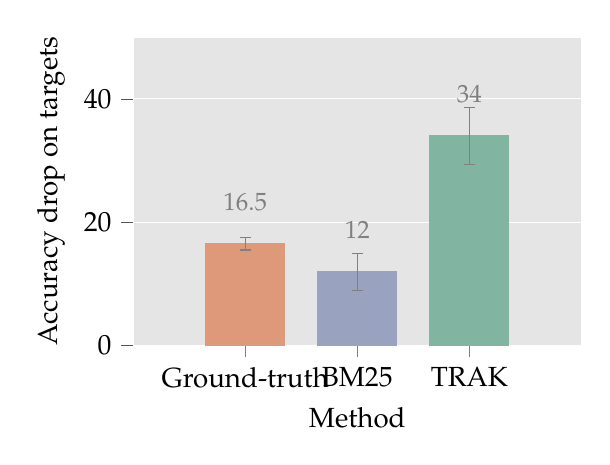
\begin{tikzpicture}
    \definecolor{darkgray141160203}{RGB}{141,160,203}
    \definecolor{dimgray85}{RGB}{85,85,85}
    \definecolor{gainsboro229}{RGB}{229,229,229}
    \definecolor{lightgray204}{RGB}{204,204,204}
    \definecolor{mediumaquamarine102194165}{RGB}{102,194,165}
    \definecolor{orchid231138195}{RGB}{231,138,195}
    \definecolor{salmon25214198}{RGB}{252,141,98}
    \definecolor{amethyst}{rgb}{0.6, 0.4, 0.8}
    \definecolor{bleudefrance}{rgb}{0.19, 0.55, 0.91}
    \definecolor{blush}{rgb}{0.87, 0.36, 0.51}
    \definecolor{brilliantrose}{rgb}{1.0, 0.33, 0.64}
    \definecolor{trakorange}{rgb}{0.87, 0.6, 0.48}
    \definecolor{trakgreen}{rgb}{0.51, 0.705, 0.635}
    \definecolor{trakblue}{rgb}{0.60, 0.64, 0.753}
    \begin{axis}[
        axis background/.style={fill=gainsboro229},
        axis line style={white},
        width=0.6\textwidth,
        height=5.5cm,
        ybar,
        tick align=outside,
        tick pos=left,
        enlarge x limits=0.5,
        ylabel={Accuracy drop on targets},
        xlabel={Method},
        xtick={1,2,3},
        xticklabels={Ground-truth, BM25, TRAK},
        nodes near coords={
            \pgfmathprintnumber[fixed]{\pgfplotspointmeta}
        },
        nodes near coords style={
            yshift=0.3cm,
            text=gray,
            font=\small
        },
        nodes near coords align={vertical},
        ymin=0,
        ymax=1, %
        error bars/y dir=both,
        error bars/y explicit,
        error bars/error bar style={gray},
        bar width={1cm},
        y grid style={white},
        ymajorgrids,
        ymin=0, ymax=50,
        ytick style={color=dimgray85}
        ]
        \addplot[fill=trakorange,
                  draw=trakorange, 
                  bar shift=0cm,
                  error bars/.cd, 
                  y dir=both, 
                  y explicit]
            coordinates{
                (1, 16.5) +- (0, 1)%
            }; 
        
        \addplot[fill=trakblue, 
                  draw=trakblue,
                  error bars/.cd, 
                  y dir=both, 
                  y explicit]
            coordinates {
                (2, 12) +- (3.0, 3.0)
            }; 

        \addplot[fill=trakgreen, 
                  draw=trakgreen,
                  bar shift=0cm,
                  error bars/.cd, 
                  y dir=both, 
                  y explicit]
            coordinates {
                (3, 34) +- (4.8, 4.6)
            }; 
    \end{axis}
\end{tikzpicture}
\caption{{\em Identifying counterfactually important examples for learning facts on \ftracetrex.}
        Given a set of queries that the language model (\texttt{mt5-small}) originally answers correctly after training, we compare how three different interventions---removing abstracts with the highest \trak scores, removing the most similar abstracts according to BM25, and removing the ground-truth proponents as indicated by \ftracetrex---affect the resulting model's accuracy on the queries.
        The $y$-axis shows the {\em decrease} in accuracy (on the query set, relative to the original model) after each intervention; results are averaged over 50 queries and eight independent models.
        Error bars represent $95\%$ confidence intervals.
    }
    \label{fig:nlp_counterfactual}
\end{figure}

\paragraph{Discussion.}
Our results demonstrate that while \trak may not be effective at identifying abstracts
that directly express the same fact as a given query
(i.e., the ground-truth proponents as defined by \ftracetrex),
it {\em can} successfully identify the abstracts that are most
responsible for the finetuned model {\em learning} a given fact.
In particular, \trak's subpar performance on the attribution benchmark
is an artifact of the \ftracetrex benchmark rather than a flaw of \trak itself.

There are several potential explanations for this phenomenon, many of which
\citet{akyurek2022towards} already discuss in their work:
\begin{itemize}
    \item There may be errors in the \ftracetrex benchmark. (Although,
    given the drastic difference between the \trak scores
    and the ground-truth labels in their ability to identify counterfactually important abstracts,
    such data errors are unlikely to be the sole culprit.)
    \item Models may be answering queries by
    {\em combining} facts from the training set.
    For example, neither ``The largest pyramid is in Giza'' nor ``Giza is a city in Egypt'' would be
    ground-truth proponents for the query ``Which country is home to the largest pyramid?'' in \ftracetrex,
    but a model that learns both of these facts
    may still be able to correctly answer that query.
    \item Alternatively, models may be learning from the syntactic rather than
    semantic structure of abstracts. For example, a model may correctly answer
    that a person from Korea is called a ``Korean'' by learning from an
    abstract which says ``A person from Bulgaria is Bulgarian.''
\end{itemize}

More broadly,
our results highlight a difference between {\em fact tracing}
and {\em behavior tracing}.
In other words,
finding a data source that supports a given model-generated text is a different task
than identifying the actual data sources that {\em caused} the model to generate this text in
the first place.
While we may be able to address the former problem with { model-independent}
techniques such as information retrieval or web search,
the latter requires methods that remain faithful to (and thus, dependent on)
the model being studied. Our results here indicate that \trak can be an effective tool for the latter problem.










\subsection{Accelerating datamodel applications}
\label{subsec:datamodel_apps}
Our evaluation thus far has demonstrated that data attribution scores computed with
\trak  can {\em predict} how a given model's output changes as a function of the composition of the corresponding model's training set.
While the capability to make such predictions is useful in its own right, prior
work has shown that this primitive also enables many downstream applications
\cite{koh2017understanding,jia2019towards,alaa2020discriminative}.  For example,
prior works leverage datamodel scores to identify brittle predictions
\cite{ilyas2022datamodels} and to compare different learning algorithms
\cite{shah2022modeldiff}. We now show that using \trak in place of datamodel
scores can significantly speed up these downstream applications too.

\subsubsection{Estimating prediction brittleness}
\citet{ilyas2022datamodels} use datamodel scores to
provide {\em lower bounds} on the {\em brittleness} of a given example---that
is, given an example of interest $z$, they identify a subset of the training set
whose removal from the training data causes the resulting re-trained model to
misclassify $z$.
The brittleness estimation algorithm that \citet{ilyas2022datamodels} leverage
hinges on the fact that the datamodel attribution function $\tau_\text{DM}(z)$
can accurately predict model outputs, i.e., achieve high LDS. Motivated by
\trak's good performance on the linear datamodeling task (see, e.g.,
\cref{fig:headline_full}), we examine estimating the brittleness of \cifarten examples
using \trak scores in place of datamodel ones (but otherwise following the
procedure of \citet{ilyas2022datamodels}). Our results (see
\Cref{fig:brittle}) indicate that \trak scores computed from an ensemble of just
100 models are about as effective at estimating brittleness as datamodel scores
computed from 50,000 models. Thus, \trak scores can be a viable (and orders of
magnitude faster) alternative to datamodels for estimating
prediction brittleness.

\begin{figure*}[t]
    \centering
    \begin{tikzpicture}
    \centering
    \definecolor{darkgray141160203}{RGB}{141,160,203}
    \definecolor{dimgray85}{RGB}{85,85,85}
    \definecolor{gainsboro229}{RGB}{229,229,229}
    \definecolor{lightgray204}{RGB}{204,204,204}
    \definecolor{mediumaquamarine102194165}{RGB}{102,194,165}
    \definecolor{orchid231138195}{RGB}{231,138,195}
    \definecolor{salmon25214198}{RGB}{252,141,98}
    \definecolor{amethyst}{rgb}{0.6, 0.4, 0.8}
    \definecolor{bleudefrance}{rgb}{0.19, 0.55, 0.91}
    \definecolor{blush}{rgb}{0.87, 0.36, 0.51}
    \definecolor{brilliantrose}{rgb}{1.0, 0.33, 0.64}
    \begin{groupplot}[
        group style={group size= 1 by 1, horizontal sep=0cm, vertical sep=0cm},
        height={6cm},
        width=.55\linewidth]
    \nextgroupplot[
        xlabel={\# training examples removed to flip prediction},
        ylabel={Frac. of CIFAR-10 test set},
        legend pos={north east},
        axis background/.style={fill=gainsboro229},
        axis line style={white},
        legend cell align={left},
        legend columns=1,
        legend style={
        fill opacity=0.8,
        draw opacity=1,
        text opacity=1,
        at={(1.05,0.9)},
        anchor=north west,
        draw=gainsboro229,
        fill=gainsboro229,
        },
        ymajorgrids=true,
        no marks,
        xmin=0, xmax=1000,
        xmajorgrids, xminorgrids,
        x grid style={white},
        y grid style={white},
        tick align=outside,
        tick pos=left,
    ]

    \addplot[ultra thick, color=mediumaquamarine102194165] table [x=x, y=y, col sep=comma] {data/brittleness_methods/Datamodel300k.csv};
    \addlegendentry{Datamodels ($300$k models)}

    \addplot[ultra thick, color=black, dashed] table [x=x, y=y, col sep=comma] {data/brittleness_methods/TRAK.csv};
    \addlegendentry{TRAK (100 models)}

    \addplot[ultra thick, color=mediumaquamarine102194165] table [x=x, y=y, col sep=comma] {data/brittleness_methods/Datamodel50k.csv};
    \addlegendentry{Datamodels ($50$k models)}

    \addplot[ultra thick, color=orchid231138195] table [x=x, y=y, col sep=comma] {data/brittleness_methods/TracIn.csv};
    \addlegendentry{TracIn ($100$ models)}

    \addplot[ultra thick, color=blush] table [x=x, y=y, col sep=comma] {data/brittleness_methods/RepresentationSimilarity.csv};
    \addlegendentry{Representation Sim. ($100$ models)}

    \addplot[ultra thick, color=bleudefrance] table [x=x, y=y, col sep=comma] {data/brittleness_methods/InfluenceFunction.csv};
    \addlegendentry{Influence Function ($100$ models)}
    
    \end{groupplot}
\end{tikzpicture}
    \caption{{\em Using \trak scores to identify brittle model predictions.}
    Following the methodology of \citet{ilyas2022datamodels}, we apply
    different data attribution methods to estimate the brittleness of model predictions on
    examples from the \cifarten validation set. The number of models used by each attribution method is specified in parentheses, e.g., \trak
    (100) indicates that \trak scores were computed using an ensemble of 100 trained
    models.}
\label{fig:brittle}
\end{figure*}

\subsubsection{Learning algorithm comparisons}
A useful way to leverage datamodels is to view them as {\em data representations}.
More specifically, following \citet{ilyas2022datamodels}, for an example of interest $z$, one can view the datamodel
attribution $\tau_\text{DM}(z)$ as an embedding of $z$ into $\mathbb{R}^{n}$,
where $n$ is the size of the training dataset.  Analyzing examples in such
induced {\em datamodel representation spaces} turns out to enable uncovering
dataset biases and model-specific subpopulations
\cite{ilyas2022datamodels}.
Furthermore, this representation space is not specific to a particular model
instance or architecture---it is {\em globally aligned} in the sense that for
the same example $z$, the attribution score $\tau_\text{DM}(z)_i$ of a given
train example $i$ has a consistent interpretation across {\em different}
learning pipelines.
\citet{shah2022modeldiff} leverage the properties of the datamodel
representation space to perform model-agnostic {\em learning algorithm comparison}
(called \modeldiff): given two learning algorithms, they show how to
use datamodels to identify {\em distinguishing features}, i.e., features that
are used by one learning algorithm but not the other.



Once again, motivated by \trak's good performance on the LDS metric,
we investigate whether \trak scores can substitute for datamodel scores in this
context. To this end, we revisit one of the case studies from
\citet{shah2022modeldiff}---the one that compares image classifiers trained {with}
and {without} data augmentation, and identifies features that distinguish these
two classes of models.
When applied to this case study, \modeldiff computed with \trak scores recovers similar distinguishing features
to the ones originally found by \citet{shah2022modeldiff} (using datamodel scores)---see \Cref{fig:modeldiff} for more details.
Also, employing \trak scores in place of datamodel scores reduces the total
computational cost by a factor of 100, showing, once again, that \trak can dramatically
accelerate downstream tasks that rely on accurate attribution scores.







\section{Related work}
\label{sec:related}
\section{Related work}
\noindent \textbf{Video foundation models.}
With sufficient computational power and an abundant source of data, there have been attempts to build a single large-scale foundation model that can be adapted to diverse downstream tasks.
Along with the success of foundations models in the natural language processing domain~\cite{brown2020language,chen2021evaluating,devlin2019bert} and in computer vision~\cite{bertasius2021space,jia2021scaling,radford2021learning}, video data has become another data type of interest, as it has grown in scale due to numerous internet video-sharing platforms.
Accordingly, several methods to train a video foundation model have been proposed.
Due to the innate multi-modality of video data, \textit{i.e.}, a combination of visual $\cdot$ vocal $\cdot$ textual context, most works have centered around the variations of the cross-modal attention mechanism \cite{akbari2021vatt,bertasius2021space,gabeur2020multi,luo2020univl,neimark2021video,tan2021look,wei2020multi,yang2021taco}.
In addition, as most video data lack proper labels or descriptions, contrastive learning methods were studied to learn meaningful feature representations or enhance video-text alignment in a self-supervised manner \cite{akbari2021vatt,kuang2021video,luo2020univl,yang2021taco}.

More specifically, MERLOT \cite{zellers2021merlot} proposed a multi-modal representation learning method for visual commonsense reasoning, which also performed well in twelve video reasoning tasks.
VATT \cite{akbari2021vatt} introduced a multi-modal learning method via contrastive learning. 
The pre-trained model performed well in a variety of vision tasks from image classification to video action recognition and zero-shot video retrieval.
Another representative work, UniVL \cite{luo2020univl} proposed a straightforward pre-training method with auxiliary loss functions. 
After fine-tuning on a specific task, the pre-trained model performed outstandingly in a wide range of tasks of text-to-video retrieval, action segmentation, action step localization, video sentiment analysis, and video captioning.
Other foundation models for multiple video tasks include \cite{li2020hero,sun2019learning,sun2019videobert,zhu2020actbert,fu2021violet,wang2022all}. 

\noindent \textbf{Auxiliary learning.}
In order to enhance the performance of one or a multitude of primary tasks, auxiliary learning methods can be incorporated.
\cite{ruder2017overview} introduced Multi-task learning (MTL) to the deep neural networks by training a single model with multiple task losses to assist learning on the main task.
Such a method is generally adapted to pre-train the foundation models in the self-supervised manner~\cite{li2020hero,sun2019learning,sun2019videobert,zhu2020actbert,fu2021violet,wang2022all}.
However, these various pretext task losses used in the pre-training phase are ignored in the fine-tuning phase, and only the primary task loss is minimized.

Recently, meta-learning methods have been introduced for auxiliary learning.
\cite{liu2019self,navon2020auxiliary,shu2019meta} proposed a meta-learning method in which the model learns auxiliary tasks to generalize well to unseen data. 
In these settings, a separate subset of data is held out as the primary task, while the others are used as auxiliary tasks that aid the primary task's performance.
Similar methods were adopted for computer vision tasks such as semantic segmentation \cite{xu2021leveraging}.
Other domain applications include navigation tasks with reinforcement learning \cite{ye2021auxiliary}, or self-supervised learning methods on graph data \cite{hwang2020self}.

\section{Discussion \& Conclusion}
We provide some comments on the growth conditions which constituted the majority of our analysis in sections \ref{sec:Hmixing} and \ref{sec:Hsigma}. In the simplest cases of Lemma \ref{lemma:unstableGrowth}, growth was established in an analogous fashion to the old one-step expansion condition (\ref{eq:oldOneStepExpansion}), finding the relevant Jacobians $M_j$ and checking that their expansion factors $K(M_j)$ satisfy
\begin{equation}
    \label{eq:discussionOneStep}
    \sum_j \frac{1}{K(M_j)} <1.
\end{equation}
For the more complicated cases, the inductive method used to establish growth near the accumulation points in Lemma \ref{lemma:unstableGrowth} and the weakened one-step expansion condition (\ref{eq:oneStep}) both address the same fundamental issue: the splitting of unstable curves by singularities into an unbounded number of small components. They circumvent this obstacle in rather different ways, however. While (\ref{eq:oneStep}) generalises (\ref{eq:discussionOneStep}) to ensure an growth of unstable curves `on average' (see \cite{chernov_statistical_2009} for a precise statement), our inductive method is a more direct adaptation of (\ref{eq:discussionOneStep}), using it to generate contradictory geometric conditions which a hypothetical non-growing unstable curve must satisfy. It may be possible to prove Theorem \ref{sec:Hmixing} using (\ref{eq:oneStep}) as the basis for growth. Since we required (\ref{eq:oneStep}) anyway for proving Theorem \ref{thm:HsigmaExp}, this could potentially condense our analysis, but only to a minor extent. A convenience of the method used in section \ref{sec:Hmixing} is that, by way of the `simple intersection' property, it naturally gives geometric information on the images of manifolds, useful for proving the property \textbf{(M)} of Theorem \ref{thm:katok-strelcyn}.

We expect that essentially analogous analysis can be applied to establish mixing properties in a wide class of piecewise linear non-uniformly hyperbolic maps, including those (like the OTM) which sit on the boundary of ergodicity and beyond. While we have relied on the precise partition structure of $H_\sigma$, its fundamental feature (self-similar sequences of elements $A^k$, sharing boundaries with its neighbours $A^{k-1},A^{k+1}$ and accumulating onto some point $p$) is quite typical to return map systems. See, for example, those of various stadium billiards \cite{chernov_chaotic_2006,chernov_improved_2008,chernov_statistical_2009} and LTMs \cite{springham_polynomial_2014}. Indeed, the same method can be used to prove the Bernoulli property for non-monotonic LTMs \cite{myers_hill_mixing_2022}, where monotonicity of the manifold images cannot be assumed and the classical argument \cite{sturman_mathematical_2006} fails. The OTM is the pointwise limit of these maps as the boundary shrinks to null measure. It further has utility in proving growth conditions for maps which are uniformly hyperbolic but possess regions $A_j$ where the hyperbolicity is very weak, signified by $K(M_j) \approx 1$, so that (\ref{eq:discussionOneStep}) fails. Typically this leads to suboptimal bounds on mixing windows, see e.g. \cite{wojtkowski_model_1981,przytycki_ergodicity_1983,myers_hill_family_2022}. The map $H_{(\eta,\eta)}$ for $\eta \approx 1/2$ is another example, possessing weak hyperbolicity over $A_2, A_3$. Letting $\varepsilon = |\eta-1/2|>0$, there is an upper bound $N = N(\varepsilon)$ on escape times from the intersections $A_2\cap \sigma, A_3 \cap \sigma$. The growth lemma then follows by applying the inductive step roughly $N$ times and can be established for arbitrarily small $\varepsilon$, opening the door to establishing optimal mixing windows.

The above gives two examples of piecewise linear perturbations to $H$ where mixing with respect to Lebesgue is preserved and our methods can be applied. Nonlinear perturbations to the shear profiles complicate the analysis in several ways. Firstly as the map's Jacobians takes on a broader range of values, cone invariance becomes an increasingly harder condition to establish. Cones must be widened, giving looser bounds on expansion factors, which may already be weak due to new regions of weaker stretching. This, together with the change from polygonal to curvilinear return time partition elements and nonlinear local manifolds, adds some complexity to showing growth conditions. This does not rule out certain (small) nonlinear perturbations however. There is some leeway in the inequalities which govern cone invariance and growth of local manifolds, the latter of which is not too dissimilar from the piecewise linear setting (see Lemmas \ref{lemma:piecewiseApprox}, \ref{lemma:componentLength}). Certain small perturbations would not alter the \emph{topological} structure of the return time partition, i.e. which elements share boundaries, the key information needed for setting up the induction. Finally while the partition elements would no longer be polygonal, only coarse geometric information is required for verifying each inductive step. Following the above, a potential perturbation could be to replace the linear portions of each shear by a cubic, perturbing the tent profile
\[  f(t) = \begin{cases} 2t & 0 \leq t \leq 1/2, \\ 2(1-t) & 1/2 \leq t \leq 1 ,\end{cases} \]
of the OTM shears to
\[  f_a(t) = \begin{cases} \frac{1}{8} t \left(16 - a + 6at - 8at^{2} \right) & 0 \leq t \leq 1/2, \\ \frac{1}{8}\left(1-t\right)\left( 16 - a + 6a\left(1-t\right) - 8a\left(1-t\right)^{2}\right)  & 1/2 \leq t \leq 1, \end{cases}   \]
for $a>0$. For small enough $a$ the gradient range $f'(t)$ is restricted to small neighbourhoods of $\{ 2, -2\}$ and the escape time partition retains a similar structure. We illustrate this in Figure \ref{fig:perturbations}, showing escapes from the square $S_3$ under the map $G \circ F$, equivalent to escapes from the perturbed $A_3$ under the $G \circ F$, but with a cleaner geometry for comparison. When $a$ is too large the analogy to the OTM breaks down. At $a=16$ the map is twice differentiable everywhere and features a new source of slowed mixing, the Jacobian is the identity at the corner points $x,y \in \{  0, 1/2 \}$ giving locally parabolic behaviour (visible in the escape time partition). 

\begin{figure}
    \centering
    \includegraphics[width=0.24 \linewidth]{0.png}
    \includegraphics[width=0.24 \linewidth]{4.png}
    \includegraphics[width=0.24 \linewidth]{8.png}
    \includegraphics[width=0.24 \linewidth]{16.png}
    \caption{Partition of escape times from $S_3$ under the mapping $F \circ G$ for $a= 0,4,8,16$. }
    \label{fig:perturbations}
\end{figure}


\clearpage
\section*{Acknowledgements}
We thank Ekin Akyurek for help 
installing and using the \ftracetrex benchmark.

Work supported in part by the NSF grants CNS-1815221 and DMS-2134108, and Open Philanthropy. This material is based upon work supported by the Defense Advanced Research Projects Agency (DARPA) under Contract No. HR001120C0015.

Research was sponsored by the United States Air Force Research Laboratory and the United States Air Force Artificial Intelligence Accelerator and was accomplished under Cooperative Agreement Number FA8750-19-2-1000. The views and conclusions contained in this document are those of the authors and should not be interpreted as representing the official policies, either expressed or implied, of the United States Air Force or the U.S. Government. The U.S. Government is authorized to reproduce and distribute reprints for Government purposes notwithstanding any copyright notation herein.

\printbibliography

\clearpage
\appendix
\addcontentsline{toc}{section}{Appendix} %
\renewcommand\ptctitle{Appendices}
\part{}
\parttoc
\clearpage

\counterwithin{figure}{section}
\counterwithin{table}{section}
\counterwithin{algorithm}{section}


\section{Experimental Setup}
\label{app:exp_setup}
%% Macro setup
\definecolor{purple}{rgb}{1, 0, 1}

\newcommand{\ie}{\emph{i.e.,}\xspace}
\newcommand{\eg}{\emph{e.g.,}\xspace}
\newcommand{\abr}{\emph{abbr.}\xspace}
\newcommand{\ea}{\emph{et al.}\xspace}
\newcommand{\gensync}{\emph{GenSync}\xspace}
\newcommand{\colosseum}{\emph{Colosseum}\xspace}
\newcommand{\srep}{\emph{SREP}\xspace} % Set Reconciliation Enhances
\newcommand{\srepsim}{\emph{SREPSim}\xspace}
% Propagation
\newcommand{\esrep}{\emph{E-SREP}\xspace}
\newcommand{\epsrep}{\emph{EP-SREP}\xspace}
\newcommand{\mesrep}{\emph{ME-SREP}\xspace}
\newcommand{\mempoolsync}{\emph{MempoolSync}}

\newcommand{\fref}[1]{Fig.~\ref{#1}}
\newcommand{\tref}[1]{Table~\ref{#1}}
\newcommand{\aref}[1]{Algorithm~\ref{#1}}
\newcommand{\procref}[1]{Procedure~\ref{#1}}
\newcommand{\sref}[1]{Section~\ref{#1}}
\newcommand{\lineref}[1]{line~\ref{#1}}
\newcommand{\appref}[1]{Appendix~\ref{#1}}

% Change \eqref
\LetLtxMacro{\originaleqref}{\eqref}
\renewcommand{\eqref}{Eq.~\originaleqref}

% Theorems and corollaries
\newcounter{theoremcount}
\setcounter{theoremcount}{0}
\DeclareRobustCommand{\theorem}[1]{%
  \refstepcounter{theoremcount}%
  \noindent\textit{\textbf{Theorem \thetheoremcount\label{theorem:#1}: }}%
}
\DeclareRobustCommand{\theoremref}[1]{Theorem~\ref{theorem:#1}}

\DeclareRobustCommand{\proof}{\emph{Proof:}\xspace}
\DeclareRobustCommand{\qqed}{\hfill$\blacksquare$}

\newcounter{corollcount}
\setcounter{corollcount}{0}
\DeclareRobustCommand{\coroll}[1]{%
  \refstepcounter{corollcount}%
  \noindent\textit{\textbf{Corollary \thecorollcount\label{coroll:#1}: }}%
}
\DeclareRobustCommand{\corollref}[1]{Corollary~\ref{coroll:#1}}

\newcounter{lemmacount}
\setcounter{lemmacount}{0}
\DeclareRobustCommand{\lemma}[1]{%
  \refstepcounter{lemmacount}%
  \noindent\textit{\textbf{Lemma \thelemmacount\label{lemma:#1}: }}%
}
\DeclareRobustCommand{\lemmaref}[1]{Lemma~\ref{lemma:#1}}

\newcounter{definitioncount}
\setcounter{definitioncount}{0}
\DeclareRobustCommand{\definition}[1]{%
  \refstepcounter{definitioncount}%
  \noindent\textit{\textbf{Definition \thedefinitioncount\label{definition:#1}: }}%
}
\DeclareRobustCommand{\defref}[1]{Definition~\ref{definition:#1}}

%notes of different authors
\newif\ifnotes
\notestrue
\notesfalse

\newif\ifdiff
\difftrue
\difffalse

\newcommand{\anote}[1]{\ifnotes $\ll$\textsf{\textcolor{purple}{Ari: {#1}}}$\gg$ \fi}
\newcommand{\nnote}[1]{\ifnotes $\ll$\textsf{\textcolor{orange}{Novak: {#1}}}$\gg$ \fi}
\newcommand{\diff}[1]{\ifdiff\textcolor{orange}{#1}\else#1\fi}

%%% Local Variables:
%%% mode: latex
%%% TeX-master: "main"
%%% End:


%%% Redefining theorem-like environments
\newcounter{environments}

\newcounter{theoremCounter}
\newcounter{lemmaCounter}
\newcounter{definitionCounter}
\newcounter{propositionCounter}
\newcounter{corollaryCounter}
\newcounter{exampleCounter}
\newcounter{remarkCounter}
\newcounter{propertyCounter}
\newcounter{assumptionCounter}
\newcounter{proofCounter}

%\theorempreskip{1pt}
%\theorempostskip{1pt}

\let\proposition\relax
\let\theorem\relax
\let\lemma\relax
\let\definition\relax
\let\corollary\relax
\theoremseparator{.}
\theorembodyfont{\itshape}
\theoremsymbol{$\triangleleft$}
\newtheorem{theorem}[theoremCounter]{Theorem}
\newtheorem{lemma}[lemmaCounter]{Lemma}
\newtheorem{definition}[definitionCounter]{Definition}
\newtheorem{proposition}[propositionCounter]{Proposition}
\newtheorem{corollary}[corollaryCounter]{Corollary}

\let\remark\relax
\let\example\relax
\let\assumption\relax

\theorembodyfont{\normalfont}
\newtheorem{example}[exampleCounter]{Example}
\newtheorem{remark}[remarkCounter]{Remark}

\theoremheaderfont{\itshape}
\theoremsymbol{}
\renewtheorem{property}[remarkCounter]{Property}

\theoremheaderfont{\bfseries}
\theorembodyfont{\itshape}
\newtheorem{assumption}[assumptionCounter]{Assumption}
\theoremheaderfont{\itshape}


\theoremstyle{plain}
\theoremheaderfont{\itshape}
\theorembodyfont{\normalfont}
\let\proof\relax
\theoremseparator{.}
\theoremsymbol{\qedfull}
\newtheorem*{proof}{Proof}
\qedsymbol{\qedfull}

% Reset equation counters for each property!
\makeatletter
\@addtoreset{equation}{property}
\makeatother

% Tikz stuff
\newcommand{\seqarr}
{\begin{tikzpicture}
		\draw[-{Triangle[scale=.7]}] (0,0) --  (.3,0); 
\end{tikzpicture}}

\newcommand{\looparr}
{\begin{tikzpicture}[scale=0.7,baseline=-1.55ex]
		\draw[arrows = {-Stealth[inset=0pt, length=2pt, angle'=60]}] (0,0) arc (102:437:.2cm);
\end{tikzpicture}}

\definecolor{blue-violet}{rgb}{0.54, 0.17, 0.89}
\definecolor{cadmiumorange}{rgb}{0.93, 0.53, 0.18}
\definecolor{yellow-green}{rgb}{0.6, 0.8, 0.2}
\definecolor{green1}{rgb}{0.12, 0.3, 0.17}
\definecolor{byzantium}{rgb}{0.44, 0.16, 0.39}


\clearpage
\section{\trak implementation}
\label{app:impl}
\section{Implementation}
\label{sec:impl}

At \company, we have deployed \sysname in our internal clusters to serve daily DL workloads.
The internal clusters consist of heterogeneous GPUs, including NVIDIA T4 GPU and NVIDIA A10 GPU.
Integrated with Kubernetes~\cite{k8s}, \sysname manages thousands of GPUs in each cluster and more than 20,000 GPUs in all.

\parabf{Service manager.}
For online workloads, we use the existing service manager at \company which deploys containers, discovers service, and autoscales horizontal pods.

\parabf{Global manager.}
We modify the Kubernetes scheduler to schedule offline workloads.
The workload profiler takes several dedicated GPUs, whose number is negligible to the total number of GPUs.
When a new offline workload comes, the workload profiler performs a few dry runs of the workload and utilizes the NVIDIA Data Center GPU Manager (DCGM) tools~\cite{dcgm} and NVIDIA Management Library (NVML)~\cite{nvml} libraries to collect GPU metrics.
We collect about 2,000 data for each GPU type to train the speed predictor.
The MLPs of the speed predictor have four layers with hidden size $64\times 64$.
The MLPs are trained with momentum SGD optimizer~\cite{ruder2016overview} in PyTorch v1.8.0~\cite{paszke2019pytorch} until they converge.
\sysname invokes the scheduler periodically to schedule all offline workloads.
When moving workloads, we record checkpoints of offline workloads and restart the workloads after transmitting the models and checkpoints.
As the datasets are usually colossal, we store the datasets in a remote file system and fetch data during the execution.
We implement the scheduler as a third-party plugin to the Kubernetes scheduler.


\parabf{Local executor.}
Each local executor executes online workloads according to the service manager and offline workloads according to the global manager.
DL workloads are executed in Docker containers with our customized components.
We add Best-Effort GPU DevicePlugin in Kubernetes and relevant control paths with Kubelet and \sysprobe for offline workloads.
To control SM percentage, we leverage the environment variable $CUDA\_MPS\_ACTIVE\_THREAD\_PERCENTAGE$ provided by MPS.
The GPU monitor collects resource metrics through DCGM~\cite{dcgm} and NVML~\cite{nvml} for NVIDIA GPU.
The \sysprobe updates the state machine with the collected resource metrics and empirically-set thresholds.
When the state is unhealthy, the \sysprobe will ask the NodeManager in Kubernetes to evict offline workloads.
\bytecuda intercepts nearly 800 CUDA driver APIs for GPU memory allocation and kernel launch.
The GPU memory quota of offline workloads is fixed to $40\%$ as Figure~\ref{fig:motiv_gpu_resource} reports that most online workloads use less than $60\%$ GPU memory.
We adopt the cpuset of Cgroup for CPU isolation.
For memory, \sysname will evict offline workloads if memory usage is higher than a threshold or the kernel swap daemon is busy for a long time.
The parameters to calculate GPU load in Equation~\ref{equ:gpu_load}$\&$\ref{equ:clock_factor} are empirically selected through trial-and-error.


\clearpage
\section{Theoretical Justification}
\label{app:theory_extra}
\section{Design}
\label{s:design}
In this section, we will first present the core of our system. Then we present some analysis of the system along with some extensions to address a few practical concerns. We will present details of our cloud implementation separately in the next section.

\subsection{Delivery Based Ordering}
Our solution is composed of three parts. 
\subsubsection{Delivery Clock\\}
\noindent\textbf{What we do.}
Each RB maintains a delivery clock. This delivery clock essentially tracks time relative to when market data was delivered to the participant. We use $DC(i,a)$ to represent delivery clock of participant $i$ at time when trade $(i,a)$ is submitted. Delivery clock is a lexicographical tuple.
\begin{align}
    DC(i,a) = \langle ld(i,a), S(i,a)-D(i, ld(i,a))\rangle.
\end{align}
where $ld(i,a)$ is the latest data point that was delivered to MP$_i$ by time S(i,a), i.e., $D(i,ld(i,a)) \leq S(i,a) < D(i,ld(i,a)+1)$). 
Interval, $S(i,a)-D(i, ld(i,a))$, corresponds to the time that has elapsed since the last delivery and can be measured locally at the RB without requiring any clock synchronization (challenge 1). 

\noindent
\textit{Monotonicity:} Delivery clocks advance monotonically with submission time. As a result, DBO trivially satisfies the causality condition (Equation~\ref{eq:causality}). Further, it incentivizes the participants to submit trades as early as possible. Therefore, \emph{a participant cannot gain any advantage by delaying trades.} %\pg{should this point have a heading of its own}
Finally, we also leverage the monotonic property to overcome challenge 3 (\S\ref{ss:enforcing_ordering}). Figure~\ref{fig:delivery_clock} shows how delivery clock advances with time.

%\pg{I tried to reduce the notation here. I defined delivery clock slightly differently.}

\begin{figure}[t]
\centering
    \includegraphics[width=0.8\columnwidth]{figures/delivery_clock.pdf}
    \caption{\small{\bf Delivery Clock.}}% \pg{Redraw}}% \pg{Eashan see Ranveer's comment}}% \pg{Eashan can you redraw this figure in powerpoint or something.}}}
    \label{fig:delivery_clock}
    \vspace{-2.5mm}
\end{figure}

All incoming trades are marked with the delivery clock at the trade submission time. The ordering buffer uses this delivery clock time to order trades. Formally, the ordering in DBO is given by,  

\vspace{-2mm}
\begin{align}
    O(i,a) = DC(i, a). 
    \label{eq:ordering_with_dc}
\end{align}


\begin{figure}[t]
\centering
    \includegraphics[trim={0 0 0 2mm},clip,width=0.8\columnwidth]{figures/dbo_correct.pdf}
    \vspace{-4mm}
    \caption{\small{{\bf DBO can help correct for late delivery of data.} Delivery of market data to MP$_i$ is lagging behind MP$_j$. There are two trades $(i,a)$ and $(j,b)$ generated in response to the same market data $x$. $(j,b)$ was submitted before $(i,a)$ but
    %, i.e., $S_j(l) < A_i(k)$. 
    response time of $(i,a)$ is less than $(j,b)$.
    %, i.e., $rt_i(k) < rt_j(l)$. 
    In this example, $DC(i,a) (= \langle x, RT(i,a)\rangle) < DC(j,b) (= \langle x, RT(j,b)\rangle)$ and trade $(i,a)$ is correctly ordered ahead of $(j,b)$.}} %Ordering based on the submission time leads to incorrect ordering.}
    %\pg{Correct figure}}
    \label{fig:dbo_correction}
    \vspace{-3mm}
\end{figure}


\noindent\textbf{Why it works.}
When the trigger point of trade $(i,a)$ is indeed the last data point (i.e., $x = TP(i,a) = ld(i, a)$), then, DBO respects condition C2 for LRTF. Figure~\ref{fig:dbo_correction} shows an illustrative example of this.
This is because, the delivery clock directly tracks the response time of $i,a$ in this case and $O(i,a) = DC(i, a) = \langle x, RT(i,a)\rangle$. For a competing trade $(j,b)$ with higher response time, the delivery clock at time of submission will either read $O(j,b) = DC(j, b) = \langle x, RT(j,b)\rangle$ (if S(j,b)<D(j,x+1)) or $DC(j, b) = \langle y, S(j,b)-D(j,y)\rangle$ with $y>x$. In both cases, $O(i,a) < O(j,b)$.


At a high level, in our ordering we are correcting for latency differences in data delivery by using the delivery time of the last data point. When the last data point is not the trigger point for trade $(i,a)$, DBO satisfies the LRTF condition C2, if the following condition holds, 
\begin{align}
    D(i,ld(i,a))-D(i,x) = D(j,ld(i,a))-D(j,x),
    \label{eq:cond_delivery_lrtf}
\end{align}
where $x = TP(i,a)$.  
While it is impossible to ensure that inter-delivery times remain the same for all participants for all points, by pacing data at the RB it is indeed possible to ensure that the above condition is always met.% \radhika{you meant C2 or the above condition?}. \pg{the above condition only}
The main reason why we can meet the above condition is that condition C2 limits that the trigger point $x$ cannot be any arbitrary data point in the past, and that the trigger point must have been delivered recently  $S(i,a)-D(i,x) < \delta$.
%and we only need to ensure same inter-delivery times for. 
In the next subsection, we will show how we can achieve this and solve challenge 2. %\pg{Is this easy to follow?}



%\pg{FIX: say delivery clocks helps correct has static differences in latency. Why are delivery clocks so good on their own, give more intuition and experimentation. Potential things to include, see 6.1. Maybe make a section of.delivery clock on its own. correct the equation here in terms of response time as well.}
%\pg{Should we include results on necessary conditions on delivery times for achieving LRTF. Maybe its a bit of an overkill.}

\noindent
\textit{Remark:} In our cloud experiments, we find that DBO achieves fairness with very high probability. This is because network latency (from CES to any given participant) exhibits temporal correlation in latency especially over  short periods of time. When temporal correlation is high, inter-delivery time at any participant is close to the inter-generation time at the CES. In such cases, condition given by Equation~\ref{eq:cond_delivery_lrtf} is satisfied with high probability.

\noindent
\textbf{Difference with traditional logical clocks:} Logical clocks are commonly used in distributed systems. The most famous ones are lamport clocks~\cite{lamportSeminalPaper} and vector clocks. These clocks can be used for achieving total causal ordering of events. While these clocks can track causality of events, they cannot be used to achieve response time fairness. In particular, these clocks don't say anything about how two competing trades generated using the same market data should be ordered as these two trades have no direct causality relation. Unlike delivery clocks, such logical clocks also have no notion of measuring time between occurrences of two events. Time difference between events is critical to achieve fairnesss for exchanges. 

\noindent\textit{Note:} Several major financial exchanges already rely on heartbeats~\cite{nyse-client} for liveness when traffic is low.


\begin{figure}[t]
\centering
    \includegraphics[width=0.8\columnwidth]{figures/batching_pacing.pdf}
    \vspace{-2mm}
    \caption{\small{\bf Batching and Pacing. Inter-delivery time for consecutive batches is equal to or more than $\delta$.}}% \pg{Redraw}}% \pg{Eashan see Ranveer's comment}}% \pg{Eashan can you redraw this figure in powerpoint or something.}}}
    \label{fig:batching_pacing}
    \vspace{-4.5mm}
\end{figure}

\subsubsection{Batching and Pacing\\}
\noindent
\textbf{What we do.}
In DBO, the CES breaks data into batches. Each new batch contains all data points in the duration $(1+\kappa) \cdot \delta$ after the previous batch. Here $\kappa > 0$. Each release buffer delivers all data points in a batch at the same time. %Two points $x,y$ belonging to the same batch are delivered simultaneously to each participant, i.e., $D(j,y)=D(j,x), \forall j$.
The release buffer delivers batches as quickly as possible while ensuring that the time between delivery of two consecutive batches is atleast $\delta$. Figure~\ref{fig:batching_pacing} shows an illustration of batching. Both batching and pacing increase the delivery time of data points. In the next subsection we will analyze the impact of the two on latency. Note that in the event of queue build up at the RB, since the batch generation rate ($\frac{1}{(1+\kappa) \cdot \delta}$) is slower than the batch dequeue rate($\frac{1}{\delta}$), the queue at the RB eventually gets drained(\S\ref{ss:understanding_latency}).


\noindent
\textbf{Why it works.} With batching and pacing, DBO achieves LRTF. In particular, 
consider a trade $(i,a)$ with response time less than $\delta$. Because of pacing, consecutive batches are separated atleast by $\delta$. This means that the trigger point ($x=TP(i,a)$) must be within the last received batch. The point $ld(i,a)$ is also the last point in this batch and $D(i,ld(i,a)) = D(i,x)$. \emph{With batching and pacing, the delivery clock again directly tracks the response time of $(i,a)$} and $O(i,a) = DC(i,a) = <ld(i,a), RT(i,a)>$.
With batching, for participant $j$, $x$ and $ld(i,a)$ also belong to the same batch $D(j,ld(i,a)) = D(j,x)$.
For a competing trade $(j,b)$ with higher response time, the delivery clock at the time of submission will either read $O(j,b) = DC(j,b)) = \langle ld(i,a)), RT(j,b)\rangle$ (if $(j,b)$ was submitted before the next batch, i.e., $S(j,b) < D(j,ld(i,a)+1)$) or $DC(j, b) = \langle y, S(j,b)-D(j,y)\rangle$ with $y>ld(i,a)$. In both cases, $O(i,a) < O(j,b)$.

\if 0
\begin{figure}[t]
\centering
    \includegraphics[width=0.8\columnwidth, angle = -90]{images/pq_hb.jpg}
    \vspace{-2.5mm}
    \caption{\small{\bf Enforcing the ordering.} \pg{Redraw}}% \pg{Eashan see Ranveer's comment}}% \pg{Eashan can you redraw this figure in powerpoint or something.}}}
    \label{fig:pq_hb}
    \vspace{-2.5mm}
\end{figure}
\fi

\subsubsection{Enforcing the ordering\\}
\label{ss:enforcing_ordering}
OB contains a priority queue where all incoming trades are sorted based on the delivery clock timestamp (Equation~\ref{eq:ordering_with_dc}). A trade $(i,a)$ at the head of the priority queue should be forwarded to the CES only when the OB has received all trades $(j,b)$ with lower ordering $DC(j,b) < DC(i,a)$. 

\noindent
\textit{OB's Heartbeat Handler:} In DBO, each RB sends a heartbeat periodically every $\tau$ seconds to the CES. The heartbeat $(i,h)$, from participant $i$ contains the delivery clock timestamp at the time the heartbeat was generated ($DC(i,h)$). Since data in delivered in order and because delivery clock advances monotonically with time, heartbeat $(i,h)$ tells the OB that it has received all trades from participant $i$ with delivery clock less than $DC(i,h)$. The ordering buffer forwards trade $(i,a)$ if it has received heartbeats from all the participants with delivery clock timestamp higher than $DC(i,a)$. 


\subsection{Understanding DBO}

\subsubsection{Latency, parameter setting and straggler mitigation\\}
\label{ss:understanding_latency}

We will first derive the optimal latency for any ordering system that achieves response time fairness. We will then discuss how DBO compares to  optimal latency. We will also present guidelines for setting parameters and how to mitigate stragglers that can impact latency.

We define latency for trade $(i,a)$, $L(i,a)$, as the sum of latency in delivering data (from generation time) and latency in trade forwarding to the CES (from trade submission time). Formally,
\begin{align}
    L(i,a) = (D(i, x) - G(x)) + (F(i,a) - S(i,a)),\nonumber\\
    L(i,a) = F(i,a) - G(x) - RT(i,a),
    \label{eq:latency_def}
\end{align}
where $x=TP(i,a)$.

\noindent
\textbf{Optimal Latency:} Formally trade $(i,a)$ can only be forwarded to the CES's ME only when the CES has received all potential competing trades $(j,b)$ with lower response times ($RT(j,b) < RT(i,a)$). Let $R(i, x, RT)$ represent the time when the CES receives trade $(i,a)$ whose whose trigger point is x and response time is RT. Formally, 
\begin{align}
    F(i,a) = \max_{j}(R(j, x=TP(i,a), RT=RT(i,a))). 
\end{align}
A subtle point to note here is that even if participant $j$ does not produce any trades, we still need to wait for that participant till $R(j, x=TP(i,a), RT(i,a))$. Before this time, fundamentally the CES cannot be sure that it will not receive a trade from participant $j$ with a lower response time. 

We use $RTT(i, x, RT)$ to represent the sum of raw network latency for point x from CES to MP $_i$ and latency of trade from MP$_i$ to the CES (whose trigger point is x and response time RT).  In the best case scenario for latency (no buffering at any point in the path) we get
\begin{align}
    R(i, x, RT) = G(x) + RTT(i, x, RT) + RT.
\end{align}


Using the above two equations, we can write the following theorem.
\begin{theorem}
For any ordering system that achieves response time fairness, the minimum latency for trade $(i,a)$ is given by,
\begin{align}
    L(i,a) = \max_{j}(RTT(j, x=TP(i,a), RT=RT(i,a))).
\end{align}
\vspace{-2mm}
\label{thm:latency}
\end{theorem}

Put it simply, the above theorem states for achieving response time fairness, the minimum latency is bounded by the maximum round trip time across all participants. This means that fundamentally bad latency for a participant affects the latency of all trades. To achieve low latency consistently, we would like to ensure that latency of all the participants is well behaved majority of the times. How to better achieve this goal is left as a subject for future work.

%This theorem implies that even in cloud settings exchanges should ask for  network latency  

%With a very large number of participants thus pose a 
%\pg{fundamental issue with scalability}

\noindent
\textbf{How does DBO compare with the optimal?} DBO achieves close to optimal latency.  Compared to the optimal, batching and pacing introduce additional delay in delivery of market data points.  Since heartbeats are  generated only periodically they can  introduce an additional delay of $\tau$ at the ordering buffer. We now discuss the delay due to each of these components and how do the parameters $\kappa$, $\delta$ and $\tau$ affect latency. %\pg{Include a table here for parameters?}

\noindent
\textbf{Impact of batching:} Batching can introduce an additional delay of $(1+\kappa)\cdot \delta$ in the worst case. 

\noindent
\textit{Setting $\delta$:} $\delta$ thus presents a trade-off between latency and fairness (how large of a horizon can we pick). The right trade-off really depends on the needs of the exchange. Ideally, the exchange should pick the minimum value of $\delta$ that accommodates the response time of the fastest participants in a race. Our conversations reveal that fastest participants typically respond within a few microseconds and majority of the speed races last 5-10 $\mu s$. For our cloud experiments we  use $\delta = 20 \mu s$.

\begin{figure}[t]
    \centering
    \includegraphics[trim={0 0 0 0mm},clip,width=0.8\linewidth]{images/latency_b+p.pdf}
    \vspace{-5mm}
    \caption{\small{\textbf{Latency in data delivery:} x-axis shows the generation time of the market data. y-axis shows the latency from generation time to data delivery. $\kappa$  governs the average slope of the orange line immediately after latency spike (slope = $\frac{\kappa}{1+\kappa}$}).} %\pg{Include orange line and the base latency. Change labels to DBO and direct-delivery. Slope is $\kappa/(1+kappa)$}}
    %\pg{Eashan: Include the drain rate, make the colored lines thicker and use different linestyles for the three schemes..}}% \pg{Maybe label the drain rate in the figure for S1 and S2.}}
    \label{fig:latency_b+p}
    \vspace{-5mm}
\end{figure}

\noindent
\textbf{Impact of pacing.} Pacing restricts the batch dequeue rate at the RB. When network latency to a participant is not varying, the batch arrival/enqueue rate at the RB ($\frac{1}{(1+\kappa) \cdot \delta}$) is higher than the batch dequeue rate limit ($\frac{1}{\delta}$) and there is no queue build up. However, when network latency to a participant is decreasing (e.g., after a latency spike), batch arrival rate at the RB can exceed the dequeue rate limit leading to a queue build up. The overall queue - dequeue rate can be given by $\text{batch size} \cdot \text{batch rate limit} = 1+\kappa$. Figure~\ref{fig:latency_b+p} shows the impact of batching and pacing on latency in delivery of data in the event of a queue build up. The figure also shows the latency when data is delivered directly (raw network latency). The smaller sawtooths in the batching + pacing are because of batching. The deviation in direct delivery and batching + pacing is because of the rate limit imposed by pacing.

\noindent
\textit{Setting $\kappa$:} Increasing $\kappa$ increases batching delay but also increases the queue drain rate in the event of queue build up due to tail latency spikes. Increasing $\kappa$ thus presents a trade-off between reducing tail latency and increasing average latency. In our experiments we use $\kappa = 0.25$.
 
\noindent\textbf{Impact of heartbeats:} Heartbeats present a trade-off. Too frequent heartbeats can overwhelm the network, the ordering buffer or the release buffer. 
Infrequent heartbeats can increase the time OB has to wait of the participants. In particular, hearbeats can introduce an additional wait time of $\tau$. Note that the number of heartbeats, the OB needs to process increases linearly with the number of participants. In the next section we show how the heartbeat handler can be sharded for scalability.

\noindent\textit{Setting $\tau$:} Ideally we want to pick as low of a value as possible for the heartbeats without overwhelming the system. This number is very much dependent on the capabilities of the network and the processing power of the RB and the OB. In our cloud implementation we use $\tau = 20 \mu s$.

\noindent\textit{A note on latency:} When the network latency to participants is not varying with time, there is no queue build up at the release buffers. In such cases, DBO adds maximum of $((1+\kappa)\cdot \delta) + \tau$ additional latency over the optimal.

\noindent\textbf{Straggler Mitigation and RB/MP failure} In the event a  participant or release buffer crashes, DBO can stall processing trades. Further, the overall system latency also gets impacted when a certain participant is experiencing unusually high network latency (see Theorem~\ref{thm:latency}). Here we have the option to wait for the delayed participant and take a latency hit but not let the fairness be impacted. Ideally, we want to let the system continue with low latency with only the affected participant incurring unfairness. In DBO, we use a simple strategy to mitigate this. Using the heartbeats and the generation time of data points, the OB tracks the round trip latency to each participant. If this latency goes beyond a certain threshold for a participant, then the OB does not wait for heartbeats from such straggler participant before forwarding trades. When the round trip latency goes down, OB again starts waiting for heartbeats from the straggler. In the event of crashes, OB might not hear any heartbeats. If the OB does not hear a heartbeat from a particular participant for the above threshold, then it concludes that round trip latency exceeds the threshold and the OB deems the participant a straggler. 
 
\noindent\textit{OB failure:} In the event, the OB crashes all trades in the priority queue will be lost. System will incur unfairness in such cases. 

%The above strategy is also helpful in controlling overall system latency when a certain participant is experiencing unusually high network latency.


\subsubsection{Is Batching and Pacing necessary?\\}
\textbf{Batching and pacing contribute delays; are they necessary?} The answer is yes. Similar to Lemma~\ref{lemma:inter_delivery_imp}, we can derive the necessary conditions for achieving LRTF. 
\begin{corollary}
When trigger points are unknown, the \textit{necessary} conditions on the delivery processes for achieving response time fairness with any ordering system is given by,
\vspace{-1mm}
\begin{align*}
    \text{If }  D(i,y) - D(i,x) &< \delta, \text{ then},\nonumber\\
    D(i, y) - D(i,x) &= D(i,y) - D(i,x), & \forall i,j.
\end{align*}
\label{cor:inter_delivery_lrtf}
\vspace{-6mm}
\end{corollary}

\begin{proof}
Please see Appendix~\ref{app:cor_inter_delivery_lrtf}.
\end{proof}
\vspace{-1mm}
In contrast to Lemma~\ref{lemma:inter_delivery_imp}, the above condition states that the inter-delivery time of two points should be same across all participants only if they are separated by less than $\delta$ for some participant. Batching and pacing indeed satisfies this, for two points x and y in a batch, the inter-delivery times across all participants is indeed zero and hence equal. For point $x$ and $y$ belonging to different batches, since the inter-delivery time is greater than $\delta$ across all participants, there is no additional contraint on inter-delivery times being equal.
 
\subsubsection{Impact of RB to MP latency\\}
In scenarios where RB and the participant cannot be colocated, DBO can incur unfairness. If this latency is unbounded, then, it might be impossible to achieve fairness. If latency is bounded, however, then DBO provides the following fairness guarantees.

\begin{theorem}
    If round trip network latency from release buffer $i$ to it's corresponding participant is bounded between $B_l(i)$ and $B_h(i)$, then, DBO achieves the following guarantee for ordering trades.
    \begin{align*}
    C3: &\text{ if } TP(i,a)= TP(j,b) = x\\ 
    &\land RT(i,a) < RT(j,b) - (B_h(i)-B_l(j)), \\
    & \land RT(i,a) < \delta - B_h(i),\\
    &\text{ then, }O(i,a) < O(j,b).
\end{align*}
    \label{thm:rb_to_mp_latency}
    \vspace{-5mm}
\end{theorem}

\vspace{-1mm}
\begin{proof}
See Appendix~\ref{app:rb_to_mp_latency}.
\end{proof}
\vspace{-1mm}

Compared to LRTF, the above condition reduces the bound on response time for the faster trade $(i,a)$ to $\delta - B_h(i)$.
Additionally, the above condition states that trades are ordered fairly only when the response time of the faster trade is lower than the response time of the competing trade by atleast the variability in latency ($B_h(i)-B_l(j)$). This theorem essentially states that when RB and MP cannot be colocated, for better fairness we should ensure that latency between them is both consistent (across participants) and the upper bound is small.



\subsubsection{Impact of Losses\\}

Although infrequent, packet losses can occur in cloud environments. Such losses can impact fairness in DBO. However, only the fairness for trades that are lost and trades  whose trigger point is lost is impacted (see Appendix~\ref{app:impact_losses}).



\if 0
\subsubsection{Excessive queing at RB and OB\\}
\pg{This can be cut?}

Even though DBO employs straggler mitigation to limit the latency at the OB, it can build up a large queue if it receives a very large number of trades (little's law). The RB can also overflow in scenarios where the network latency is decreasing (Figure~\ref{fig:latency_b+p}) for a large period of time. 

\noindent
\textbf{RB:} In the event a release buffer's queue fills up (exceeds a certain threshold), to avoid overflow the release buffer forgoes pacing and starts releasing data as fast as possible to reduce the queue. In such cases, the delivery clock advances faster than as dictated by pacing. As a result, trades from such a participant might unfairly get ordered behind. The fairness for trades from other participants remains unaffected. When the queue goes down the RB resumes normal operation.

\noindent
\textbf{OB overflow:} In the event the order buffer's queue fills up, the OB starts releasing trades as fast as possible without waiting for heartbeats from participants. Once the queue goes down, OB resumes normal operation. In such cases, fairness of all trades are impacted. 
\fi

\subsubsection{Thwarting front-running attacks\\}

%Monotonicity of delivery clocks ensures that participants are incentivized to submit trades as early as possible and delaying trades does not offer any competitive advantage.% and participants are incentivized to be honest.
There is a front-running attack possible in our system. In particular, if a participant receives a market data point $x$ through some other way before RB delivers the data point $x$ to the participant then the participant has a competitive advantage. This scenario (though unlikely) is still possible. 

A simple to avoid this is to limit that a participant cannot talk to anyone beyond the CES. 
%\pg{External participants}
However, we would like the participant machine to use other  ``helper'' machines in the cloud, e.g.,  to aid computation. We also want to allow the participants to be able to talk to machines outside the cloud, e.g., to get a news stream. %stream.%\footnote{Participants use external news streams update trading strategies and make trading decisions.} 

In Appendix~\ref{app:front_running}, we show how we can prevent such front running attacks. In our solution, the participant and its helpers cannot communicate with any other participants or their helpers using the cloud network. 
To prevent scenarios where a participant uses a proxy machine outside the cloud to send market data to other  participants (faster than the network), we precisely add additional latency for data being sent outside the cloud.
While our solution introduces latency for data going out, the latency of speed trades remains unaffected.

\if 0

While monotonicity of delivery clocks ensure that participants are incentivized to submit trades as early as possible an delaying trades does offer any competitive advantage, there is still a potential front-running attack possible in our system. In particular, if a participant receives a market data point $x$ through some other way before RB delivers the data point $x$ to the participant then it has a competitive advantage. This scenario though unlikely is still possible.
A simple to avoid this is to limit that participant cannot talk to anyone beyond the CES. 

However, we would like the participant machine to use other  ``helper'' machines in the cloud to aid computation. We also want to allow the participants to be able to talk to machines outside the cloud. Participants do use external news streams and feeds from other exchanges to update trading strategies and make trading decisions. We will discuss fairness with respect to such streams shortly.  

Allowing such communication naively can lead to attacks.
By restricting communication, it is possible to ensure that no participant gets early access to market data %(at the cost of introducing latency in messages from the front-end to helpers outside the cloud)
and thwart such front-running attacks. 

%
%\pg{Which of two alternatives is better?}
%
To this end, we impose two simple constraints on communication. \begin{enumerate*}[label=(\arabic*)]\item A participant machine and its helper machines can communicate with each other freely but they cannot communicate with any other machines in the cloud. This restriction can be imposed easily by cloud providers today using security groups. This restriction ensures that a participant machine cannot get market data from other participant machines in the cloud directly. Next, we will ensure that a participant machine cannot get an earlier market data feed from outside the cloud. 
We will do so by restricting that a participant can only send data point x out of the cloud, when x has been delivered to all participants in the cloud. This way, market data points can only be available outside the cloud once they have been delivered to all the participants.
\item The helper machines cannot send data outside the cloud. Any data (excluding the trade orders) from a participant being sent outside the cloud is tagged by the delivery clock at the RB and buffered at a gateway. The data sent by the participant could potentially be a market data point with id less than or equal to the last point id (first tuple) of the delivery clock time stamp. The gateway thus buffers this data until it is sure that the all data points with id less than the last data point id in the delivery clock time stamp have been delivered. For this purpose, RB's periodically communicate their delivery clock to the gateway. 
%
%A simple way to achieve this is for each RB to send other RBs periodic beacons communicating the status of its delivery clock. This way each RB can maintain a lower bound on the delivery clocks at other RBs. 
\end{enumerate*}
\pg{include this? a bit hand-wavy and not clean. There is one challenge to be solved though. If data delivery to a particular participant is straggling then the gateway buffer can get bloated. It is not necessary for the gateway to wait for such straggler if we disable the incoming data to the straggler. The gateway can identify such stragglers and then disable any data coming from outside the cloud.}

Note that the above solution adds additionaly latency for data being sent outside the cloud. However, the latency of speed trades remains unaffected.
%There are other ways to thwart front-running that impose weaker restrictions on communication or are easier to implement. We chose to present this one for its simplicity.


\fi



\subsubsection{Limtations of DBO: Fairness beyond LRTF\\}
\label{ss:beyond_fairness}

With DBO, it is not guaranteed that trades that do not directly follow the LRTF model (Theorem~\ref{thm:1} and Equation~\ref{eq:cm})are ordered fairly. However, DBO still ensures that fairness for the most latency-sensitive speed trades. While ensuring guaranteed fairness for trades that do not follow the might be impossible, we will discuss potential some solutions.


%This will impose some system challenges. Another challenge is that different participants might be requesting different external streams. 
%


\noindent\textbf{Trades with response time > $\delta$:} DBO does not provide any guarantees for trades with response time greater than $\delta$. %If the inter-delivery times for batches across participants are same then DBO provides response time fairness for such trades. Again achieving the same inter-delivery times for all the batches is impossible. 
In case we have access to synchronized clocks, we can try and ensure (to the extent possible) that batches are indeed delivered at the same time across participants. 
When batches are delivered simultaneously, delivery clocks also get synchronized and DBO simply orders trades in the order of submission time. DBO thus ensures better fairness for such trades (when data is delivered simultaneous) while always guaranteeing LRTF. %\pg{Is this clear?}


%Regardless of whether using clocksync or not for deliverying the data, the performance of DBO for such trades is comparable to 


\noindent\textbf{Generalized compute model for trades:} A trade's submission time might be governed by delivery times of multiple data points. Again in such cases if we have access to synchronized clocks, we can try and ensure simultaneous delivery to the extent possible and achieve better fairness for such trades.


\noindent\textbf{External data streams:} In theory, external data streams like news events or market data from a competing exchange can trigger speed races. While DBO does not delay delivery of such streams to the participants (Appendix~\ref{app:front_running}), as described it does not guarantee fairness with respect to such streams. Existing exchanges do not provide any simultaneous delivery guarantees with respect to such external streams. Such streams typically traverse the internet, and the variability is network latency is substantially higher (order of milliseconds) than the market data stream (order of microseconds). Potentially, the exchange can serialize such external streams with the market data stream and ensure LRTF with respect to such a super stream. Such a serialization might not be trivial. Participants are requesting different data streams. We need to think carefully about what constitutes a fair serialization.
%\pg{Talk about how  further system challenges.}


%\subsubsection{\pg{Miscellaneous, do if time:}}
%\pg {Radhika advidce here would be helpful}

%\pg{1. Impact of clock drift rate, 3. Is batching and pacing necessary 4. Discussion, sharding for scalability, a separate RB for each asset class}













\if 0

\subsubsection{Delivery Clock\\}
Each RB maintains a delivery clock. This delivery clock essentially tracks time relative to when market data was delivered to the participant. We use $DC(i,t)$ to represent deliver clock of participant $i$ at time $t$. Delivery clock is a lexicographical tuple.
\begin{align}
    DC(i,t) = \langle ld(i,t), t-D(i, ld(i,t))\rangle.
\end{align}
where $ld(i,t)$ is the latest data point that was delivered to MP$_i$ at time t.% (i.e., $D_i(x_l(t)) \leq t < D_i(x_l(t)+1)$). 
Interval, $t-D(i, ld(i,t))$, corresponds to the time that has elapsed since the last delivery and can be measured locally at the RB without requiring any clock synchronization (challenge 1). Delivery clock advance monotonically with time. This property will help us overcome challenge 3 and also guard us against certain attack. (\pg{forward pointers}). Figure~\ref{fig:delivery_clock} shows how delivery clock advances with time.

\begin{figure}[t]
\centering
    \includegraphics[width=0.8\columnwidth]{images/delivery_clock.jpg}
    \vspace{-2.5mm}
    \caption{\small{\bf Delivery Clock.} \pg{Redraw}}% \pg{Eashan see Ranveer's comment}}% \pg{Eashan can you redraw this figure in powerpoint or something.}}}
    \label{fig:delivery_clock}
    \vspace{-2.5mm}
\end{figure}

All incoming trades are market with the delivery clock at the trade submission time. The ordering buffer uses this delivery clock time to order trades. Formally, the ordering in DBO is given by,  

\begin{align}
    O(i,a) = DC(i, S(i,a)). 
    \label{eq:ordering_with_dc}
\end{align}


\begin{figure}[t]
\centering
    \includegraphics[trim={0 0 0 2mm},clip,width=0.9\columnwidth]{hotnets-images/time series visualization (3).pdf}
    \vspace{-3mm}
    \caption{\small{{\bf DBO can help correct for late delivery of data.} Delivery of market data to MP$_i$ is lagging behind MP$_j$. There are two trades $(i,a)$ and $(j,b)$ generated in response to the same market data $x$. $(j,l)$ was submitted before $(i,k)$ but
    %, i.e., $S_j(l) < A_i(k)$. 
    response time of $(i,k)$ is less than $(j,l)$.
    %, i.e., $rt_i(k) < rt_j(l)$. 
    With DBO, $O(i,a) (= \langle x, RT(i,a)\rangle) < O(j,b) (= \langle x, RT(j,b)\rangle)$ and trade $(i,a)$ is correctly ordered ahead of $(j,b)$.} %Ordering based on the submission time leads to incorrect ordering.}
    \pg{Correct figure}}
    \label{fig:dbo_correction}
    \vspace{-4mm}
\end{figure}


When the trigger point of trade $(i,a)$ is indeed the last data point (i.e., $x = TP(i,a) = ld(i, S(i,a))$), then, DBO respects condition C2 for LRTF. Figure~\ref{fig:dbo_correction} shows an illustrative example of this.
This is because $O(i,a) = DC(i, S(i,a)) = \langle x, RT(i,a)\rangle$. For, a competing trade $(j,b)$ with higher response time, the delivery clock at time of submission will either read $O(j,b) = DC(j, S(j,b)) = \langle x, RT(j,b)\rangle$ (if D(j,x+1)>S(j,b)) or $DC(j, S(j,b) = \langle y, S(j,b)-D(j,y)\rangle$ with $y>x$. In both cases, $O(i,a) < O(j,b)$.


\noindent
\t
At a high level, in our ordering we are correcting for latency differences in data delivery by using the delivery time of the last data point. When the last data point is not the trigger point for trade $(i,a)$, DBO satisfies the LRTF condition C2, if the following condition holds, 
\begin{align}
    D(i,ld(i,t))-D(i,x) = D(j,ld(i,t))-D(j,x),
    \label{eq:cond_delivery_lrtf}
\end{align}
where $x = TP(i,a)$.  
While it is impossible to ensure that inter-delivery times remain the same for all participants for all points, by pacing data at the RB it is indeed possible to ensure that the above condition is always met. 
The main reason why we can do so is thaat condition C2 limits that the trigger point $x$ cannot be any arbitrary data point in the past ($S(i,a)-D(i,x) < \delta$).
%and we only need to ensure same inter-delivery times for. 
In the next subsection, we will show how we can achieve this and solve challenge 2. \pg{Is this easy to follow?}

\pg{Should we include results on necessary conditions on delivery times for achieving LRTF}

\noindent
\textit{Remark:} In our cloud experiments, we find that DBO achieves fairness with very high probability. This is because network latency (from CES to any given participant) exhibits temporal correlation in latency especially over  short periods of time. When temporal correlation is high, inter-delivery time at any participant is close to the inter-generation time at the CES. In such cases, condition given by Equation~\ref{eq:cond_delivery_lrtf} is satisfied with high probability.

\begin{figure}[t]
\centering
    \includegraphics[width=0.8\columnwidth]{images/batching_pacing.jpg}
    \vspace{-2.5mm}
    \caption{\small{\bf Batching and Pacing.} \pg{Redraw}}% \pg{Eashan see Ranveer's comment}}% \pg{Eashan can you redraw this figure in powerpoint or something.}}}
    \label{fig:batching_pacing}
    \vspace{-2.5mm}
\end{figure}

\subsubsection{Batching and Pacing\\}
In DBO, the CES breaks data into batches. Each new batch contains all data points in the duration $(1+\kappa) \cdot \delta$ after the previous batch. Here $\kappa > 0$. Each release buffer delivers all data points in a batch at the same time. %Two points $x,y$ belonging to the same batch are delivered simultaneously to each participant, i.e., $D(j,y)=D(j,x), \forall j$.
The release buffer delivers batches as quickly as possible while ensuring that the time between delivery of two consecutive batches is atleast $\delta$. Figure~\ref{fig:batching_pacing} shows an illustration of batching. Both batching and pacing increase the delivery time of data points. In the next subsection we will analyze the impact of the two on latency. Note that since $\kappa > 0$ batch generation rate is slower than batch drain rate and build up queue because of pacing will eventually get drained. 



With batching and pacing, DBO achieves LRTF. In particular, 
consider a trade $(i,a)$ with response time less than $\delta$. Because of pacing, batches are separated by $\delta$. This means that the trigger point ($x=TP(i,a)$) must be within the last received batch. The point $ld(i,S(i,a))$ is also the last point in this batch and $D(i,ld(i,S(i,a)) = D(i,x)$. $O(i,a) = DC(i,S(i,a)) = <ld(i,S(i,a)), RT(i,a)>$.
With batching, for participant $j$, $x$ and $ld(i,S(i,a))$ also belong to the same batch $D(j,ld(i,S(i,a)) = D(j,x)$.
For, a competing trade $(j,b)$ with higher response time, the delivery clock at the time of submission will either read $O(j,b) = DC(j, S(j,b)) = \langle ld(i,S(i,a)), RT(j,b)\rangle$ (if $(j,b)$ was submitted before the next batch, i.e., $D(j,ld(i,S(i,a))+1) > S(j,b)$,) or $DC(j, S(j,b) = \langle y, S(j,b)-D(j,y)\rangle$ with $y>ld(i,S(i,a))$. In both cases, $O(i,a) < O(j,b)$.

\fi

\if 0
\subsection{Compute Model of the HFT Trader and Definition of Fairness}

\begin{enumerate}
    \item $MD_R(i, x):$ Receive time of market data at the gateway/RBi
    \item $TO_G(i, a):$ Generation time of trade order a by trader i
    \item $TP(i,a):$ Trigger/stimuli for trade (i,a)
    \item $RT(i,a):$ Response time of for trade (i,a) 
\end{enumerate}


\textbf{Compute Model:}
Time of generation of trade= time participant received the market point that triggered the trade + response time (or time it took to generate the trade)
\begin{equation}
    TO_G(i,a) = MD_R(i,TP(i,a)) + RT(i,a)
\end{equation}


\textbf{Perceived Fairness with respect to participant i}
If all other participants received the market data at the same time as i, then how should the trades be ordered
\begin{align*}
    \text{Trade (i,a) should be ordered ahead if}\\
    TO_G(i,a) &< MD_R(i,y) + RT(j,b)\\
    TO_G(i,a) - MD_R(i,y) &< TO_G(j,b) - MD_R(j,y)
\end{align*}
This definition states for two orders trades we need to measure time relative to event y

alternatively what if i goes into j's time domain
\begin{align*}
    &\text{Trade (i,a) should be ordered ahead iff O(i,a)<O(j,b)}\\
    MD_R(j,x) + RT(i,a) &< TO_G(j,b)\\
    TO_G(i,a)-MD_R(i,x) &< TO_G(j,b) - MD_R(j,x)
\end{align*}

Correction, relative ordering




\textbf{Achieving fairness}
There are two challenges,
\begin{outline}
    \1 How do you decide how to order these trades when TP y is unknown. \pg{Three options 1) Delivery Clocks 2) Equal RTT 3) Directly to limited fairness} \pg{Time domain: two options a) I's domain b) zero latency time doman. Fairness for trades using different data points.}
        \2 Don't know which x, recency \pg{equivalence between equal inter-delivery and correcting one way latency}
        \2 Clocks are not synced
        \2 Monotonic ordering with time
    \1 How do you enforce the ordering process. In particular, trades may take an arbitrary amount of time to reach the OB.
\end{outline}

What is the lowest RTT possible with this system?\\
Say you knew the trigger points x,y what then, \\
Say you didn't know the trigger points\\
Enforcing the ordering: key insight Enforcing an ordering at a single point is easier than controlling things at multiple RBs\\
What about trades with response time greater than delta\\


Question: Fairness wrt to external data stream

\textbf{Practical Considerations}

\begin{enumerate}
    \item Collusion attacks: Ensure that any market data point is delivered only after all participants have received it
    \item external participants: Have all participants submit trade via a dummy MP machine (we dont support fairness for such particpants)
    \item External data streams:
    \item Stragglers: 
\end{enumerate}


\textit{Correction by latency pitch}
\begin{align*}
    TO_G(i,a) - MD_R(i,y) &< TO_G(j,b) - MD_R(j,y)\\
    TO_G(i,a) - (G(y) - MD_R(i,y))) &< TO_G(j,b) +(G(y)- MD_R(j,y))
\end{align*}

\pg{Alternatively fairness in the same or equal or zero latency time domain?}
\begin{align*}
    &\text{Trade (i,a) should be ordered ahead iff O(i,a)<O(j,b)}\\
    G(x) + RT(i,a) &< G(y) + RT(j,b))\\
    TO_G(i,a) + (G(x)-MD_R(i,x)) &< TO_G(j,b) + (G(y) - MD_R(j,y))
\end{align*}


\textbf{Final Pitch Attempt}
\begin{enumerate}
    \item Introduce generalized compute model
    \item Talk about zero latency model for fairness. Three problems clocksync, which x to use, how to enforce ordering. \pg{Introduce C1 from strong fairness here?}
    \item clocksync: We are interested in competing trades that are generated using the same data point \pg{is clocksync really necessary to force this}
    \item which x to use: the last x since trades are fast. What about latency for trades with response time greater than delta
    \item how to enforce ordering: monotonic ordering process \pg{unclear if monotonic is time property is even needed (if )} 
    \item part of above? No fooling: C1 property of strong fairness
    \item \pg{Limitations: Our solution doesn't work with this model for trades generated using different data points. What about approx fairness? This is kind of nice because it talks about latency/}
\end{enumerate}
\fi

\clearpage
\section{Additional Results}
\label{app:more_results}

\subsection{Correlation distribution}

\paragraph{Generalization across $\alpha$'s.} In \Cref{fig:jointplot} left, we compare the linear datamodeling scores (LDS) evaluated on $\alpha=0.5$ sub-sampled training sets to those evaluated on $\alpha=0.75$.
(The numbers are overall lower as these are evaluated on data where only one model was trained on each subset,instead of averaging over 5 models; hence, there is more noise in the data.) As we observe, the LDS scores on different $\alpha$'s are highly correlated, suggesting that \trak scores computed on a single $\alpha$ generalize well.

\paragraph{LDS correlation between \trak and datamodels.} In \Cref{fig:jointplot} right, we compare the LDS correlations of datamodels to that of \trak and find that they are correlated across examples; in general, \trak also performs better on examples on which datamodels perform better.

\begin{figure}[!htbp]
    \centering
    \includegraphics[width=0.45\linewidth]{figures/cifar2_off_dist.pdf}
    \includegraphics[width=0.45\linewidth]{figures/cifar2_dm_vs_trak.pdf}
\caption{{\bf (Left)} The LDS of \cifartwo \trak scores computed with $\alpha=0.5$ models then evaluated on either models trained with either $\alpha=0.5$ or $\alpha=0.75$. Each point corresponds to a validation example. {\bf (Right)} The LDS of \cifartwo datamodel scores compared with that of \trak. Here, the LDS is measured on two different estimators.}
\label{fig:jointplot}
\end{figure}



\clearpage
\subsection{Table for LDS evaluation}

\begin{table}[h]
    \centering
    \begin{tabular}{llrrrrrrrrr}
        \toprule
        Dataset & & TRAK & TracIn \citep{pruthi2020estimating} & Infl. \citep{koh2017understanding} & Datamodels \citep{ilyas2022datamodels} \\
        \midrule
        \cifartwo & \# models & 5 & 100 & - & 1,000 \\
        & Time (min.) & 3 & 100 & - & 500  \\
        & LDS & {\bf 0.203(3)} & 0.056(2) & - & 0.162(5)  \\
        \midrule
        \cifarten & \# models & 20 & 20 & 1 & 5,000 \\
        & Time (min.) & 20 & 60 & 20,000 & 2,500 \\
        & LDS & {\bf 0.271(4)} & 0.056(7) & 0.037(13) & 0.199(4) \\
        \midrule
        \qnli & \# models & 10 & 1 &  1 & 20,000 \\
        & Time (min.) & 640 & 284 & 18,000 & 176,000 \\
        & LDS & {\bf 0.416(10)} & 0.077(29) & 0.114(43) & 0.344(32) \\
        \midrule
        ImageNet & \# models & 100 & 1 &  20 & 30,000 \\
        & Time (min.) & 2920 & 76 & $>$100,000 &   525,000  \\
        & LDS & {\bf 0.188(6)} & 0.008(6) &   0.037(6) & 0.1445(6) \\
        \bottomrule
        \end{tabular}
        \caption{{\em Comparison of different data attribution methods.} We quantify various data attribution methods in terms of both their {\em predictiveness}---as
        measured by the linear datamodeling score---as well as their {\em
        computational efficiency}---as measured by either the total computation
        time (wall-time measured in minutes on a single A100 GPU; see
        \Cref{app:wall_time} for details) or the number of trained models used
        to compute the attribution scores. The errors indicate 95\%
        bootstrap confidence intervals.
        Sampling-based methods (datamodels and
        empirical influences) can outperform \trak when allowed to use more
        computation, but this leads to a significant
        increase in computational cost.
        }
        \label{tab:all_best}
\end{table}





\clearpage
\subsection{\trak examples}
\label{app:more_examples}
We display more examples identified with \trak scores in \Cref{fig:imagenet_nns_extra} (ImageNet), \Cref{tab:qnli_more} (\qnli), and \Cref{fig:clip_examples_extra} (\clip on \mscoco).

\begin{figure}[!b]
    \centering
    \includegraphics[width=.9\linewidth,trim={0 0 0 0},clip]{figures/imagenet_nns_extra.pdf}
\caption{
     {\em \trak attributions for ResNets trained on ImageNet.}
    We display random test examples and their corresponding
    most helpful (highest-scoring) and most detracting (lowest-scoring)
    training examples according to \trak.
}
\label{fig:imagenet_nns_extra}
\end{figure}


\clearpage
\begin{figure}
    \centering
    \begin{tabular}{p{0.33\textwidth}p{0.30\textwidth}p{0.30\textwidth}}
    \toprule
    \textbf{Example} & \textbf{Highest \trak score (+)} & \textbf{Lowest \trak score (-)} \\
    \midrule
    \scriptsize {\bf Q:} What was a major success, especially in rebuilding Warsaw? {\bf A:} Like many cities in Central and Eastern Europe, infrastructure in Warsaw suffered considerably during its time as an Eastern Bloc economy – though it is worth mentioning that the initial Three-Year Plan to rebuild Poland (especially Warsaw) was a major success, but what followed was very much the opposite. {\bf (Yes)} & \scriptsize {\bf Q:} In 1998, the deal was renewed for what amount over four years? {\bf A:} Television money had also become much more important; the Football League received £6.3 million for a two-year agreement in 1986, but when that deal was renewed in 1988, the price rose to £44 million over four years. {\bf (Yes)} & \scriptsize {\bf Q:} Who was a controversial figure due to a corked-bat incident? {\bf A:} Already a controversial figure in the clubhouse after his corked-bat incident, Sammy's actions alienated much of his once strong fan base as well as the few teammates still on good terms with him, (many teammates grew tired of Sosa playing loud salsa music in the locker room) and possibly tarnished his place in Cubs' lore for years to come. {\bf (No)} \\
    \midrule
    \scriptsize {\bf Q:} What is the name associated with the eight areas that make up a part of southern California? {\bf A:} Southern California consists of one Combined Statistical Area, eight Metropolitan Statistical Areas, one international metropolitan area, and multiple metropolitan divisions. {\bf (Yes)} & \scriptsize {\bf Q:} Was was the name given to the Alsace provincinal court? {\bf A:} The province had a single provincial court (Landgericht) and a central administration with its seat at Hagenau. {\bf (Yes)} & \scriptsize {\bf Q:} What do six of the questions asses? {\bf A:} For each question on the scale that measures homosexuality there is a corresponding question that measures heterosexuality giving six matching pairs of questions. {\bf (No)} \\
    \midrule
    \scriptsize {\bf Q:} What words are inscribed on the mace of parliament? {\bf A:} The words There shall be a Scottish Parliament, which are the first words of the Scotland Act, are inscribed around the head of the mace, which has a formal ceremonial role in the meetings of Parliament, reinforcing the authority of the Parliament in its ability to make laws. {\bf (No)} & \scriptsize {\bf Q:} Whose name is on the gate-house fronting School Yard? {\bf A:} His name is borne by the big gate-house in the west range of the cloisters, fronting School Yard, perhaps the most famous image of the school. {\bf (No)} & \scriptsize {\bf Q:} What kind of signs were removed form club Barcelona? {\bf A:} All signs of regional nationalism, including language, flag and other signs of separatism were banned throughout Spain. {\bf (Yes)} \\
    \midrule
    \scriptsize {\bf Q:} What was the percentage of a female householder with no husband present? {\bf A:} There were 158,349 households, of which 68,511 (43.3\%) had children under the age of 18 living in them, 69,284 (43.8\%) were opposite-sex married couples living together, 30,547 (19.3\%) had a female householder with no husband present, 11,698 (7.4\%) had a male householder with no wife present. {\bf (Yes)} & \scriptsize {\bf Q:} What percent of household have children under 18? {\bf A:} There were 46,917 households, out of which 7,835 (16.7\%) had children under the age of 18 living in them, 13,092 (27.9\%) were opposite-sex married couples living together, 3,510 (7.5\%) had a female householder with no husband present, 1,327 (2.8\%) had a male householder with no wife present. {\bf (Yes)} & \scriptsize {\bf Q:} Roughly how many same-sex couples were there? {\bf A:} There were 46,917 households, out of which 7,835 (16.7\%) had children under the age of 18 living in them, 13,092 (27.9\%) were opposite-sex married couples living together, 3,510 (7.5\%) had a female householder with no husband present, 1,327 (2.8\%) had a male householder with no wife present. {\bf (No)} \\
        \midrule
        \scriptsize {\bf Q:} What did Warsz own? {\bf A:} In actuality, Warsz was a 12th/13th-century nobleman who owned a village located at the modern-day site of Mariensztat neighbourhood. {\bf (Yes)} & \scriptsize {\bf Q:} What company did Ray Kroc own? {\bf A:} It was founded in 1986 through the donations of Joan B. Kroc, the widow of McDonald's owner Ray Kroc. {\bf (Yes)} & \scriptsize {\bf Q:} What did Cerberus guard? {\bf A:} In Norse mythology, a bloody, four-eyed dog called Garmr guards Helheim. {\bf (No)} \\
        \midrule
        \scriptsize {\bf Q:} What words are inscribed on the mace of parliament? {\bf A:} The words There shall be a Scottish Parliament, which are the first words of the Scotland Act, are inscribed around the head of the mace, which has a formal ceremonial role in the meetings of Parliament, reinforcing the authority of the Parliament in its ability to make laws. {\bf (No)} & \scriptsize {\bf Q:} Whose name is on the gate-house fronting School Yard? {\bf A:} His name is borne by the big gate-house in the west range of the cloisters, fronting School Yard, perhaps the most famous image of the school. {\bf (No)} & \scriptsize {\bf Q:} What kind of signs were removed form club Barcelona? {\bf A:} All signs of regional nationalism, including language, flag and other signs of separatism were banned throughout Spain. {\bf (Yes)} \\
    \bottomrule
\end{tabular}
\caption{{\em Top \trak attributions for \qnli examples.} Yes/No indicates the label (entailment vs. no entailment).}
\label{tab:qnli_more}
\end{figure}

\clearpage
\begin{figure}[!t]
    \centering
    \includegraphics[width=\linewidth,trim={0 0 0 0},clip]{figures/CLIP_examples/clip_examples_0.pdf}
    \includegraphics[width=\linewidth,trim={0 0 0 0},clip]{figures/CLIP_examples/clip_examples_1.pdf}
    \includegraphics[width=\linewidth,trim={0 0 0 0},clip]{figures/CLIP_examples/clip_examples_2.pdf}
\caption{
     {\em Top attributions for \clip models trained on \mscoco.}
    We display random test examples and their corresponding
    most helpful (highest-scoring) and most detracting (lowest-scoring)
    training examples according to \trak, \clip similarity distance, and \tracin.
    }
\label{fig:clip_examples_extra}
\end{figure}






\clearpage
\subsection{\modeldiff with \trak}
\Cref{fig:modeldiff} shows how we apply \trak to dramatically accelerate the
\modeldiff algorithm.
\begin{figure}[h]
    \centering
    \includegraphics[width=\linewidth,trim={0 0 0 0},clip]{figures/modeldiff_pipeline.pdf}
\caption{
{\em Accelerating learning algorithm comparisons with \trak.}
The \modeldiff framework from \citep{shah2022modeldiff} uses datamodel
representations to surface features that distinguish two learning algorithms. In
the case study here, we compare models trained on the \textsc{Living17} dataset {\em with} and {\em without} data
augmentation. Applying \modeldiff involves three stages: (1) computing datamodel
representations; (2) applying the \modeldiff algorithm to extract {\em
distinguishing subpopulations} of inputs on which two model classes behave
differently; (3) counterfactually testing the inferred feature associated
with the subpopulation. \citet{shah2022modeldiff} find that models trained with
data augmentation latch onto the presence of spider webs as a spurious
correlation to predict the class spider. Here, we recover their result by using
\trak scores instead of datamodel scores in step (1); doing so reduces the
computational cost of \modeldiff by 100x.
}
\label{fig:modeldiff}
\end{figure}


\clearpage
\section{Ablation Studies}
\label{app:more_ablation}
\begin{figure}
       \centering
        \setlength{\tabcolsep}{1pt}
        {\scriptsize
        \begin{tabular}{c c c c c c c }
            { Original } &
            \multicolumn{2}{c}{  } &
            \multicolumn{4}{c}{$\longleftarrow$ Object level variations $\longrightarrow$} \\
            \includegraphics[width=0.185\linewidth]{images/ablation/chair.jpg} &
            \multicolumn{2}{c}{  } &
            \includegraphics[width=0.185\linewidth]{images/ablation/1_only_prompt_mixing/bench.jpg} &
            \includegraphics[width=0.185\linewidth]{images/ablation/1_only_prompt_mixing/stool.jpg} &
            \includegraphics[width=0.185\linewidth]{images/ablation/1_only_prompt_mixing/armchair.jpg} &
            \includegraphics[width=0.185\linewidth]{images/ablation/1_only_prompt_mixing/saddle.jpg} \\
            \multicolumn{3}{c}{  } &
            \multicolumn{4}{c}{ Only Prompt Mixing } \\
            \multicolumn{3}{c}{ } &
            \includegraphics[width=0.185\linewidth]{images/ablation/2_with_self_attn_injection/bench.jpg} &
            \includegraphics[width=0.185\linewidth]{images/ablation/2_with_self_attn_injection/stool.jpg} &
            \includegraphics[width=0.185\linewidth]{images/ablation/2_with_self_attn_injection/armchair.jpg} &
            \includegraphics[width=0.185\linewidth]{images/ablation/2_with_self_attn_injection/saddle.jpg} \\
            \multicolumn{3}{c}{  } &
            \multicolumn{4}{c}{ + Attention-Based Shape Localization } \\
            \multicolumn{3}{c}{ } &
            \includegraphics[width=0.185\linewidth]{images/ablation/3_background_blending/bench.jpg} &
            \includegraphics[width=0.185\linewidth]{images/ablation/3_background_blending/stool.jpg} &
            \includegraphics[width=0.185\linewidth]{images/ablation/3_background_blending/armchair.jpg} &
            \includegraphics[width=0.185\linewidth]{images/ablation/3_background_blending/saddle.jpg} \\
            \multicolumn{3}{c}{  } &
            \multicolumn{4}{c}{ + Controllable Background Preservation } \\
        \end{tabular}
        }
    \vspace{1mm}
    \captionof{figure}{
    Ablating our full object variations pipeline. Original image was crated using the prompt ``A \emph{chair} with a dog on it''. 
    }
    \vspace{-10pt}
    \label{fig:ablation}
\end{figure}



\clearpage
\section{Fact Tracing}
\label{app:lexical}
\subsection{The \ftracetrex Dataset}
\label{app:fact_tracing:dataset}
The training set of \ftracetrex is sourced from the \trex dataset \citep{elsahar2018t},
with each training example excerpted from a DBPedia abstract \citep{hellmann2013integrating} and
annotated with a list of facts it expresses.\footnote{See \citep{akyurek2022towards}
for more details on the annotation methodology.}
The test set of \ftracetrex is sourced from the \texttt{LAMA} dataset \citep{petroni2019language},
and each test example is a sentence that expresses a single fact---every training
example that expresses the same fact is called a ``proponent'' of this test example.
Now, given a test example expressing some fact,
the goal of fact tracing (as defined by the \ftracetrex benchmark)
is to correctly identify the corresponding
proponents from the training set.

More precisely, \citet{akyurek2022towards} propose the following evaluation methodology,
which we follow exactly
(with the exception that, due to computational constraints,
we use a smaller 300M-parameter \texttt{mt5-small} model
instead of the 580M-parameter \texttt{mt5-base}).
We first finetune the pretrained language model \cite{raffel2020exploring}
on the training set of \ftracetrex.
Then, we iterate through the \ftracetrex test set and find the examples
on which the pre-trained model is incorrect
and the finetuned model is correct,\footnote{
    To decide whether a model is ``correct'' on a given test example,
    we use MT5 as a conditional generation model. That is, we
    feed in a masked version of the query, e.g.,
    ``\textunderscore\textunderscore\ is the capital of France,''
    and mark the model as ``correct'' if the conditional generation
    matches the masked word.
} which \citet{akyurek2022towards} refer to as the ``novel facts'' learned by the model after finetuning.
For each novel fact identified,
we collect a set of candidate training examples,
comprising all proponents as well as
300 ``distractors'' from the training set.
\citet{akyurek2022towards} propose to evaluate different attribution methods
based on how well they identify the ground-truth proponents among each candidate
set.

Concretely, given an attribution method $\tau(\cdot)$,
we compute attribution scores $\tau(z)$ for each of the
novel facts in the test set.
For each novel fact, we sort the corresponding candidate examples by their
score $\tau(z)_i$. Finally, we compute the mean reciprocal rank (MRR), a standard
information retrieval metric, of ground-truth proponents
across the set of novel facts, defined as
\[
    \text{MRR} = \sum_{z \in \parbox{1cm}{\tiny novel \\ facts}}\frac{1}{\min\limits_{i\, \in\, \text{proponents}(z)} \text{rank}(\tau(z), i)}.
\]


\subsection{Fine-tuning details}
\label{app:fact_tracing:loss}
We finetune the pre-trained language model using the masked language modeling
objective \citep{devlin2019bert}.
In particular, for each training example $z_i \in [K]^L$
(where $K$ is the vocabulary size and $L$ is the maximum passage length),
we mask out a subject or object within the passage.
(E.g., a training example ``Paris is the capital of France'' might become an
input-label pair [``\textunderscore\textunderscore\ is the capital of France'',
``Paris'']).
We then treat the language modeling problem as multiple separate
$K$-way classification tasks.
Each task corresponds to predicting a single token of the masked-out text,
given (as input) the entire passage minus the token being predicted.
The loss function is the average cross-entropy loss on this sequence of
classification tasks.

\subsection{Computing \trak for masked language modeling}
\label{app:fact_tracing:trak}
The model output function we use, more precisely, is given by:
\[
    \modeleval{z}{\theta} = \!\!\!\!\!\!\sum\limits_{\ \ \ j\ \in\ \parbox{0.7cm}{\centering\tiny masked \\ tokens}}
    \log \left(\frac{p(z^{j}|z^{-j};\theta)}{1-p(z^{j}|z^{-j};\theta)}\right).
\]
In particular, to compute this model output function,
we compute the model output function \eqref{eq:modelout_mc}
for each one of the $V$-way classification problems separately, then define
our model output function as the sum of these computed outputs.

\subsection{Counterfactual experiment setup}
\label{app:fact_tracing:cfx}
To understand the possible roots of \trak's underperformance
relative to BM25 on \ftracetrex,
we carry out a counterfactual analysis.
Specifically, for a subset of the \ftracetrex test set, we
create three corresponding {\em counterfactual training sets}.
Each training set corresponds to \underline{removing} one of three collections of examples
from the \ftracetrex training set:
\begin{enumerate}
    \item[(a)]
    the union (across all 50 selected novel facts) of the 500 most important
    training examples for each novel fact, as identified by \trak
    (this corresponds to removing $17,914$ total training examples, leaving $1,542,539$ remaining);
    \item[(b)]
    the union of the 500 most important
    training examples for each novel fact, as identified by BM25
    ($18,146$ total examples removed, and $1,542,307$ remaining);
    \item[(c)]
    the union of the proponents---as defined by \ftracetrex---for
    each novel fact ($10,780$ examples removed, and $1,549,673$ remaining)
\end{enumerate}
Then, starting from a pre-trained \texttt{mt5-small} model (the same model that we
finetuned in (B) above to identify novel facts),
we finetune several models on each counterfactual training set, and compute
their average accuracy on the selected subset of 50 novel facts.
Note that, by construction, we know that on this subset
(i) the pre-trained model has an
accuracy of 0\%; and (ii) finetuning on the
entire \ftracetrex training set (i.e., with no examples removed)
yields models with 100\% accuracy.\footnote{
    In particular, recall that in order for a test example to be categorized as a
    ``novel fact,'' it must be both (a) incorrectly handled by the pre-trained
    \texttt{mt5-small} model and (b) correctly handled by a finetuned model.
}
As for the counterfactual training sets, one should note that:
\begin{itemize}
    \item Counterfactual training set (c) is missing all of the
    proponents for our subset of 50 novel facts---we would thus expect the
    corresponding finetuned model to have very low accuracy.
    In particular, there is ostensibly no direct evidence for {\em any} of the novel facts
    of interest anywhere in this counterfactual training set.
    \item Being constructed with BM25, counterfactual training set (b)
    has high lexical overlap with the novel facts of interest.
    Since BM25 performs well on the \ftracetrex benchmark,
    we would also expect the resulting models to have low accuracy.
\end{itemize}
In \cref{fig:nlp_counterfactual}, we report the resulting models' average performance on
the set of 50 selected novel facts.
What we find is that, counter to the above intuition,
{\em only the} \trak-{\em based counterfactual training set is able to
significantly change model behavior}.
That is, the counterfactual effect of removing the most important images
as identified by \trak on the selected subset of novel facts
is significantly higher than both
(a) that of removing the most important images according to BM25; and
(b) that of removing the {\em ground-truth proponents} of the facts as indicated
by the \ftracetrex benchmark.






\clearpage
\section{Future Work}
\label{app:future_work}
Future work includes finding conditions under which the measure-based upper-bounding does not add conservatism (e.g. cases where $p^*_r = P^*_r$), and utilizing higher-moment tail-probability inequalities to obtain closer estimates to the \ac{VAR} \cite{he2010bounding}. Other work involves studying the duality structure of \eqref{eq:var_meas_soc} with respect to the achievement of strong duality. The techniques introduced in this paper can also be extended to application domains such as distance estimation \cite{miller2022distance_short}, 
\levy processes \cite{kashima2010optimization}, and exit-time statistics \cite{henrion2021moment}. Another avenue involves developing stochastic optimal control strategies to minimize quantile statistics.




\end{document}
